\documentclass[11pt]{article}
\input{preamble.tex}

% 文章标题
\title{Toward fault-tolerant quantum computation using Rydberg atoms}



\begin{document}

\author{Siyuan Chen}
% 显示标题
\maketitle

% 摘要
\begin{abstract}
This thesis meant to give a comprehensive review to realization of the Rydberg-based fault-tolerant quantum computation. Each critical technique on experiment and QECC theory is present in different sections, with prime reference listed in the beginning. 
\end{abstract}


\section{Introduction}

\section{Preliminaries}
\subsection{Light-Atom interaction}
\paragraph{Rabi Oscillation}
For a semi-classical theorem, the Hamiltonian of a atom system should write as:
$$
H = \frac{p^2}{2m} + V(r) + e E z
$$
Where the electric field is along the z direction with one spectrum: $E =E_0 \epsilon cos(kz-\omega t)$. Here we have already taken the  \textbf{Dipole Approximation}.

We supposed that $k \to 0$, otherwise we have to regard the electric field as a  optical lattice, which is widely used to simulate the property of condensed matters. Besides, we reduce the Hamiltonian into the subspace spaned by ground state and one excited state $|g\rangle, |e \rangle$ of free Hamiltonian. This approximation is valid if the electric field is almost resonant with these two energy level.  Then in this subspace, the Hamiltonian became:
$$
H = \begin{pmatrix}
    E_g & \hbar \Omega cos\omega t \\
    \hbar \Omega cos\omega t & E_e \\
\end{pmatrix}
$$
where we have used the fact that: $\langle e | r | e \rangle = \langle g | r | g \rangle = 0$ . We have introduced a new parameter $\Omega = \langle g | e E_0 r | e \rangle$ called the Rabi frequency. We can keep it real up to a phase transformation: $|e\rangle \to e^{i\phi} |e\rangle, |g\rangle \to e^{i\psi} |g\rangle $. Thus the Schrodinger equation became:
$$
i\hbar \begin{pmatrix}
    \Dot{c}_1 \\
    \Dot{c}_2
\end{pmatrix}= \begin{pmatrix}
    E_g & \hbar \Omega cos\omega t \\
    \hbar \Omega cos\omega t & E_e \\
\end{pmatrix} \begin{pmatrix}
    {c}_1 \\
    {c}_2
\end{pmatrix}
$$

We define: $c_1 = \Tilde{c_1} , c_2 = \Tilde{c_2} e^{-i \omega t}$, Then we have: 
$$
i\hbar \begin{pmatrix}
    \Dot{\Tilde{c}}_1 \\
    \Dot{\Tilde{c}}_2 e^{-i\omega t}
\end{pmatrix}= \begin{pmatrix}
    0 & \hbar \Omega cos\omega t \\
    \hbar \Omega cos\omega t & E_e - \hbar \omega \\
\end{pmatrix} \begin{pmatrix}
    \Tilde{c}_1  \\
    \Tilde{c}_2 e^{-i\omega t} 
\end{pmatrix}
$$
$$
i\hbar \begin{pmatrix}
    \Dot{\Tilde{c}}_1 \\
    \Dot{\Tilde{c}}_2 
\end{pmatrix}= \begin{pmatrix}
    0 & \hbar \Omega cos\omega t e^{-i \omega t}\\
    \hbar \Omega cos\omega t e^{i\omega t}& E_e - \hbar \omega \\
\end{pmatrix} \begin{pmatrix}
    \Tilde{c}_1  \\
    \Tilde{c}_2  
\end{pmatrix}
$$
Solve this equation with $c_1=1, c_0=0$ and throw out the $e^{\pm 2 i\omega t}$ term, we could find the probability for the atom at excited state at time $t$ : 
$$
P_e(t) = \frac{\Omega^2}{\Omega^2 + \delta^2} sin^2(\frac{t}{2} \sqrt{\Omega^2 + \delta^2})
$$
Here $\delta = \omega -(E_e - E_g)/\hbar$. The new energy spectrum of the atom could be solved by finding the eigenvalue of the time-dependent Hamiltonian.:
$$
(E_g-\lambda)(E_e - \lambda) = \hbar^2\Omega^2 \cos^2(\omega t)
$$
Discard the oscillating term in $cos^2\omega t$ and supposed a small $\Omega$, We will find :
$$\lambda = E_g - \frac{\hbar^2 \Omega^2}{2(E_e - E_g)}, E_e + \frac{\hbar^2 \Omega^2}{2(E_e - E_g)}$$
In conclusion, the semi-classical result state that the electric field will cause the state oscillate between excited state and the ground state with a broaden of the original spectrum of  the atom. The amplitude of this oscillation will decrease as $\frac{\Omega^2}{\Omega^2 + \delta^2}$. 
The most general state of the two-level system should be written as a density matrix $\rho$ rather than a state. For simplicity, we set $E_g =0, E_e = \hbar \omega_e$, We then plug the Hamiltonian into the equation: $i\hbar \frac{d\rho}{dt} =-i[H,\rho] $ and derive the differential equation of terms of density matrix:
\begin{align*}
     i \begin{pmatrix}
    \Dot{\rho}_{gg} & \Dot{\rho}_{ge} \\
    \Dot{\rho}_{eg} & \Dot{\rho}_{ee} \\
\end{pmatrix} =  \begin{pmatrix}
    (\rho_{eg} - \rho_{ge}) \Omega cos \omega t & (\rho_{ee} - \rho_{gg}) \Omega cos \omega t - \rho_{ge} \omega_e \\
    (\rho_{gg} - \rho_{ee}) \Omega cos \omega t + \rho_{eg} \omega_e &  (\rho_{ge} - \rho_{eg}) \Omega cos \omega t 
\end{pmatrix}
\end{align*}
Analog to the transformation in the pure state case, we again define: $\Tilde{\rho}_{gg} = \rho_{gg}, \Tilde{\rho}_{ee} = \rho_{ee}$ and $\Tilde{\rho}_{ge} = \rho_{ge} e^{-i\omega t}, \Tilde{\rho}_{eg} = \rho_{eg} e^{i\omega t}$ and eliminate the $e^{\pm i2\omega t}$ term, the equation became:
\begin{align*}
     i \begin{pmatrix}
    \Dot{\Tilde{\rho}}_{gg} & \Dot{\Tilde{\rho}}_{ge} \\
    \Dot{\Tilde{\rho}}_{eg} & \Dot{\Tilde{\rho}}_{ee} \\
\end{pmatrix} &=
\begin{pmatrix}
    (\Tilde{\rho}_{eg}e^{-i\omega t} - \Tilde{\rho}_{ge}e^{i\omega t}) \Omega cos \omega t & (\Tilde{\rho}_{ee} - \Tilde{\rho}_{gg}) \Omega cos \omega t e^{-i\omega t} - \Tilde{\rho}_{ge} \omega_e +\Tilde{\rho}_{ge} \omega \\
    (\Tilde{\rho}_{gg} - \Tilde{\rho}_{ee}) \Omega cos \omega t e^{i\omega t} + \Tilde{\rho}_{eg} \omega_e - \Tilde{\rho}_{eg} \omega &  (\Tilde{\rho}_{ge}e^{i\omega t} - \Tilde{\rho}_{eg}e^{-i\omega t}) \Omega cos \omega t 
\end{pmatrix}\\
  \begin{pmatrix}
    \Dot{\Tilde{\rho}}_{gg} & \Dot{\Tilde{\rho}}_{ge} \\
    \Dot{\Tilde{\rho}}_{eg} & \Dot{\Tilde{\rho}}_{ee} \\
\end{pmatrix} &=
-i \begin{pmatrix}
    (\Tilde{\rho}_{eg} - \Tilde{\rho}_{ge}) \frac{\Omega}{2}  & (\Tilde{\rho}_{ee} - \Tilde{\rho}_{gg}) \frac{\Omega}{2} + \Tilde{\rho}_{ge} \delta \\
    (\Tilde{\rho}_{gg} - \Tilde{\rho}_{ee}) \frac{\Omega}{2}  - \Tilde{\rho}_{eg} \delta &  (\Tilde{\rho}_{ge} - \Tilde{\rho}_{eg}) \frac{\Omega}{2} 
\end{pmatrix}
\end{align*}
Here we noticed that the RWA will eliminate some famous effect such as Bloch–Siegert shift. 

The equation above is the Optical Bloch equation without damping effect. 
To see the damping effect, ones have to  introduce detailed balance condition and Boltzmann distribution. 
Until the development of open quantum system and second quantization of electromagnetic field, the scheme behind this was totally understood.

\paragraph{Atom decay}
 Due to coupling to the photons backgrounds, atoms tend to decay into the ground state and emitted photons. This effects depends on the temperature and the spacial modes.  For free space (without resonant cavity), two-level system evolve according to the master equation below:
\begin{align}
\dot\rho_{a} =-(\Gamma/2)   ( \bar{n}_{k_0,\zeta}+1) [\sigma_{+}\sigma_{-}\rho_a(t) -  \sigma_{-}\rho_a(t)\sigma_{+} ]- (\Gamma/2)  \bar{n}_{k_0,\zeta}[\rho_a(t)\sigma_{-}\sigma_{+} -\sigma_{+}\rho_a(t)\sigma_{-} ]+ c.c.,
\end{align}
where $\Gamma = \frac{\hbar |\langle g|e\vec{r}|e\rangle|^2\omega_0^3 }{3 \pi \varepsilon_0 c^3} $ and $\frac{1}{e^{\beta\hbar\omega_{k_0}} - 1} :=  \bar{n}_{k_0,\zeta}$ is the average photon numbers that resonant with two-level system of the background. Then proof and discussion of this equation could be found on Appendix~\ref{app:atom_decay}.

\paragraph{Bloch equation} 
In this section, we first prove that the evolution of an atom in an coherent optic field could be equivalent to the evolution of the same atom in a vacuum optic field with a classical time dependent term: $\sum_i e E_0 cos\omega_i t z $ added. 
This justify the direct superposition of the damping effect and the classical Rabi effect in the derivation of the Optical Bloch effect next.
The rigorous Hamiltonian of a fixed atom in an electromagnetic field should be written as:
$$
H = \frac{(p - eA(r))^2}{2M} + V_{c} +H_{R} 
$$
Here we omit the back effect of the atom thus regards the light as a coherent state changing under the free Hamiltonian $H_R$. 
Therefore, we have:
\begin{align*}
    |\alpha(t) \rangle &= T(t) |0\rangle \\
    &= \Pi_i e^{\alpha a_i^\dagger(t) -  \alpha^* a_i(t)} |0 \rangle
\end{align*}
Here $T(t)$ is a time related unitary operator. We now change our coordinate into this "rotating frame" by substituting $\psi \to T(t)\psi$, $U \to TUT^\dagger$. 

In this frame, the light keeps stay at the ground state at a cost of a renewed Schrodinger equantion:
\begin{align*}
    \frac{d\psi'}{dt} &= \frac{dT}{dt} \psi + T \frac{d\psi}{dt} \\
    &=(\frac{dT}{dt}T^\dagger + THT^\dagger) \psi' = H' \psi'
\end{align*}
A simple calculation will show that this new Hamiltonian should be written as:
\begin{align*}
    H' &= \frac{(p - e A(r) - e A_e(\alpha_i, r , t))^2}{2M} + V_{c} + H_R
\end{align*}
,which is a substitution from $A \to A + A_e$. Thus under the Dipole approximation, the Hamiltonian should be a substitution of Eq.~(\ref{qeleHam}) either: 
$$
H_{SR}  =H_S+H_R+e E(0,0) r + e E_e(0,\alpha, t) r 
$$
Then we can simply combine the spontaneous emission with the classical Rabi oscillation when interacting with a strong laser light and get the full version of  Optical Bloch equation with $\gamma = \Gamma/2$: 
\begin{align*}
    \Dot{\Tilde{\rho}}_{gg}  &= -i(\Tilde{\rho}_{eg} - \Tilde{\rho}_{ge}) \frac{\Omega}{2} + 2\gamma \Tilde{\rho}_{ee} \\
    \Dot{\Tilde{\rho}}_{ee}  &= -i (\Tilde{\rho}_{ge} - \Tilde{\rho}_{eg}) \frac{\Omega}{2} - 2\gamma \Tilde{\rho}_{ee} \\
    \Dot{\Tilde{\rho}}_{ge}  &= -i (\Tilde{\rho}_{ee} - \Tilde{\rho}_{gg}) \frac{\Omega}{2} -i\Tilde{\rho}_{ge} \delta  -\gamma \Tilde{\rho}_{ge} \\
    \Dot{\Tilde{\rho}}_{eg}  &= -i (\Tilde{\rho}_{gg} - \Tilde{\rho}_{ee}) \frac{\Omega}{2}  +i\Tilde{\rho}_{eg} \delta -\gamma \Tilde{\rho}_{eg}
\end{align*}
For stationary condition, we have:
\begin{align}
    \rho_{ee} = \frac{s_0/2}{1+s_0 + (2\delta/\Gamma)^2}, ~\text{where,}~ s_0 = \frac{I}{I_{sat}} = \frac{2\Omega^2}{ \Gamma^2}.
\end{align}
The value $I_{sat}$ describe the saturation intensity of the on-resonance laser after which will the scattering rate of the atom will not increase shapely according to intensity. 




\subsection{Property of Rydberg atoms}
\subsubsection{Wave-functions of Rydberg states}
The solutions to the Schrödinger equation in spherical coordinates for an electron under the potential $V(r)$ are given by:
\begin{align}
    \psi(r, \theta, \phi) = \sum_{n,l,m} c_{nlm} \frac{1}{r} \rho_{n,l}(r) Y_{lm}(\theta, \phi) \\
    Y_l^m(\theta,\phi)=\sqrt{\frac{2l+1}{4\pi}\frac{(l-m)!}{(l+m)!}}P_l^m[cos\theta]e^{im\phi} \\
    -\rho^{''} + [\frac{l(l+1)}{r^2} + \frac{2m}{\hbar^2} V] \rho = \frac{2mE}{\hbar^2} \rho =- \frac{\rho}{r_0^2}
\end{align}
For the hydrogen atom, substituting the potential $V(r) = - \frac{e^2}{r}$ yields:
\begin{align}
    r_0 = \frac{\hbar^2}{me^2}(l - k +1)
\end{align}
Here, $k = 0,1,\cdots$. For Rydberg atoms, the effective potential arises from the combination of the Coulomb potential and an approximate dipole potential induced by the polarization caused by Rydberg electrons. If we further assume that this dipole is directly proportional to the parameter $l$ describing the polarization of the Rydberg electron trajectory, we can express the electric potential as:
\begin{align}
    V(r) = - \frac{e^2}{r} - \frac{r_1 l e^2}{r^2}, \ \  r_1 l << r
\end{align}
Therefore, we have:
\begin{align}
    E_{nl} = -  \frac{m e^4}{2 \hbar^2} \frac{1}{(n - \delta_l)^2} \\
    \delta_l = \frac{l}{2l+1} r_1e^2
\end{align}
This constitutes the conclusion provided by the Quantum Defect Theory~\cite{MJSeaton_1966}. More generally, we have:
\begin{align}
    \delta(n,l,S,J) = \sum_{k = 0}^{\infty} \frac{\delta_{2k}(l,s,J)}{(n - \delta_0(l,s,J))^{2k}} = \sum_{k = 0}^{\infty} \frac{\delta_{2k}(l,s,J)}{(n^*)^{2k}}
\end{align}

\subsubsection{Lifetime of Rydberg atoms}
When the atoms in state $\ket{r}, \ket{g}$  are surrounded by a thermal reservoir, the density matrix changed according to the equation below~\cite{Quantumoptics}:
\begin{align}
    \dot{\rho}_{rr} = -(\Bar{n}_{th} + 1)\Gamma \rho_{rr} + \Bar{n}_{th}\Gamma \rho_{gg},\\
    \dot{\rho}_{rg} = -(\Bar{n}_{th} + \frac{1}{2})\Gamma \rho_{rg},\\
    \dot{\rho}_{gg} = (\Bar{n}_{th} + 1)\Gamma \rho_{rr} - \Bar{n}_{th}\Gamma \rho_{gg},
\end{align}
where $\Gamma = \frac{1}{4\pi \varepsilon_0} \frac{4\omega^3 \mathcal{D}_{rg}^2}{3\hbar c^3}$ and $\Bar{n}_{th} = \frac{1}{exp(\frac{E_r - E_g}{k_{B} T}) - 1}$ . 
Rydberg states thus could decay to the low lying states through spontaneous emission. In fact, three distinct phenomena collectively contribute to the evolution of Rydberg states: spontaneous emission, stimulated emission from the ambient thermal radiation, and super-radiance effects. The lifetime of an atom, denoted as $\tau$, is given by:
\begin{align}
    \frac{1}{\tau} = \frac{1}{\tau_0} + \frac{1}{\tau_{bb}}
\end{align}
Here, $\tau_0$ represents the state lifetime under spontaneous emission, and its magnitude is obtained by summing over all spontaneous emission channels:
\begin{align}
    \frac{1}{\tau_0} = \sum_{n'} A_{n,n'}
\end{align}
Here, $A_{n,n'}$ represents the Einstein coefficient for spontaneous emission from level $n$ to $n'$. For all alkali metals, the relationship holds~\cite{TFGallagher_1988}:
\begin{align}
    \tau_0  = c(n^*)^3
\end{align}
$\tau_{bb}$ represents the atomic lifetime in a thermal radiation field at temperature $T$. The thermal radiation at room temperature follows the Bose-Einstein distribution, i.e.,
\begin{align}
    \Bar{n}_{\nu} = \frac{1}{ e^{h \nu / kT} - 1}.
\end{align}
At room temperature, $T = 300K$, only when $\nu < \frac{\ln 2 \times k T}{h} = 4.33 \times 10^{12} Hz$, does the average photon number exceed 1. Typically, transitions from the ground state to low-excited states occur at frequencies with relatively fewer photons, allowing us to neglect the influence of room temperature blackbody radiation. However, transitions between multiple Rydberg states involve smaller energy gaps, making them more susceptible to the impact of blackbody radiation. It can be demonstrated that for large values of $n$~\cite{TFGallagher_1988}:
\begin{align}
\frac{1}{\tau_{bb}} = \frac{4\alpha^3k_BT}{3\hbar n^2}.   
\end{align}
  
\subsection{Transition to Rydberg state\label{sec:light_atom_interaction}}

\paragraph{Single atom}
The simplest way to transfer atoms into Rydberg state is through Rabi oscillations with Ultra-violet beam. The basic principle is outline below and could be found in textbook~\cite{steck_optic_atoms}.
We consider light with a mode frequency $\omega$. The atom interacts with this quantized electric field, nearly resonant with both the Rydberg state $\ket{r}$ and the ground state $\ket{g}$, such that:
\begin{align}
    (E_r - E_g) -\hbar \omega = \delta << \hbar \omega.
\end{align}
Therefore, we can consider the atom as a two-level system and define $\sigma_+ = \ket{r} \bra{g}, \sigma_- = \ket{g}\bra{r}$. In the dipole approximation, the Hamiltonian is given by:
\begin{align}
    H_{SR} = E_r \proj{r} + E_g \proj{g} + \hbar \omega a^\dagger a+ \hbar  g (a^\dagger \sigma_{-}  + a \sigma_{+}).
\end{align}
In the absence of interactions, $H_0 = E_r \proj{r} + E_g \proj{g} + \hbar \omega a^\dagger a$. Therefore, in the interaction picture, the total Hamiltonian for a single Rydberg atom and the electromagnetic field is given by:
\begin{align}
    H_{SR,I} =\hbar  g [a^\dagger \sigma_{-} e^{-i\delta t} + a \sigma_{+}e^{i\delta t} ].
\end{align}
For certain values of $n = 0,1 \cdots$, the basis ${\ket{n+1}\otimes \ket{g}, \ket{n} \otimes \ket{r}}$ forms a linear subspace for this Hamiltonian. In this subspace, the Hamiltonian is given by:
\begin{align}
    H_n &= 
    \begin{pmatrix}
        0 & \sqrt{n + 1} \hbar g e^{-i\delta t} \\
        \sqrt{n + 1} \hbar g e^{i\delta t} & 0 
    \end{pmatrix} \\
    &=\sqrt{n + 1} \hbar g e^{-i\delta t} \ket{n+1} \bra{n}\otimes \ket{g}\bra{r} + c.c. ,\\
    H_{SR,I} &= \sum_{n = 0}^{\infty} H_n.
\end{align}
 Under this Hamiltonian, the quantum state of the atom undergoes Rabi oscillations between the ground state and the excited state. If we neglect the backaction of the atom on the laser, meaning the laser is fixed in the quantum state $\ket{\alpha} = \sum_{n = 0}^{\infty} c_n \ket{n}$, the effective Hamiltonian for the atom is then:
 \begin{align}\label{eq:Intraction-single-H_S}
     H_{S,I} = Tr_R (\proj{\alpha} H_{SR,I}) = \frac{\hbar \Omega}{2} (\sigma_- e^{-i\delta t} + \sigma_+ e^{i\delta t}).
 \end{align}
 Here, $\Omega = 2\sum_{n = 0}^\infty \sqrt{n + 1} g c_{n+1}^* c_n$. When the average photon number is relatively large, it can be approximated as $\Omega = \frac{e\bra{a}\hat{\varepsilon} \cdot r \ket{b} E_0}{\hbar}$. 
 For a Gaussian beam with $1/e^2$ radius of $w_0$ and power $P$, Two-level system specified by quantum numbers $(n,l,j,m_j)$,  the Rabi frequency is:
 \begin{align}
     \Omega = \sqrt{\frac{4P}{\varepsilon_0 c \pi w_0^2}} \frac{\bra{nljm_j} r_q \ket{n'l'j'm_j'}}{\hbar}.
 \end{align}
 In the Schrodinger picture, the effective atom Hamiltonian is presented below:
 \begin{align}\label{eq:Schrod-single-H_S}
     H_{S}/\hbar = \frac{\Omega}{2} (\sigma_- + \sigma_+ ) + \frac{\delta}{2} ( \mathbb{I} - \sigma_z).
 \end{align}
 We also noted that the energy level shifted by this laser are $E_{\pm} = \frac{\delta \pm \sqrt{\delta^2 + \Omega^2}}{2}$. 
 In the case of $\Omega \ll \delta$, $E_{+} - E_{-} = \frac{\Omega^2}{2 \delta}$.
 \paragraph{Multi-atoms interaction and Rydberg Blockade}
If there are two identical Rydberg atoms in the same optical field,similarly, in the interaction picture, the Hamiltonian is:
\begin{align}
    H_{SR}  &=e E(0,0) r_1 + e E(0,0) r_2 + V_I \notag \\
    &=\hbar  g [a^\dagger \sigma_{1,-}e^{-i\delta t}  + a \sigma_{1,+}e^{i\delta t} ] + \hbar  g [a^\dagger \sigma_{2,-}e^{-i\delta t}  + a \sigma_{2,+} e^{i\delta t}] + V_I,\label{qeleHam}
\end{align}
$V_I(R)$ represents the dipole-dipole interaction that is distance-dependent between two atoms. The interaction between atoms $A$ and $B$ is expressed as follows:
\begin{align}
    V_I = \frac{e^2}{R^3} (\Vec{a}\cdot \Vec{b} - 2(\Vec{n}\cdot \Vec{a})(\Vec{n}\cdot \Vec{b}) ),
\end{align}
In the expression, $a$ and $b$ denote the positions of the Rydberg electrons in atoms $A$ and $B$ respectively, with each atom considered as its own center. The vector $n$ is normalized and points from atom $A$ to atom $B$, and $R$ represents the distance between the two atoms. Our interest lies in the components associated with states determined by the principal quantum number, specifically $\bra{s_1s_2}V_I\ket{s_1's_2'} = \frac{C}{\bar{R}^3}$, where $\ket{s}$ denotes a state determined by the quantum numbers $(n, l, j, m_j)$. The coefficient $C \sim \bra{s_1 s_2} a_zb_z \ket{s_1' s_2'}$ is positively correlated with the principal quantum number $n$. Consequently, it is inferred that $\bra{r_1 r_2} a_zb_z \ket{r_1' r_2'}$ is significantly larger than the ground state term and the Rydberg-ground state cross term. Hence, we can approximate $V_I$ as $V_I = \sum_{ij, i'j'} \frac{C}{\bar{R}^3} \ket{r_i r_j}\bra{r_{i'} r_{j'}}$. We are particularly interested in the Rydberg states $\ket{r_1}$ and $\ket{r_2}$ coupled with the laser, leading to $V_I = \sum_{ij} \frac{C}{\bar{R}^3} \ket{r_1 r_2}\bra{r_i r_j}$. To simplify the calculation, we assume that the channel $\ket{r_1 r_2} \to \ket{r_1', r_2'}$ dominates, implying sufficiently small energy gaps $\delta_F = E_{r_1'} + E_{r_2'} - E_{r_1} + E_{r_2}$ and considerable overlap of wavefunctions, resulting in a substantial value for $\bra{r_1,r_2} V_I \ket{r_1',r_2'}$. Under these conditions, we can accurately retain only the coupling to $\ket{r_1',r_2'}$. Due to symmetry, $\bra{r_1,r_2} V_I \ket{r_1,r_2} = 0$, leading to the following approximate form for this interaction:
\begin{align}
    V_I \approx \frac{C}{\Bar{R}^3} \ket{r_1r_2} \bra{r_1' r_2'} + \frac{C}{\Bar{R}^3} \ket{r_1'r_2'} \bra{r_1 r_2} + \delta_F \ket{r_1'r_2'} \bra{r_1' r_2'},
\end{align}
where $C \sim \bra{r_1 r_2} a_zb_z \ket{r_1' r_2'}$ is correlated with the principal quantum numbers of $r_1, r_2, r_1', r_2'$. The eigenvalues are given by $E_{\pm} = \frac{\delta_F}{2} \pm \frac{1}{2}\sqrt{\delta_F^2 + 4 \frac{C^2}{\bar{R}^6} }$. Thus, if $\frac{C}{\bar{R}^3} \gg \delta_F$, the spectral shift changes from $\Delta = E_+ - E_- - \delta_F = \frac{2C}{\bar{R}^3}$ to $\frac{2C^2}{\bar{R}^6 \delta_F}$. We can identify $R_W = \left(\frac{C}{\delta_F}\right)^{\frac{1}{3}}$ as the characteristic radius. When $\bar{R} \ll R_W$, the interaction behaves as dipole-dipole interaction. When $\bar{R} \gg R_W$, the interaction resembles van der Waals forces, causing minimal mixing of $\ket{r_1r_2}$ and $\ket{r_1',r_2'}$. The Rydberg interaction can then be effectively modeled as a Hamiltonian with only jointly excited states:
\begin{align}
     V_{I} \approx \frac{C}{R^3} \ket{r_1r_2} \bra{r_1' r_2'} + \frac{C}{R^3} \ket{r_1'r_2'} \bra{r_1 r_2}  ,\ \ \ \ \Bar{R} \ll R_W \\
     V_{I} \approx  -\frac{C}{R^6} \ket{r_1r_2} \bra{r_1 r_2}  ,\ \ \ \ \Bar{R} \gg R_W
\end{align}
It is evident that for sufficiently distant atoms, their interaction adopts a van der Waals form: $V_I \sim \frac{(n^*)^{11}}{R^6}\proj{rr}$, positively correlated with the principal quantum number of the Rydberg states.

In summary, for any photon number $n = 0,1 \cdots$, the four basis states,
$${\ket{n+2}\otimes \ket{gg}, \ket{n+1}\otimes \ket{gr}, \ket {n+1} \otimes \ket{rg}, \ket{n} \otimes \ket{rr}},$$
constitute a linear subspace of the interaction Hamiltonian containing Rydberg interactions. Within this subspace, the Hamiltonian simplifies to a $4 \times 4$ matrix:
\begin{align}
    H = \begin{pmatrix}
        0 & \hbar g(n+2)e^{-i\delta t} & \hbar g(n+2)e^{-i\delta t} & 0 \\
        \hbar g(n+2)e^{i\delta t} & 0 & 0 & \hbar g(n+1)e^{-i\delta t} \\
        \hbar g(n+2)e^{i\delta t} & 0 & 0 & \hbar g(n+1)e^{-i\delta t} \\
        0 & \hbar g(n+1)e^{i\delta t} &\hbar g(n+1)e^{i\delta t} & V(R) 
    \end{pmatrix},
\end{align}
where $V(R) = -\frac{C}{\bar{R}^6}$. It can be observed that $\psi_- = \ket{n+1}\otimes \ket{gr}- \ket {n+1} \otimes \ket{rg}$ is its eigenstate with an eigenvalue of $\delta$. This state is decoupled from the states $\ket{n+2}\otimes \ket{gg}$ and $\ket{n}\otimes \ket{rr}$. By preparing the initial state in either the full ground state or the full Rydberg state, the generation of antisymmetric quantum states can be avoided. Therefore, we only need to consider the three basis states: ${\ket{n+2}\otimes \ket{gg}, \frac{1}{\sqrt{2}} \ket{n+1}\otimes ( \ket{gr}+\ket{rg}), \ket{n} \otimes \ket{rr}}$, and express the aforementioned matrix:
\begin{align}
    H' = 
    \begin{pmatrix}
        0 & \sqrt{2}\hbar g(n+2)e^{-i\delta t}  & 0 \\
        \sqrt{2}\hbar g(n+2)e^{i\delta t} & 0 & \sqrt{2}\hbar g(n+1) e^{-i\delta t}\\
        0 & \sqrt{2}\hbar g(n+1)e^{i\delta t} &  V(R)  
    \end{pmatrix}
\end{align}
The Schrödinger equation in the interaction picture is expressed as:
\begin{align}
    i\Dot{c}_{gg} &= \Omega \Tilde{c}_r , \\
     i\Dot{ \Tilde{c}}_r &= \Omega  c_{gg} +  \frac{n+1}{n+2}\Omega \Tilde{c}_{rr} +\delta  \Tilde{c}_r , \\
      i\Dot{\Tilde{c}}_{rr} &=  \frac{n+1}{n+2} \Omega  \Tilde{c}_r +  V \Tilde{c}_{rr} + 2\delta \Tilde{c}_{rr} ,
\end{align}
where $\Omega = \sqrt{2} \hbar g(n + 2),  \Tilde{c}_r = e^{-i\delta t} c_r, \Tilde{c}_{rr} = e^{-2i\delta t} c_{rr}$, utilizing the adiabatic approximation yields $ \Tilde{c}_{rr} = -\frac{n+1}{(n+2)(V - 2\delta)} \Omega \Tilde{c}_{r}$. Consequently, the probability of both Rydberg atoms being excited is given by $P = |c_{rr}|^2 \sim \frac{\Omega^2}{V^2}$. This probability becomes significantly small when the interaction $V$ among Rydberg atoms is sufficiently large, a phenomenon known as Rydberg blockade. We can define the blockade radius as $R_{B} = \left(\frac{C_k}{\Omega}\right)^{\frac{1}{k}}$. When the inter-atomic spacing of $N$ Rydberg atoms is smaller than this radius, they can only undergo Rabi oscillations between entangled states such as $\ket{\psi} = \frac{1}{\sqrt{N}}\sum \ket{g\cdots grg \cdots g}$ and the ground state, with a Rabi frequency of $\Omega$. These entangled states, known as Dicke states, demonstrate that the Rabi coupling is $\sqrt{2}$ times larger compared to independent atoms, resulting in a perceived optical intensity that is doubled.

In the case of strong laser excitation, for $N$ Rydberg atoms, the Hamiltonian in the Schrödinger representation is approximated by:
\begin{align}
    H = \frac{\Omega}{2} \sum_i \sigma_x^{(i)} + \delta \sum_i  \sigma_{r}^{(i)} + \sum_{i < j} (V_{ij} + 2\delta) \sigma_{r}^{(i)} \sigma_{r}^{(j)}
    \label{eq:hamilmulti}
\end{align}
,where $\ket{g},\ket{r}$ are treated as $\ket{0},\ket{1}$, defining Pauli matrices, $\sigma_{r} = \frac{\sigma_{z} + \mathbb{I}}{2}$. This structure bears resemblance to the Ising model.





\section{Experiment methods}

\subsection{Laser System}
\begin{figure}
    \centering
    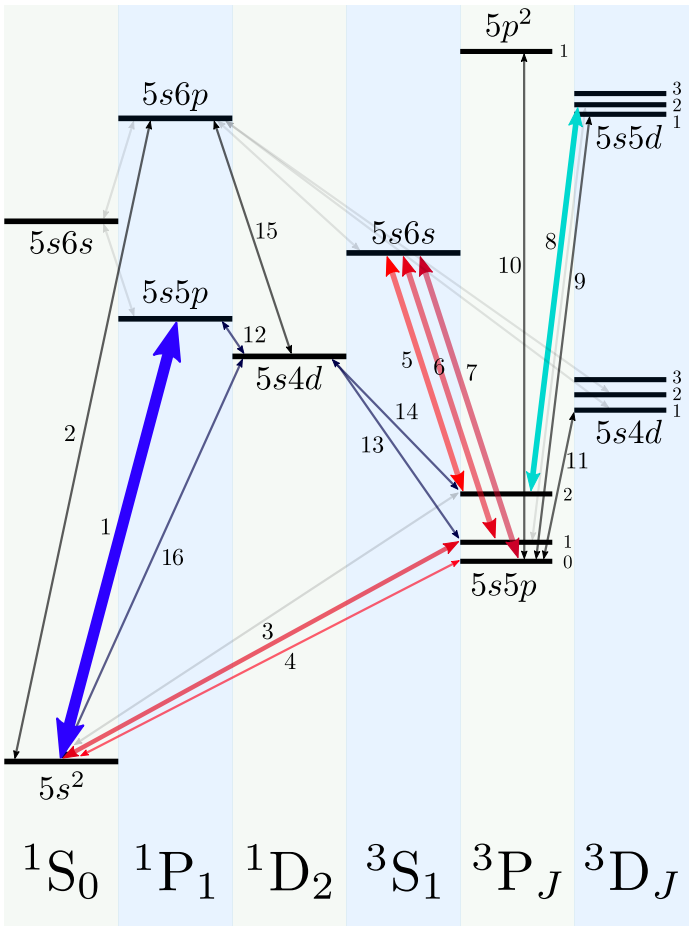
\includegraphics[width=0.4\linewidth]{Figures/Sr.png}
    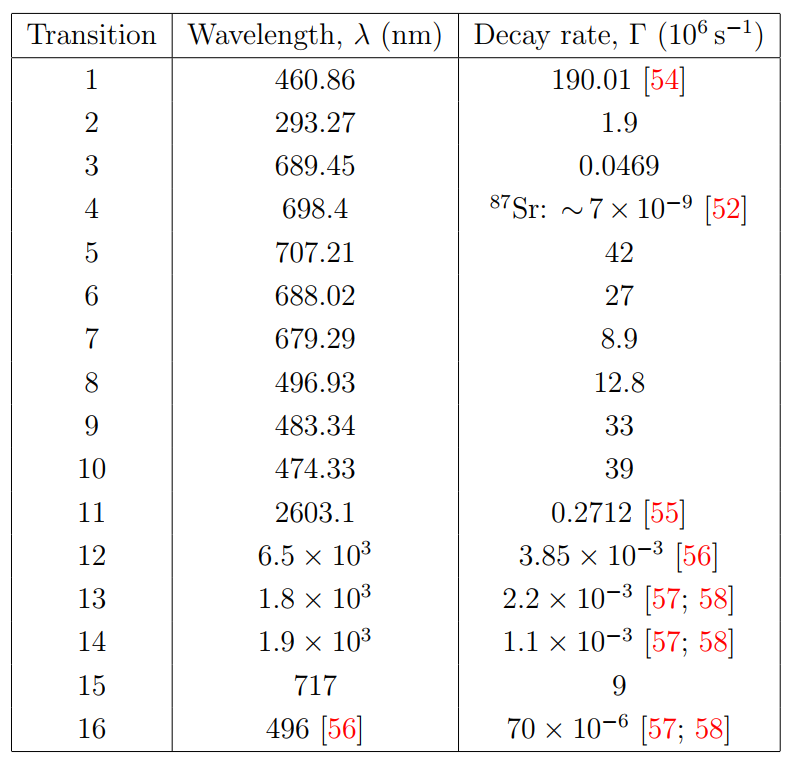
\includegraphics[width=0.4\linewidth]{Figures/Sr2.png}
    \caption{Laser system For $^{88}Sr$ experiments (Referred from lab notes)}
    \label{fig:laser}
\end{figure}
The transition corresponding to 461nm is associated with the Line $1$. This transition exhibits a broad linewidth, enabling rapid and efficient Zeeman cooling and the implementation of a first-order Magneto-Optical Trap (MOT). The 461nm wavelength corresponds to the spectral line of the transition from the ground state to the excited state, making it suitable for precision frequency control using atomic spectroscopy techniques. A commonly employed apparatus for confining neutral atoms involves the integration of optical and magnetic fields, known as a Magneto-Optical Trap (MOT).
\paragraph*{Laser frequency locking---\!\!\!}
In cold atomic experiments, where the laser must interact with the atomic hyperfine energy levels, stringent requirements are imposed on the stability and precision of the laser frequency. Typically, an active frequency stabilization method, referred to as "locking," is employed in this context to ensure the stability of the laser's frequency. Frequency locking is based on the principle of negative feedback. Initially, a reference frequency is established, and then, through specific methods, the laser's frequency is compared to this reference frequency. This process generates an error signal, with the magnitude of the error signal indicating the extent to which the laser frequency deviates from the reference frequency. Employing a designated algorithm, the laser's frequency is then feedback-controlled based on this error signal, reducing the deviation from the reference frequency.
\begin{figure}
    \centering
    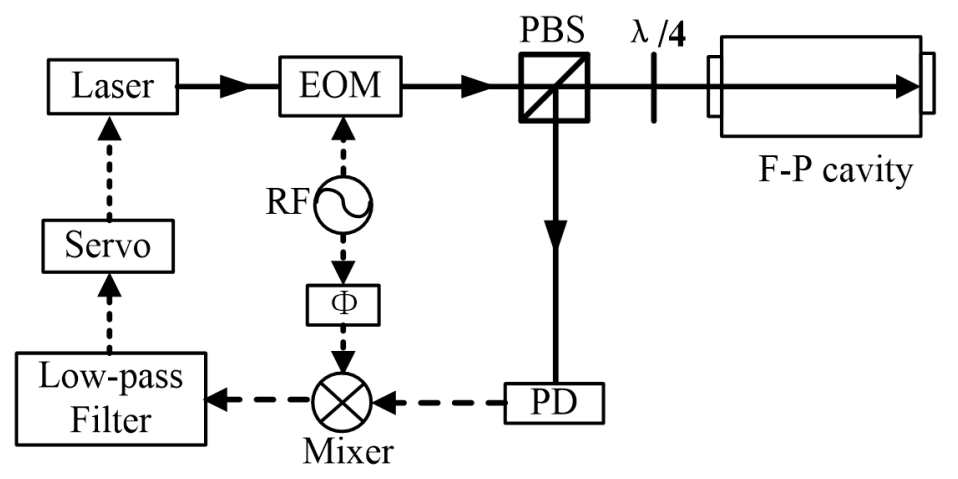
\includegraphics[width=0.5\linewidth]{Figures/PDH lock.png}
    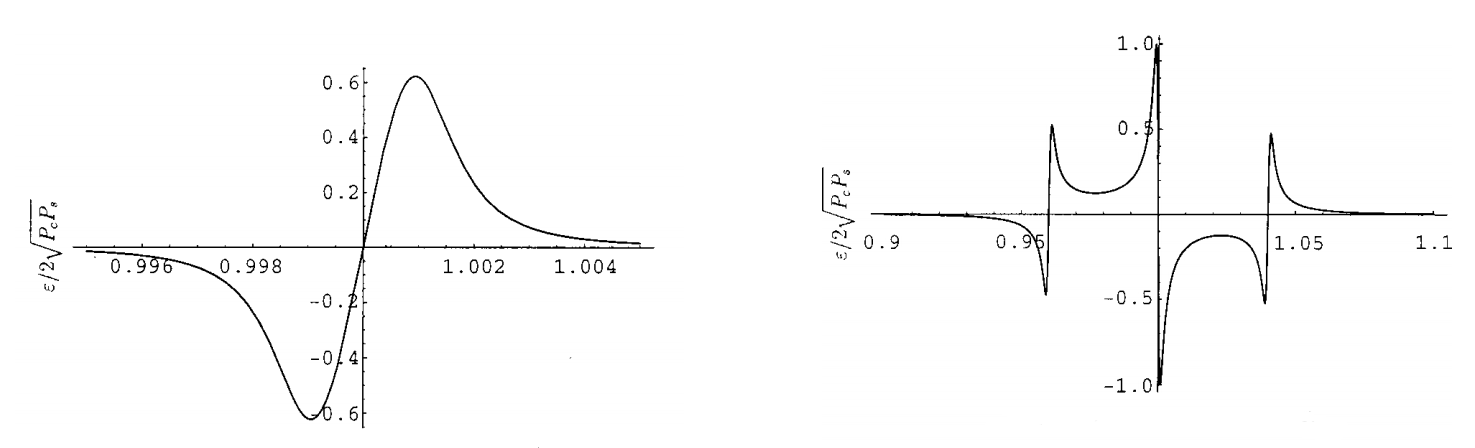
\includegraphics[width=1.0\linewidth]{Figures/PDH error.png}
    \caption{The devices used in frequency locking.}
    \label{fig:PDH_lock}
\end{figure}
Here we mainly introduce the procedure of PDH-locking, which realized laser with  wave-width under $Hz$ magnitude thus will be useful for the clock state transitions. The process is showed in Fig~\ref{fig:PDH_lock}. The laser with $\omega_0$ first pass the\textbf{ electro-optic modulator(EOM)}. This devices is drive by a electronic signal $\beta \sin(\Omega t)$ and will modulate the laser into
\begin{align}
    E_1 &= E_0 e^{i\omega_0 t + i \beta \sin(\Omega t)} \\
    &\approx E_0 e^{i\omega_0 t} + \frac{1}{2} J_1(\beta) E_0 e^{i(\omega_0 + \Omega) t} - \frac{1}{2} J_1(\beta) E_0 e^{i(\omega_0 - \Omega) t} ,
\end{align}
where $J_{\alpha}$ is the Bessel functions and we ignore all the $\alpha > 1$ terms because $\beta$ is small. Then this modulated laser propagate into the \textbf{Fabry-Pérot cavity(F-P cavity)}, which coupling and reflect the laser. It could be proved that the reflection rate of a coupling light with frequency $\omega$ is
\begin{align}
    F(\omega) = r \frac{1 - e^{-i\omega 2L /c}}{1 - r^2 e^{-i\omega 2L/c}}.
\end{align}
For $\omega_n = n \times 2\pi c /2L  $ , $F(\omega_n) = 0$, which means no reflect light should be detected. To realized the coupling, the waist-radius plane of the input Gaussian beam should coincide with the input flat mirrors and so did the beam first reflected by the concave mirror. Further beam pattern matching is also required through charge-coupled device(CCD). \textbf{Photometric detector(PD)} is then used to detect the intensity of the reflected light and output a proportional signal. Considering the mudulation of EOM, the intensity should be
\begin{align}
    I_R &= E_0^2 |F(\omega_0)|^2 + \frac{1}{4} J_1(\beta)^2 E_0^2 |F(\omega_0 + \Omega)|^2 + \frac{1}{4} J_1(\beta)^2 E_0^2 |F(\omega_0 - \Omega)|^2 \notag \\
    &+J_1(\beta) E_0^2 Re[F(\omega_0)F^*(\omega_0 + \Omega) - F^*(\omega_0)F(\omega_0 - \Omega)  ] \cos(\Omega t) \notag \\
    &+J_1(\beta) E_0^2 Im[F(\omega_0)F^*(\omega_0 + \Omega) - F^*(\omega_0)F(\omega_0 - \Omega)  ] \sin(\Omega t).
\end{align}
Then the PD will output a signal to the Signal Mixer with a delayed driving signal $\beta \sin(\Omega t + \Phi)$. The Mixer product this two signal and the followed Low-Pass filter only keeps the magnetitude of oscillating terms $\cos(\Omega),\sin(\Omega)$ in the signal, which is related to $F(\omega_0)F^*(\omega_0 + \Omega) - F^*(\omega_0)F(\omega_0 - \Omega)$. We plot the shape of this function with respect to $\omega_0$ in  Fig~\ref{fig:PDH_lock}, where originals corresponds to $\omega_0 = \omega_n$. This function is monotonic at original, which then serves to the feedback-controlled circuits.

\subsection{Trapping and cooling methods}
Laser cooling of $^{88}Sr$ atoms into a magneto-optical trap (MOT) have been realized long times ago~\cite{PhysRevA.70.063413}. 
The atomic beam is generated from an effusion oven in $525 ^\circ C$ and a measured flux of $3 \times 10^{11}$ atoms per second. 
This atomic beam is then transversely cooled by a two dimensional linearly polarized $461nm$ \textbf{optical molasses.}
To explain this theoretically, we first consider two orthogonal linearly polarized laser plane waves propagates along opposite directions of $z$ axis. 
We know that:
\begin{align}
    \mathbf{E}(z,t) &= \mathcal{E}^+(z) e^{-i\omega t} + c.c., \\
\text{where,~} \mathcal{E}^{+}(z) &= \mathcal{E}_0 \epsilon_x e^{ikz} + \mathcal{E}_0 \epsilon_y e^{-ikz} \\
&=\mathcal{E}_0 \sqrt{2} \left( \cos kz \frac{\epsilon_x + \epsilon_y}{\sqrt{2}} - i \sin kz \frac{\epsilon_y - \epsilon_x}{\sqrt{2}}\right)
\end{align}
We can then see that the polarization is linear along $(\epsilon_x + \epsilon_y)/\sqrt{2}$ at $z = 0$, circular (Left) at $z = \lambda / 8$, linear along $(\epsilon_x - \epsilon_y)/\sqrt{2}$ at $z = \lambda / 4$, and again circular (Right) at $z = 3\lambda / 8$. 
\begin{figure}[!htbp]
\begin{minipage}[t]{0.4\textwidth}
    \centering
    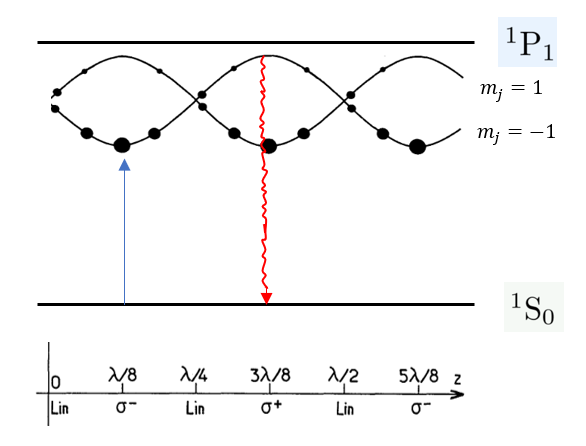
\includegraphics[width=1\linewidth]{Figures/optical molasses.png}
    \caption{Enter Caption}
    \label{fig:optic-molasses}
\end{minipage}
\hspace{0.1\textwidth}
\begin{minipage}[t]{0.4\textwidth}
\centering
    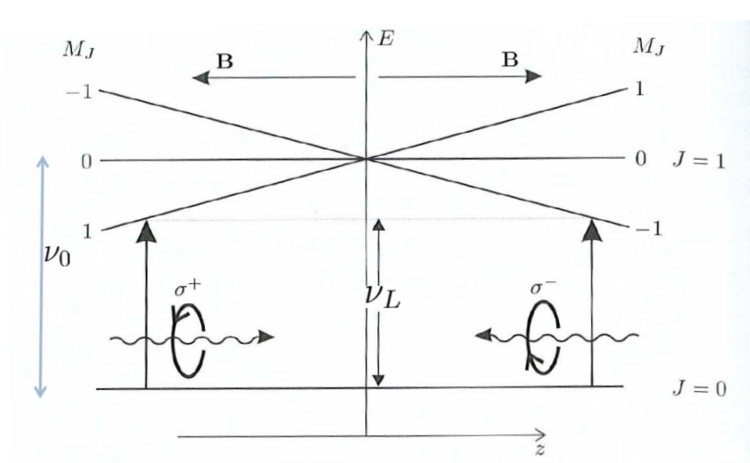
\includegraphics[width=1\linewidth]{Figures/MOT.png}
    \caption{Enter Caption}
    \label{fig:MOT}
\end{minipage}
\end{figure}
This periodic polarization structure along $z$-axis, as depicted in Figure~\ref{fig:optic-molasses}, then generate a spacial periodic Rabi frequency and periodic AC-stark shift for atoms .
Based on all these effects, atoms intend to be stimulated on lower shifted energy level (Black circle with huge size).
The non-zero velocity then leads atoms to climb to the point where polarization shifted and then decay to $^1S_0$ again. 
Such a cooling scheme is sufficient to cold the atoms temperature below the Doppler limit.
After this transverse cooling region, the atomic beam enter a \textbf{Zeeman slower}, which use linearly increased magnetic field to compensate the Doppler detuning. 
Then the atoms move into the trapping chamber, which is evacuated by ion pump and titanium sublimation pump. 
Noted that trapping chamber and oven chamber is connected through a differential pumping tube.
In the trapping chamber, 3-dimensional circularly-polarized $461nm$ cooling and trapping light with detuning $-40MHz$, $1/e^2$ diameters of  $3cm$ and total power $30 mW$ are produced. 
An axial magetic field gradient lies along the gravity direction is generated by a anti-Helmholtz coils.
Current in the coils is regulated by a computer controlled servo and monitored with a Hall probe in order to control the coil center and linearity. 

The combination of this magnetic field gradient and lasers constitute the \textbf{magnetic optical trap (MOT)} of atoms, as shown in Figure~\ref{fig:MOT}. 
Atoms first cooled by Doppler cooling effect. 
Additionally, any atoms diverge from the zero point of magnetic field will induced a Zeeman shift and thus resonance and absorb lasers with opposite momentum.  
As shown in Figure~\ref{fig:sisyphus}, operation of $^1S_0 - {^1P_1}$ MOT will populate $^3P_2, ^3P_1$ state through radiative decay.
When atoms accumulate in those states, the $^1S_0 - {^1P_1}$ MOT scattering force decrease and atoms loss from the trap
Consequently, we use $707nm~^3P_2 - {^3S_1}$ transition and $679nm~^3P_0-{^3S_1}$ transition to repump them back to $^3P_1$ state through decay from $^3S_1$ state to $^3 P_1$. 
Those repump lasers extend the Blue-MOT lifetime from $50ms$ to $500ms$ with the existence of $689~^1S_0 - ^3P_1$ red MOT laser.

\subsubsection{Sisyphus cooling criteria}

The scheme of Sisyphus cooling is showed in the  Figure~\ref{fig:sisyphus}~\cite{Covey_2019}. 
The excited state $^3P_1$ experiences a stronger light shift and tweezers trapping potential compared to the ground state $^1S_0$. 
Such a condition could be satisfied through using linearly polarized trapping light in wavelength ranging from $(700nm,900nm)$~\cite{Covey_2019}.  
In addition to this, the $689nm$ transition has narrow line-width compared to the difference of trapping potential.
This indicates that appropriate red detuning from $689nm$ can selectively excited the atoms near the bottom of the potential.
Due to the long lifetime of $^3P_1$ state, atoms near the bottom then has sufficient time to climbing the sharper potential trap of $^3P_1$  before decay to $^1S_0$ again. 
The temperature of the atoms then will decrease during this process.


\subsubsection{Side-band cooling in atoms arrays}



\subsection{Optical tweezers array}
\subsubsection{Optical tweezers}
The amplitude distribution on the front and rear focal planes of an ideal lens differs by a Fourier transform. For a slight deviation from the position of the rear focal plane, the amplitude distribution can be approximated. Considering the amplitude distribution $\epsilon_i(x',y')$ on the front focal plane, the amplitude distribution on a plane at a slightly shifted position to the right of the rear focal plane at position z can be readily obtained as:
\begin{align}
    \epsilon(x,y,z) = e^{ikz} \frac{k}{2\pi f} \int dx' dy' \epsilon_i(x',y') e^{-ik\frac{xx'+yy'}{f}}
 e^{-ikz\frac{x'^2+y'^2}{2f^2}}.
 \end{align}
 When the incident light is a Gaussian beam with a waist of $w_i$, the amplitude distribution of the light at the right focus of the lens is given by:
 \begin{align}
     \epsilon(r,z) = e^{ikz} \frac{k \epsilon_i}{f} \int_0^R dr' r' e^{-\frac{r'^2}{w_i^2} } J_0(\frac{k}{f} rr') e^{-ikz \frac{r'^2}{2f^2}}.
 \end{align}
Here, $R$ represents the aperture size of the lens. The optical trapping employs far-red-detuned light, causing the primary influence on atoms to be the dipole force, and they tend to concentrate in regions of maximum light intensity (where the equivalent potential energy is minimized), particularly around the focal point. Therefore, the intensity of light near the focus determines the depth of the optical trapping, and the stronger the light intensity, the deeper the potential well. The variation of $|\epsilon(0,0)|^2$ with the parameter $w_i/R$ is depicted in Figure~\ref{fig:twzdepth} as reported in~\cite{ThesisMIT}.
 \begin{figure}
 \begin{minipage}[t]{0.4\textwidth}
         \centering
    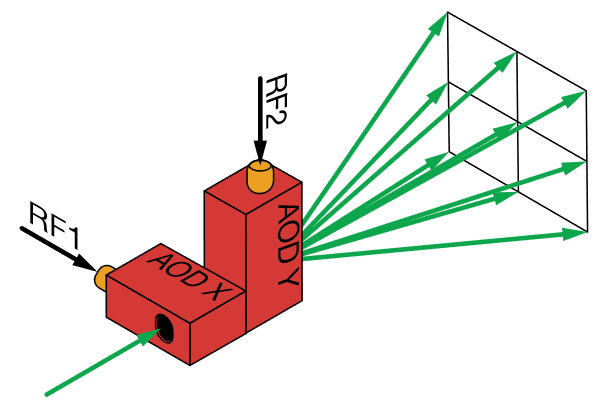
\includegraphics[width=1\linewidth]{Figures/aodprin.png}
    \caption{AOD devices induced atoms array.}
    \label{fig:aodprin}
 \end{minipage}
 \hspace{0.1\textwidth}
 \begin{minipage}[t]{0.4\textwidth}
     \centering
     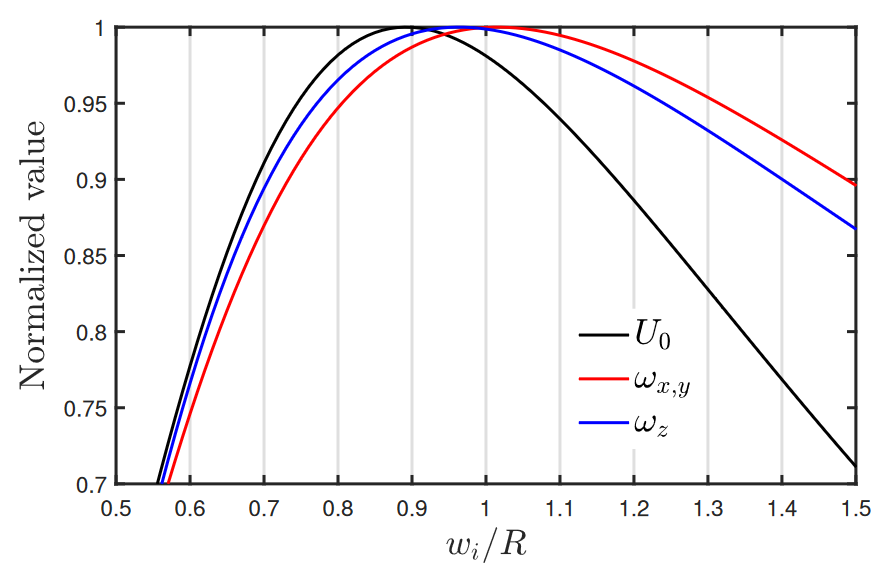
\includegraphics[width=1\linewidth]{Figures/twzdepth.png}
     \caption{ The variation of $|\epsilon(0,0)|^2$ with the parameter $w_i/R$. }
     \label{fig:twzdepth}
 \end{minipage}
     
 \end{figure}
 From the graph, it is evident that when the waist size of the beam and the aperture size of the lens are approximately equal, the trapping depth is maximized. The motion near the center of the potential well can be approximated as harmonic, with a characteristic frequency $\omega$ related to the waist size. Notably, the vibrational frequencies in the xy-plane and the z-plane differ. Subsequently, this frequency can be utilized for sideband cooling of individual atoms in the optical trap. As depicted in the graph, when the waist size of the beam and the aperture size of the lens are nearly equal, the vibrational frequency is maximized, implying a larger splitting of vibrational energy levels. This suggests the potential to cool individual atoms to lower temperatures. In experimental setups, it is common to align the waist size of the Gaussian beam closely with the aperture size of the lens for optimal results.

\subsubsection{Trapping and polarization}
The introduction of tweezers laser in atom system actually add an interaction Hamiltonian as:
\begin{align}
    H_{\text{eff}} &= - \frac{I}{2c\varepsilon_0}\left(\alpha_s + \frac{i\alpha_v}{J}(\hat{\varepsilon}^* \times \hat{\varepsilon})\cdot \vec{J} + \frac{\alpha_t}{2J(2J - 1)}(3\{\hat{\varepsilon}\cdot \vec{J},\hat{\varepsilon}^*\cdot \vec{J}\}) - 2J(J+1)\right) \\
    &:=- \frac{I}{2c\varepsilon_0} \alpha(\vec{J},\hat{\varepsilon})
\end{align}
This effective operator changed with intensity, induced energy shifts and mixing of states with distinct $m_J$. The eigenvalue of operator $\alpha$ under given quantum number $J$ gives $2J+1$ energy shifts with respect to the original degenerate energy level of state $\ket{J,m_J}$. For positive eigenvalues, atoms tends to bounded in the focal point of tweezers while for negative eigenvalues atoms will be expelled out of the tweezers. Thus ones have to choose an appropriate wave-length and polarization for the tweezers. In previous research by Madjarov \emph{et.al.}~\cite{ThesisMIT}, they choose $\lambda = 813.4\text{nm}$, which induced identical shifts for state $\ket{5s5s~^{1}S_0}$ and    $\ket{5s5p~^{3}P_0}$.
 \subsubsection{Tweezers Arrays}
To create an array of neutral atoms, it is essential to confine the atoms in a series of optical traps with equal optical frequencies, trapping depths, trapping vibrational frequencies, and spacing between the traps. Achieving such a uniformly structured multi-focus optical trapping field is often realized using spatial light modulators (SLMs) or acousto-optic deflectors (AODs).
\paragraph{Atoms array based on AODs}
Acousto-optic deflectors (AODs) guide laser beams through a medium, causing the medium to oscillate under the influence of an electrical signal, leading to periodic changes in the refractive index in space. The periodic modulation of refractive index scatters the laser's phase, allowing it to transform into multiple laser beams propagating in different directions. This process can be conceptualized as the scattering of photons by phonons. Scattering occurs when satisfying the Bragg condition, wherein the photon momentum $\Vec{k_o}$ and phonon momentum $\Vec{k_a}$ must meet the following criteria:
\begin{align}
    \Vec{k_o} \cdot \Vec{k_a} = \frac{1}{2}(\frac{c_s^2 - c^2}{cc_s})\frac{\omega_s}{\omega_i} + \frac{c_s}{c}
\end{align}
In most AOD devices, the Bragg condition is configured such that the photon and phonon momenta are perpendicular, allowing for the lateral alteration of the photon's momentum direction:
\begin{align}
    \Delta \theta = \frac{c}{c_s} \frac{n\omega_a}{\omega_o}, n = 0,\pm 1,\pm 2,\cdots
\end{align}

As illustrated in Figure~\ref{fig:aodprin}, when the exit plane of the AOD is positioned at the left focus of the lens, multiple bright spots will appear at the right focus of the lens, resembling the scenario of a single Gaussian beam incident. This results in the creation of a uniform optical trapping array.

One drawback of this approach is the slight variation in the optical frequencies of different traps, leading to disparate shifts in clock states. Additionally, when traps are closely spaced, the frequency mismatch causes heating effects at the edges of the traps, impacting the efficiency of subsequent sideband cooling.
\paragraph{Atoms array based on SLMs}
The Fourier transform on the double focal planes of the lens is given by:
\begin{align}
    \epsilon(x,y) =  \frac{k}{2\pi f} \int_{-\infty}^{\infty} dx' dy' \epsilon'(x',y') e^{-2\pi i \frac{xx'+yy'}{\lambda f}}.
 \end{align}
 Given that the liquid crystal plane of the SLMs is finite, and functions on it can only be sampled at discrete pixel points rather than continuous functions, the algorithm sets the sampling intervals on the left focal plane to be the pixel size $\Delta$. The number of samples in the $x'$ and $y'$ directions is denoted by $N_x'$ and $N_y'$. The finite and discrete phase distribution $\epsilon(x',y')$ on the liquid crystal screen is periodically extended to the entire plane of the left focal point. The phase distribution function on the liquid crystal screen is approximated as the sum of delta functions at several sampling points. The integral mentioned above can be expressed as:
  \begin{align}
    \epsilon(x,y) &=  A\sum_{q=0,\pm 1,\cdots}  e^{-2\pi i \frac{q(L_x' x+L_y' y)}{\lambda f}} \int dx' dy' \sum_{m',n'}  \epsilon'(x',y')\delta(x' - x'_{m'})\delta(y' - y'_{n'}) e^{-2\pi i \frac{xx'+yy'}{\lambda f}} \notag \\
    &= A\sum_{q=0,\pm 1,\cdots} e^{-2\pi i \frac{q(L_x' x+L_y' y)}{\lambda f}}  \sum_{m',n'} \epsilon_{m',n'} e^{-2\pi i \frac{x m' \Delta +y n' \Delta }{\lambda f}}.
 \end{align}
Here, $L_x' = N_x' \Delta$, $L_y' = N_y' \Delta$, and $m'= 0,\cdots, N_x'-1, n'= 0, \cdots, N_y' -1$. For points on the right focal plane, $\frac{L_x' x}{\lambda f} = 0, \pm 1, \cdots$. The first part of the summation only contributes to coherent reinforcement, resulting in the strongest intensity. Therefore, the periodic extension on the left focal plane is equivalent to retaining only these points of coherent reinforcement on the right focal plane, representing the approximate centers of the optical tweezers array. The positions and amplitudes of the optical tweezers are then given by:
 \begin{align}
     (m,n) \to& (x_m,y_n) = (\frac{\lambda f m}{N_x \Delta}, \frac{\lambda f n}{N_y \Delta}), \\
     \epsilon_{m,n} &= A \sum_{m' = 0}^{N_x -1}\sum_{n' = 0}^{N_y -1} \epsilon_{m',n'} e^{-2\pi i (\frac{m m' }{N_x'} +\frac{n n' }{N_y'})}.
 \end{align}
 The amplitude distribution of each optical tweezer on the right focal plane is evidently the discrete Fourier transform of the amplitude distribution of sampling points on the left focal plane. While $m$ and $n$ can take any values, the distribution $\epsilon_{m,n}$ also exhibits periodicity with $N_x$ and $N_y$. Therefore, it is generally preferable to choose $m \in \left(-\frac{N_x}{2}, \frac{N_x}{2}\right)$ and $n \in \left(-\frac{N_y}{2}, \frac{N_y}{2}\right)$ to ensure the accurate representation of the intensity distribution around the lens center. However, common computational software often simplifies calculations by taking $m = 0,\cdots, N_x - 1$ and $n = 0,\cdots, N_y - 1$, corresponding to points on the screen in the range of $x, y \in \left[0, \frac{\lambda f}{\Delta}\right)$. To align it correctly with the center, a translation is typically applied. Additionally, in experimental setups, a simple inverse Fourier transform of the amplitude on the right focal plane does not yield the correct optical tweezer field due to approximations introduced by periodicity and sampling points. To address this, the Weighted Gerchberg-Saxton (WGS) algorithm is commonly employed.
\begin{figure}
    \centering
    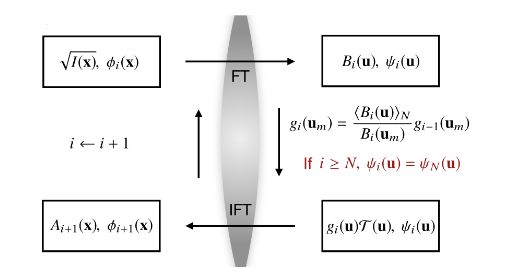
\includegraphics[width=0.5\linewidth]{Figures/WGSal.png}
    \caption{Weighted Gerchberg-Saxton (WGS) algorithm to generate uniform tweezers array}
    \label{fig:WGS}
\end{figure}

\begin{algorithm} 
	\caption{WGS Algorithm} 
	\label{alg:WGS} 
	\begin{algorithmic}
		\REQUIRE  
  the Fourier transformation sampling numbers, denoted as $N_x$ and $N_y$. \\
  Initial distribution $L_0$ on the left focal plane, derived based on the specified sampling numbers.\\
  The desired intensity distribution $E$ on the right focal plane.\\
  A predetermined number of iterations $N$ and an unchanged phase threshold $t$. \\
  It is crucial to highlight that all subsequent matrix multiplications are performed pointwise.
		\ENSURE $L_N$ approximates the generation of the desired intensity distribution $E$.
        \STATE $i = 0, g = 1$.
        \STATE $E_{\text{mask}} \gets \mathbf{MASK}(E)$, where $\mathbf{MASK}$ transforms non-zero elements of the input matrix to 1, leaving zeros unchanged.
        \WHILE{$i < N$}
		\STATE $R_i \gets \mathbf{fft}(L_i)$ 
        \STATE $R_{mask_i} \gets E_{mask} \times R_i$ 
        \STATE $g_i \gets g \times \frac{|R_{\text{mask}_i}|}{\bar{R}{\text{mask}_i}}$, where $\bar{R}_{\text{mask}_i}$ represents the average value of all non-zero elements in the matrix.
        \IF{$(\max{|R_{mask_i}|/\bar{R}_{mask_i}} - 1 > t$ \&\& $i > 0)$}
        \STATE $phase_i \gets phase(R_{mask_i})$
        \ELSE
        \STATE $phase_i \gets phase_{i - 1}$
        \ENDIF 
        \STATE $R_i' \gets E\times g_i \times phase_i$
        \STATE  $L_{i+1}' \gets \mathbf{ifft}(R_i')$ 
        \STATE  $L_{i+1} \gets |L_0|\times phase(L_{i+1}')$ 
        \STATE $i \gets i+1$
        \ENDWHILE 
	\end{algorithmic} 
\end{algorithm}

 As illustrated in Figure~\ref{fig:WGS} and outlined in Algorithm~\ref{alg:WGS}, the Weighted-Gerchberg Saxton (WGS) algorithm begins with a randomly phased Gaussian light as the initial input. It iteratively performs Fourier transforms on both the left and right focal planes while continuously updating the right focal plane's intensity with the desired intensity and replacing the left focal plane's intensity with the input Gaussian light's intensity. Additionally, when the light distribution in the right focal plane becomes sufficiently uniform, the phase iteration on the right focal plane remains unchanged. This iterative process yields a high-precision phase distribution $phase(L_N)$ that the Spatial Light Modulator (SLM) should generate. The sampling points for the Fourier transform, denoted as $N_x$ and $N_y$, may exceed the resolution of the SLM. In such cases, the central maximum square of sampling points is considered for the SLM's phase distribution.
 \subsubsection{Rearrangement of arrays}
 

\subsection{Single atom imaging\label{subsec:single_atom_image}}
Imaging step try to determine the presence or absence of an atom while not expel the atom from the trap. 
Most experiments stimulate ground state atom($^1S_0$) into $^1P_1$ state with 461nm lasers and use an electron-multiplying charge-coupled device camera  (EMCCD)  to observed the fluorescence light. 
In the meantime, to avoid the heating effect of the light recoil, we cool the atom using $^1S_0 - ^3P_1$ transition at 689nm and Sisyphus scheme. 

The scattering of fluorescence photons is described by dipole radiation pattern $\mathcal{D}(\theta,\phi)$ that giving the probability that an atom will scatter a photon in a particular direction. In the imaging process, we consider the transition $\ket{J = 0, m_J = 0 }$ to $\ket{J =1 , m_J = 0,\pm 1 }$ only and write:
\begin{align}
    \mathcal{D}(\theta,\phi) &= \frac{3}{8\pi} \sin^2(\theta)~[\text{to}~m_J = 0],\\
    \mathcal{D}(\theta,\phi) &= \frac{3}{16\pi} (1 + \cos^2(\theta))~[\text{to}~m_J = \pm 1],
\end{align}
,where $\theta$ is the angle between quantization axis. Proof could be found on textbook~\cite{steck_optic_atoms}. This give the optimal direction to observe the fluorescence photons for different transitions.
\subsection{Single atom production}
The pairwise loss method allows atoms within the optical tweezers to escape in pairs. In this process, specific-frequency lasers are directed onto neutral atoms within the optical tweezers. Under laser excitation, two atoms combine to form an excited state diatomic molecule, subsequently spontaneously radiating from the excited state to the ground state. The resulting kinetic energy is sufficient to enable the escape of the diatomic molecule from the optical tweezers.

\begin{enumerate}
    \item Transport atoms from the red MOT (Magneto-Optical Trap) into the optical tweezers.
    \item Introduce lasers to implement pairwise loss.
    \item Observe the presence of atoms in each optical tweezer, recording the tweezers containing atoms.
    \item Excite all atoms to the clock state.
    \item Adjust AOD (Acousto-Optic Deflector) signals to reduce the depth of tweezers containing atoms.
    \item Reload atoms from the red MOT into the tweezers. Tweezers that initially had a single atom now contain one atom in the clock state and several in the ground state, while tweezers without atoms consist entirely of ground-state atoms.
    \item Introduce imaging and cooling light to all tweezers simultaneously. These lights have no impact on clock-state atoms but cause ground-state atoms in tweezers with shallower depths to overflow, while ground-state atoms in tweezers with deeper depths remain confined.
    \item Adjust AOD signals to restore the original depth of all tweezers.
    \item Return to step 2.
\end{enumerate}



\section{High Fidelity control of Rydberg atoms\label{sec:error_atoms}}
\subsection{Measurements Protocol}

\subsubsection{Destructive measurement protocol}
The fast, non-destructive and high-fidelity measurement methods in neural atom array are properly reviewed previous research~\cite{Shea_measurement}.  In $^{87}Rb$, to mitigate the decoherence effect caused by magnetic field noise, quantum states are encoded on the two hyperfine levels with m=0, as illustrated in the figure.
\begin{figure}[!htbp]
\begin{minipage}[t]{0.4\textwidth}
        \centering
    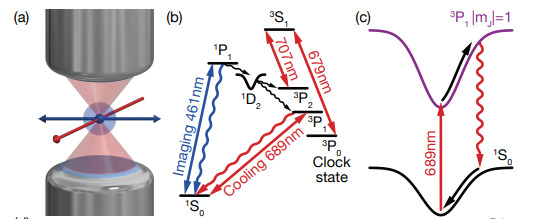
\includegraphics[width=1\linewidth]{Figures/sisyphus.png}
    \caption{The imaging and cooling method and Sisyphus scheme.}
    \label{fig:sisyphus}
\end{minipage}
\hspace{0.1\textwidth}
\begin{minipage}[t]{0.4\textwidth}
    \centering
    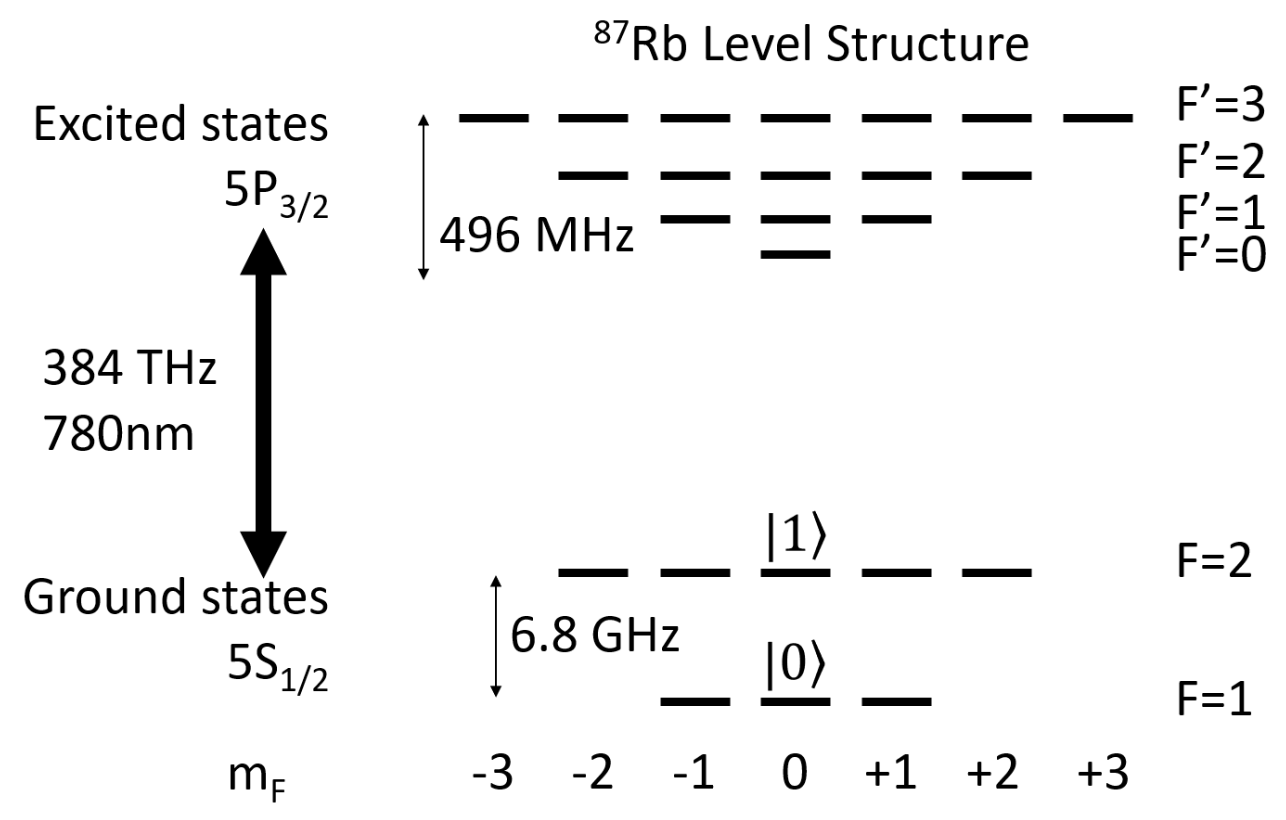
\includegraphics[width=1\linewidth]{Figures/measurementfig.png}
    \caption{The direct measurement scheme in $^{87}Rb$ atoms. }
    \label{fig:enter-label}
    \end{minipage}
\end{figure}
The most direct measurement method utilizes the difference of $780\text{nm}$ laser scattering rates of different hyperfine levels. For the transition from $|1 \rangle,|0 \rangle$ to $5P_{\frac{3}{2}}$, $F' = 3$, the photon scattering rates are on the order of $10^6/s$ and $1/s$ respectively. Hence, a threshold $n_{th}$ for detecting photons can be set, with photons below this threshold classified as $|0\rangle$ state. 
This protocol, through simple in theory, are not practical in experiments
First, it ignore the fact that the $|1\rangle$ state can also be heated, leading to rapid atom loss in shallow optical traps. Due to unknown atom loss, the photon count is insufficient to distinguish from $|0\rangle$ state. Therefore, we have to introduce some cooling scheme and increase the trap depth correspondingly.
Second, the state excited in the $5P_{3/2}$ states has non-zero probability decay to some dark states or back to computational states, which cause measurement error. 
\paragraph*{Push out measurement---\!\!\!}
In the push-out measurement experiment~\cite{PhysRevLett.123.170503},  the atoms in the $\ket{F = 2} $ state are first heated out of the traps by a resonant laser on the $\ket{F = 2} \to \ket{F' = 3}$ transition. Next, the remaining atoms in the $\ket{F = 1}$ state are detected by illuminating them with cooling lasers and collecting the fluorescence photons that similar to the procedure described in subsection~\ref{subsec:single_atom_image}

In practice, this qubit measurement scheme is corrupted by atom loss processes-since an atom in the $\ket{1}$ state is indistinguishable from no atom at all. Therefore, care must be taken to eliminate sources of atom loss, and to make the traps as robust as possible.

\subsection{Single Gate implementation and state initialization}

\paragraph*{Single qubit gates---\!\!\!}
According to the universal quantum gate set, the realization of single-qubit gates and Control-Z gates could approximate any unitary gate. Due to the absence of hyperfine structure in the strontium ground state, one always uses the ground state~($\ket{g}$) $5s^2 ~{^1}S_0$ and clock state~($\ket{c}$) $5s5p~ {^3}P_0$ as a qubit.  We then build the coherent transition between two levels through Rabi oscillation in Eq.~\eqref{eq:Intraction-single-H_S}. This gives the unitary evolution below:
\begin{align}
    U(\frac{\Omega t}{2}, \delta t) = \begin{pmatrix}
        \cos[\frac{\Omega t}{2}] & -i \sin[\frac{\Omega t}{2}]e^{i \delta t} \\
        -i \sin[\frac{\Omega t}{2}] e^{- i \delta t} & \cos[\frac{\Omega t}{2}]
    \end{pmatrix}
\end{align}
Noted that we use interaction picture, which leads to $\ket{0} = e^{-i \frac{\delta}{2} t} \ket{g},\ket{1} = e^{i\frac{\delta}{2} t} \ket{c} $. The measurement of such basis is equivalence to the measurement of clock state and ground state. We noted that different choices of $(\Omega t/2, \delta t) = (\phi,0),(\phi,-\frac{\pi}{2})$ could generate $R_x(\phi)$ and $R_y(\phi)$, whose composition could generate arbitrary single-qubit gates through the equality below: 
\begin{align*}
    U&=e^{i\alpha}\begin{pmatrix}
    e^{i(-\frac{\beta}{2}-\frac{\delta}{2})}cos(\frac{\gamma}{2})&-e^{i(-\frac{\beta}{2}+\frac{\delta}{2})}sin(\frac{\gamma}{2})\\
    e^{i(\frac{\beta}{2}-\frac{\delta}{2})}sin(\frac{\gamma}{2})&e^{i(\frac{\beta}{2}+\frac{\delta}{2})}cos(\frac{\gamma}{2})\\
\end{pmatrix} \\
&=R_z(-\beta)*R_y(-\gamma)*R_z(-\delta)
\end{align*}
The controlling of parameters $\Omega$ and $\delta$ is quite well developed using AOMs and AODs driven by arbitrary wave generators (AWGs). Single operation with low crosstalk has been realized~\cite{PhysRevLett.119.053202}. 

\paragraph*{Optical pumping for initialization---\!\!\!}
In previous experiment, Levine \emph{et. al.}~\cite{PhysRevLett.123.170503} use optical pumping method to transfer states in the ground state manifold $5S_{1/2}$ into hyper-fine state $\ket{0} = \ket{5S_{1/2},F = 1,m_F = 0}$
\begin{figure}
    \centering
    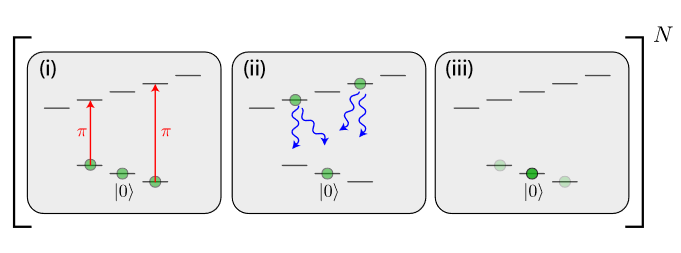
\includegraphics[width=0.5\linewidth]{Figures/initialization.png}
    \caption{The process of optical pumping to prepare qubit at $\ket{0}$ state.~\cite{PhysRevLett.123.170503}}
    \label{fig:initial}
\end{figure}
%%%%%%%%%%%%%%%%%%%%%%%%%%%%%%%%%%%%%%%%%%%%%%%%%%%
\subsection{Multi-qubits gates Protocols}
\subsubsection{Single photon process}
 The Hilbert space of two atoms now constitute with $\ket{0}_i, \ket{1}_i = \ket{g}_i$ and Rydberg state $\ket{r}_i$. The Hamitonian under classical signal $E(t) = \vec{E_0}(t) \cos(\omega_L t + \phi(t))$ is written as:

\begin{align}
    H_{\rm tot} = \sum_{i = 1,2}\hbar (\omega_r - \omega_g)|r\rangle \langle r|_i + \left(\Omega(t)|r\rangle \langle g|_i+c.c.\right)\cos(\omega_Lt + \phi(t)) + B_{12} \ket{rr}\bra{rr}.
\end{align}
Under the time-dependent unitary transformation $U(t) = e^{i(\omega_r - \omega_g)t |r\rangle \langle r|}$, the Hamiltonian now become:
\begin{align}
H'_{\rm tot} &= i\hbar \frac{dU}{dt} U^\dagger + UHU^\dagger \\
&= \sum_{i = 1,2} \left[ \frac{\tilde{\Omega}(t)}{2}|g\rangle \langle r|_i + c.c. \right] +  B_{12} \ket{rr}\bra{rr}.
\end{align}
Now through appropriate choice of the amplitude and phase of $\tilde{\Omega}(t) = e^{i\phi(t) + i[\omega_L - (\omega_r - \omega_g)]t} \times  \bra{r} \vec{E}_0(t) \cdot \vec{\varepsilon} r\ket{g}$, we are able to realized the two-qubits gate between these two atoms.
Similar to the discussion of the Rydberg Blockade effect, state initialized to state $\ket{gg}$ only changes in the subspace spaned by $\ket{gg},  \ket{W} = \sqrt{2^{-1}}(\ket{1r} + \ket{r1})$ and $\ket{rr}$ . The state initialized to state $\ket{0g}$ belong to the subspace $\{\ket{0g},\ket{0r}\}$ and $\ket{00}$ will be a dark states. If $B_{12} \gg \max_{t}|\Omega(t)|$ is further satisfied, the Blockade approximation could be applied. This observation enable the gate protocol being optimized according to two Hamiltonian $H_{q}$ below and vividly expressed through two trajectory on Bloch sphere with two-qubit space spaned by  $\{\ket{0g},\ket{0r}\}$ and  $\{\ket{gg},\ket{W}\}$. 

\begin{align}\label{eq:twoqubit_Ham_withblockade}
    H_{01}&= \frac{\tilde{\Omega}(t)}{2}|01\rangle \langle 0r|_i + c.c. ,\\
    H_{11}&= \frac{\sqrt{2}\tilde{\Omega}(t)}{2}|11\rangle \langle W|_i + c.c. 
\end{align}

\paragraph*{Phase shift protocol---\!\!\!}In the research of Leving et.al. in 2019, a simple laser protocol is first proposed to realize CPHASE gates with $97.4\%$ fidelity~\cite{PhysRevLett.123.170503}. In this protocol,as illustrated in Fig~\ref{fig:phaseshift}, two pulses with the same slight detuning $\Delta$, Rabi frequency $\Omega$, and a phase shift $\xi$ between them drive the transition between state $\ket{g}$ and $\ket{r}$.If one of two qubits is in $\ket{0}$ state, the state changes along the brown line in Fig~\ref{fig:phaseshift}, which moves back into the $\ket{0g}$ state but commulates a phase shift $\phi_{01}$. If both qubits are in the $\ket{1}$ state, due to the Rydberg blockade, states will transfer to $\ket{W} = \sqrt{2^{-1}}(\ket{1r} + \ket{r1})$. State change along the red line, giving a different phase shift $\phi_{11}$. Through changing $\Delta, \Omega$ and $\xi$, ones adjust the phases and implement the control-Z gate.
\begin{figure}[htbp]
\centering
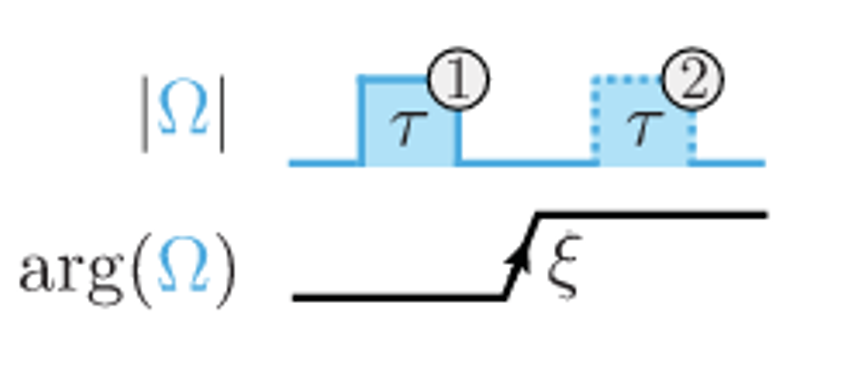
\includegraphics[height=2cm,width=4cm]{Figures/phaseshift_ws.png}
\hspace{0.5in}
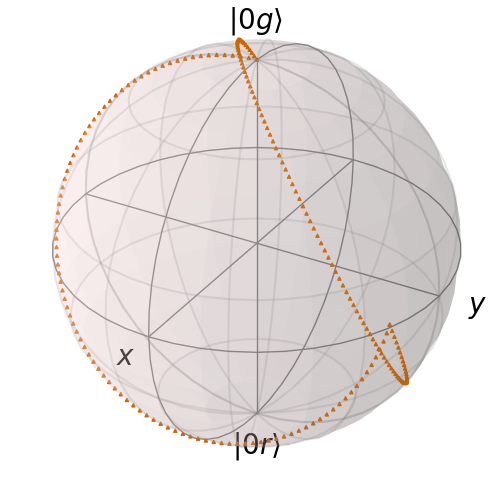
\includegraphics[height=4cm,width=4cm]{Figures/phaseshift_10.png}
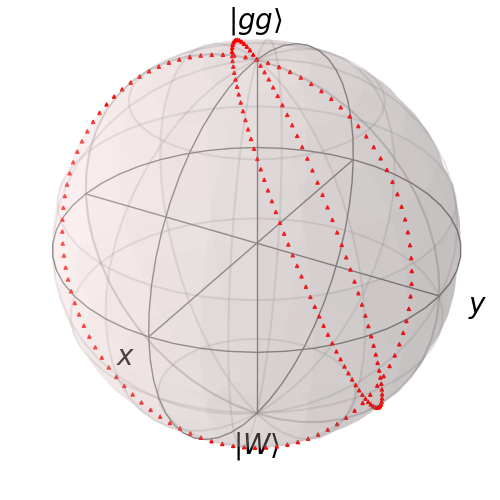
\includegraphics[height=4cm,width=4cm]{Figures/phaseshift_11.png}
\caption{The trace on the Bloch-sphere of the phase-shift protocol for the $\text{CPHASE}$ gate.}
 \label{fig:phaseshift}
\end{figure}
The python code that simulate this protocol is listed in Appendix~\ref{app:gate_codes}.

\paragraph{Time-optimal protocol---\!\!\!}In a recent research, Sven \emph{et al.}~\cite{Jandura_2022} proposed pulses that are optimized using a combination of numerical and semi-analytical quantum optimal control techniques that result in smooth Ansätze with just a few variational parameters. 

In this protocol, laser's Rabi frequency is bounded by $\Omega_{\max}$ and its phase could change as $\phi(t)$. Fastest gate protocol demands $|\tilde \Omega(t)| = \Omega_{\max}$ during the process. To achieve the best gate fidelity under certain fixed gate time $T$ , we use Gradient Ascent Pulse Engineering (GRAPE) to optimized the $\phi(t)$ . 

Inaccurate quantum gates are CPTP maps (completely positive trace preserving maps) from density matrices to density matrices, denoted as $\mathcal{E}$. To measure their similarity to unitary transformations $U(\cdot)U^\dagger$, one method is to quantify the discrepancy between output states under the same input pure state, defining the Average Gate fidelity as follows:
\[
\bar{F}(\mathcal{E},U) := \int d\psi \langle \psi | U^\dagger \mathcal{E}(|\psi \rangle \langle \psi|)U | \psi \rangle
\]
Additionally, utilizing the Choi representation of CPTP maps, one can also define the Entangled Gate fidelity. They are equivalent up to a linear transformation~\cite{Nielsen_2002}. 

In the case of two-qubit \textbf{CPHASE}-gates, the averge gate fidelity could be written as:
\begin{align}
    \bar{F} = \frac{1}{20} (|1 + 2a_{01} + a_{11}|^2 + |a_{11}|^2 + 2|a_{01}|^2 + 1),
\end{align}
where $a_{q} = \langle q|\psi_{q}(T)\rangle$. 
Explicit proof of this equation could be found in Appendix~\ref{app:gate_fidelity}. 

The laser phase function $\phi(t)$ then be divided into $N = 100$ pieces with constant value $c_i$ in each piece.  After this, the explicit value of $a_{01},a_{11}$ could be found through solving time-dependent Schrodinger equation in Eq.~\eqref{eq:twoqubit_Ham_withblockade}.
Then $\bar{F}$ became a function of these parameters. 

\begin{figure}[!hbtp]
    \centering
    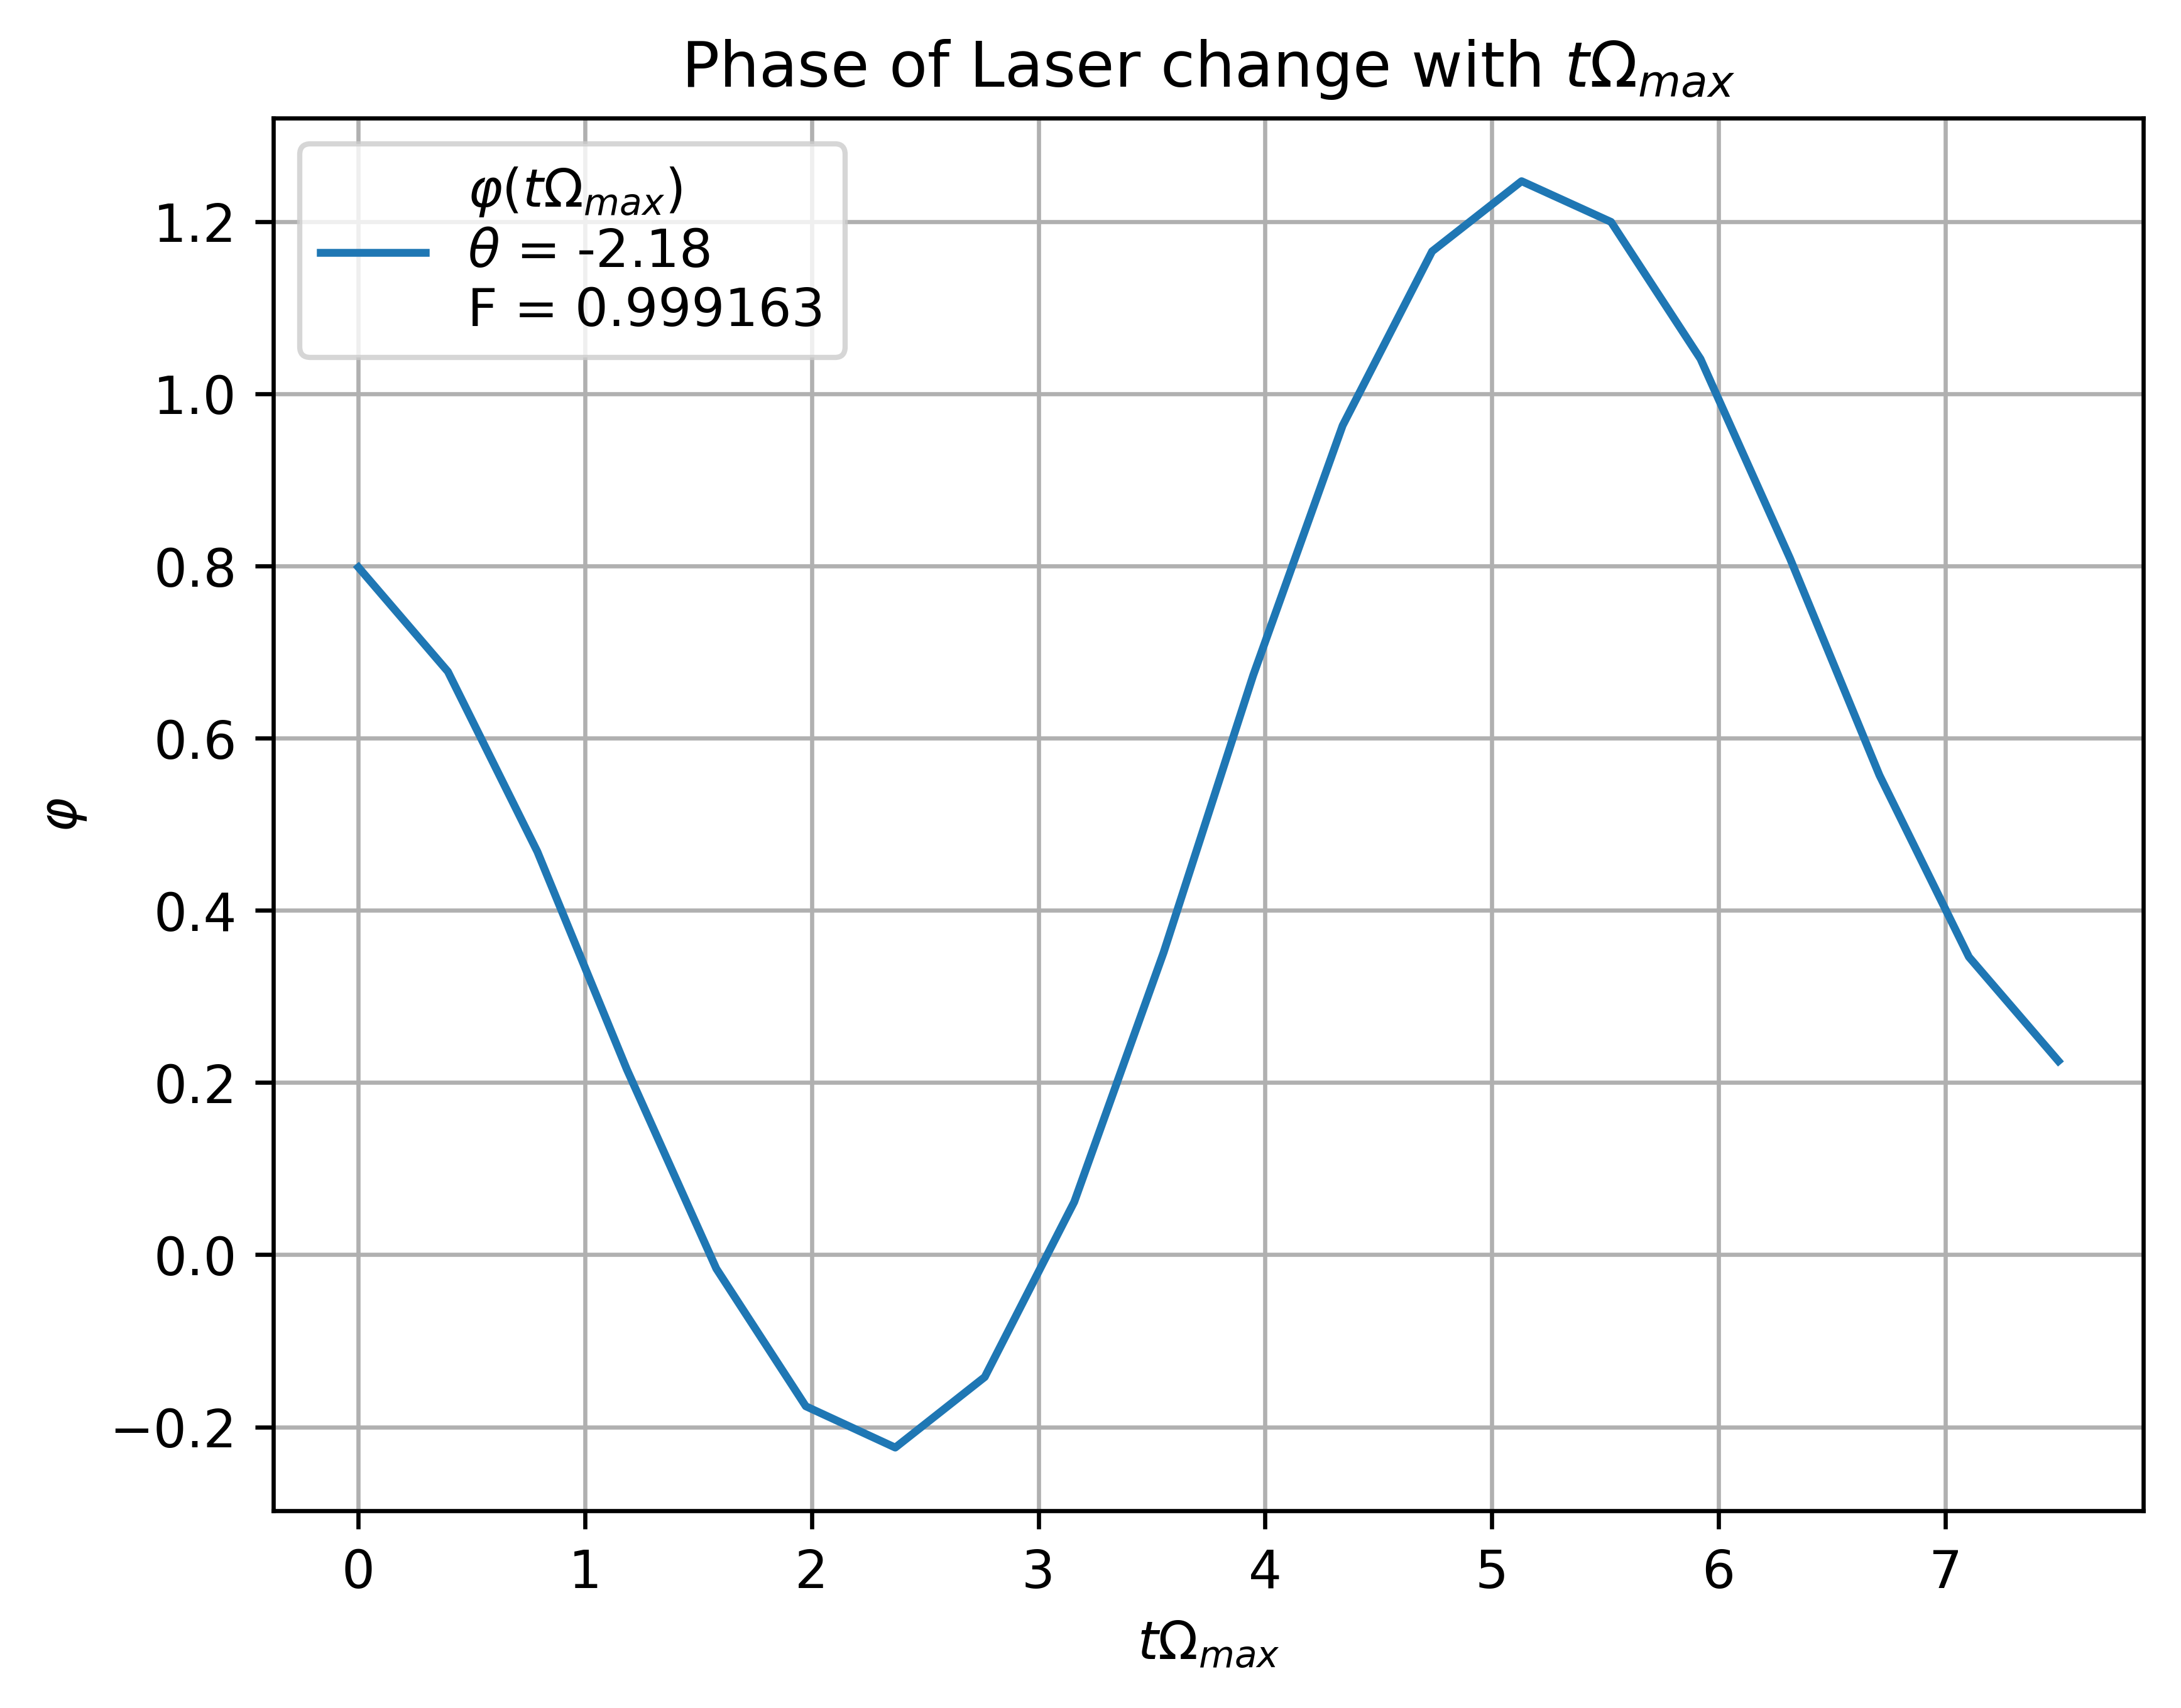
\includegraphics[width=0.5\linewidth]{Figures/time_optimal_idealCZ.png}
    \caption{Time optimal phase wave shape of the laser}
    \label{fig:time_optimal_ws}
\end{figure}
In the codes, we fixed the gate time through  $\Omega_{\max} T = 7.5$  and take $\bar{F}(c_1,\cdots,c_{100})$ as minimized objective function $1 - \bar{F}$.  
Details could be checked on Appendix~\ref{app:gate_codes}.
We also noted that the gate we realized is:
\begin{align}
    \text{CPHASE}(\theta) = 
    \begin{pmatrix}
        1& 0& 0& 0 \\
        0& e^{i\theta}& 0& 0 \\
        0& 0&  e^{i\theta}& 0 \\
        0& 0& 0& e^{2i\theta + i \pi} 
    \end{pmatrix}
\end{align}
This gates could be transformed into the $\text{CZ}$ gate up to a local transformation $\ket{0} \to \ket{0},\quad \ket{1} \to e^{-i\theta} \ket{1}$. Thus $\theta$ is also a possible parameter that could be optimized. 

The optimal wave-shape in Fig~\ref{fig:time_optimal_ws} is similar to the trigonometric function. Thus Evered \emph{et.al.}~\cite{Evered_2023} constructs an smooth Ansätze with fewer variational parameter $\{\delta_0, A,\omega_0,\varphi_0, \theta\}$:
\begin{align}
    \phi(t) = \delta_0 t + A\cos(\omega_0 t - \varphi_0)
\end{align}
This antasaz is almost as fast as the time-optimal protocol above. The trace on the Bloch sphere are ploted on Fig.~\ref{fig:anta-time-optimal}.
\begin{figure}[!hbtp]
\centering
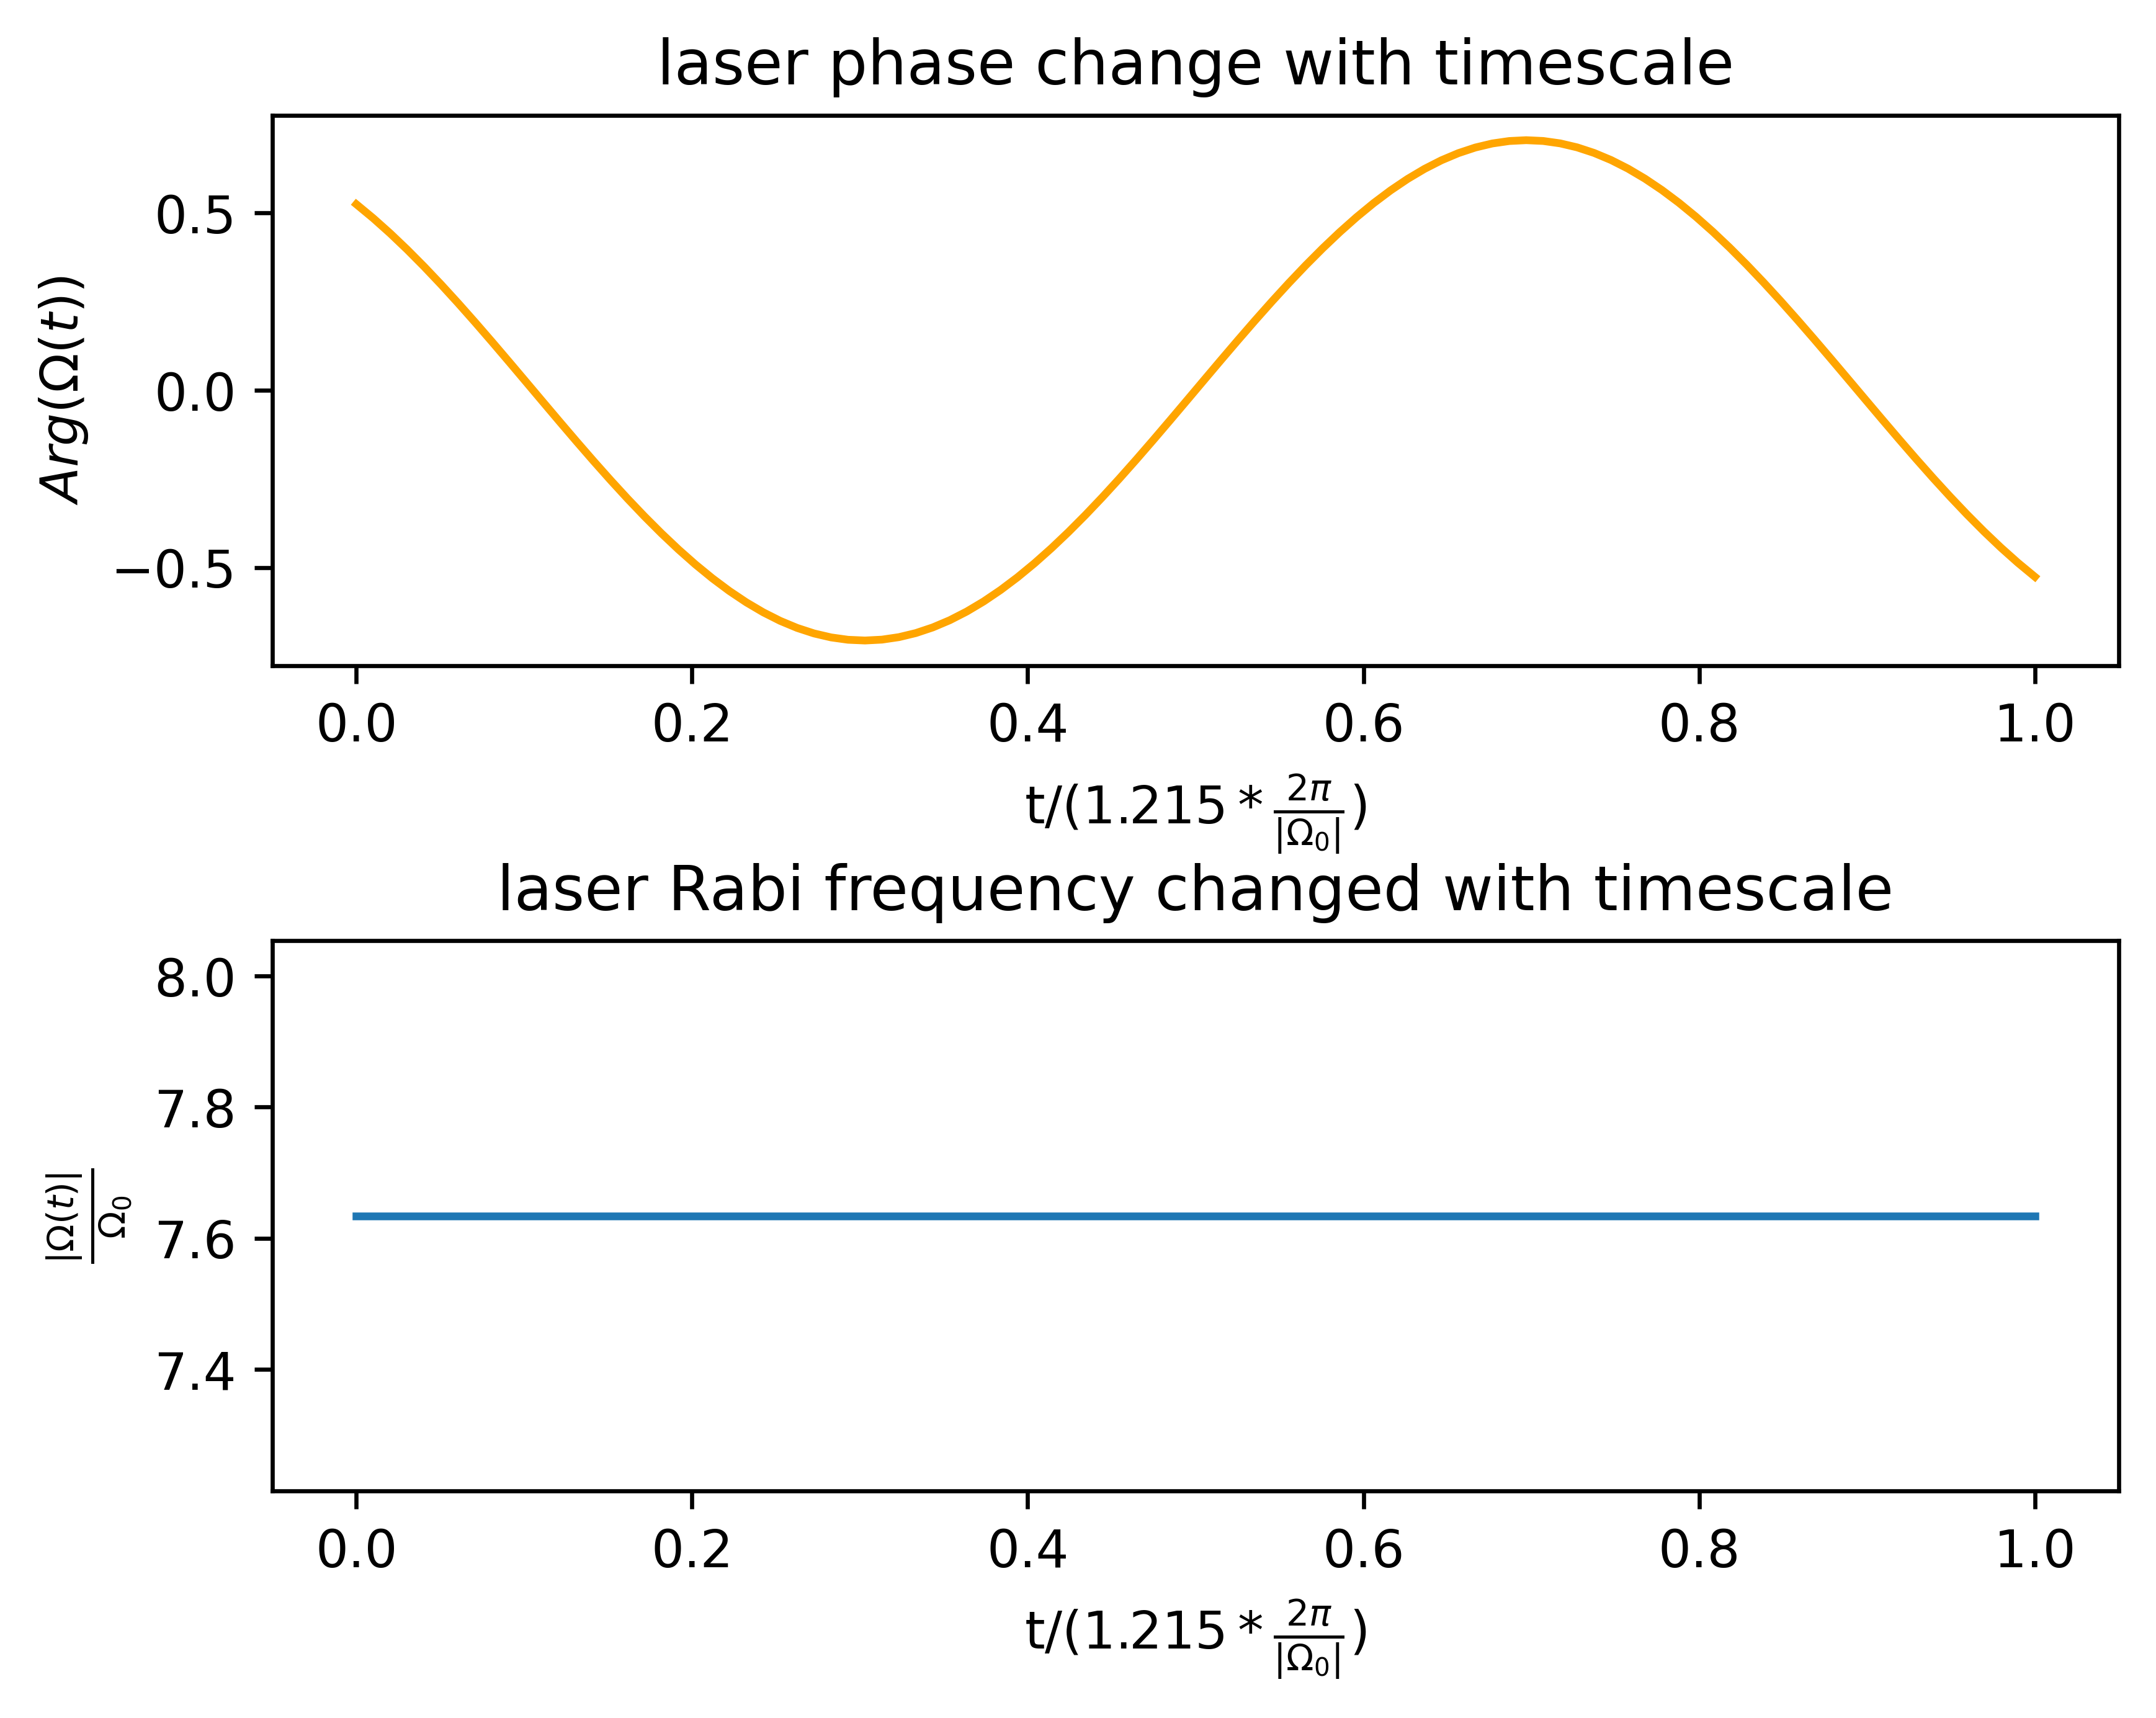
\includegraphics[height=5cm,width=6cm]{Figures/phaseconti_ws.png}
\hspace{0.5in}
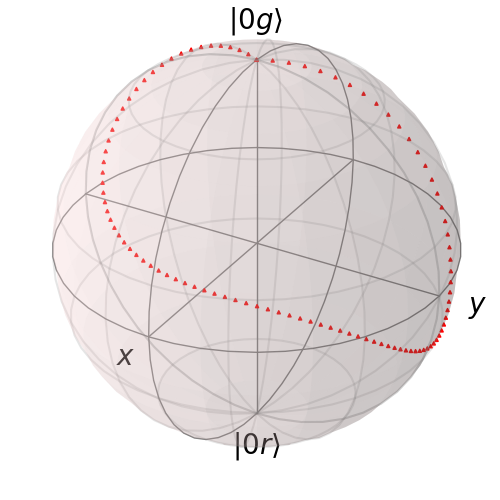
\includegraphics[height=4cm,width=4cm]{Figures/phaseconti_10.png}
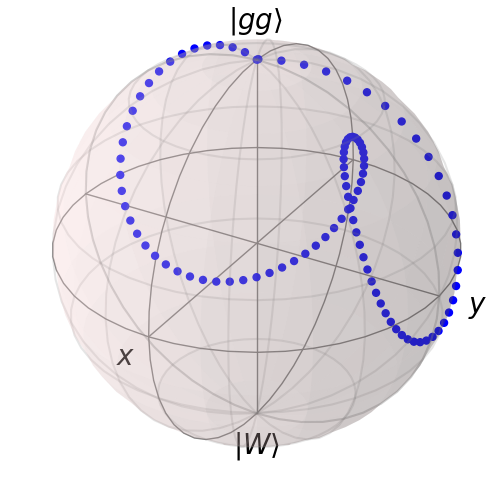
\includegraphics[height=4cm,width=4cm]{Figures/phaseconti_11.png}
\caption{The trace of the quantum state on the Bloch sphere of the time-optimal protocol. }
 \label{fig:anta-time-optimal}
\end{figure}

\paragraph*{Error-robust pulses---\!\!\!}
Time-optimal gate is the fastest gates, however, not robust to many noise like laser intensity noise, laser phase noise, stark-shift and Doppler effects due to atom temperature. Through pertubation theory, ones could design protocols that robust to these errors. In this section we follow the optimization tasks by Jandura \emph{et.al.}~\cite{PRXQuantum.4.020336} . 

First we consider the laser ampitude noise, which introduce an uncertainty $(1 + \varepsilon)\Omega_{\max}$ to the Rabi-frequency. The Hamiltonian then became:
\begin{align}\label{eq:twoqubit_Ham_withblockade_ampnoise}
    H_{q}^{\varepsilon}(t)&=(1 + \varepsilon)H_{q}(t).
\end{align}
The evolution of the state writes $\psi_q = \psi^{(0)}_q + \varepsilon\psi^{(1)}_q + \mathcal{O}(\varepsilon^2)$  and satisfied:
\begin{align}
    i\hbar \partial_t \ket{\psi_q^{(0)}} &= H_q(t)\ket{\psi_q^{(0)}},\\
     i\hbar \partial_t \ket{\psi_q^{(1)}} &= H_q(t)\ket{\psi_q^{(1)}}+H_q(t)\ket{\psi_q^{(0)}}.
\end{align}
For $q = \{01,11\}$, We solve the correlated Schrodinger equation and calculate:
\begin{align}
    J = 1 - \frac{1}{20} (|1 + 2a_{01} + a_{11}|^2 + |a_{11}|^2 + 2|a_{01}|^2 + 1) + \sum_{q = 01,10,11} \langle \psi_q^{(1)} | \psi_q^{(1)} \rangle,
\end{align}
where $a_{q} = \langle q|\psi_{q}^{(0)}(T)\rangle$. 
The value $J$ again became a function of sliced phase function $\{\phi(t_i)\}$ and could be minimized to give a Amplitude-noise Robust(AR) pulses.

 \subsubsection{Two photon process}
In protocols of Control-Z gate, the decreasing of the gate time will not only speed up the computation but also mitigate the decay error on the Rydberg states. 
However, For most one-photon process of the the Rydberg excitation, the frequency of the laser is high thus hard to increase the intensity. 
Considering one atom with energy level $\ket{r}, \ket{e}$ and $\ket{g} = \ket{1}$. Two laser light with Rabi requency $\Omega_1$ and $\Omega_2$ are imposed. The Hamiltonian is then written as:
\begin{align}
    H &= \hbar \omega_r \proj{r} + \hbar \omega_e \proj{e} +\hbar \omega_g \proj{g}  + \hbar \Omega_1(t) \cos[(\omega_e - \omega_g -\Delta)t + \phi_1(t)]\ket{g}\bra{e} + c.c. \\
    &+\hbar \Omega_2(t) \cos[(\omega_r - \omega_e +\Delta -\delta)t + \phi_2(t)]\ket{e}\bra{r} + c.c..
    \label{eq:two_photon_H}
\end{align}
Here we use positive $\delta$ and $\Delta$ to represent red-detuning of the $g \to e$ transition and $e \to r$ transition. In the case of $^{87}Rb$, $\Omega_1 =\Omega_{420}, \Omega_2= \Omega_{1013}$. We keep $\Omega_{1013}$ unchanged and use an arbitrary waveform generator that allows for arbitrary amplitude, frequency, and phase control which simultaneously drives two $420~nm$ AOMs in a tandem configuration and maps the RF waveform onto the $420~nm$ light\cite{Evered_2023}.

We consider the time-dependent unitary transition:
\begin{align}
    U(t) = e^{i\omega_g t \proj{g} + i(\omega_e - \Delta)t \proj{e} + i(\omega_r - \delta)t \proj{r}},
\end{align}
under which the Hamiltonian became:
\begin{align}
\label{eq:Lamman-two-photon}
    H' &= \hbar \delta \proj{r} + \hbar \Delta \proj{e} + \frac{\hbar \Omega_1(t) e^{i \phi_1(t)}}{2} \ket{g}\bra{e} + c.c.  \notag \\
    & \quad \quad +\frac{\hbar \Omega_2(t) e^{i \phi_1(t)}}{2} \ket{e}\bra{r} + c.c.
\end{align}
For two atoms inside the Rydberg radius, the Hamiltonian became:
\begin{align}
    H'_{\rm tot} &=\sum_{i = 1,2} \hbar \delta \proj{r}_i + \hbar \Delta \proj{e}_i + \frac{\hbar \Omega_1(t) e^{i \phi_1(t)}}{2} \ket{g}\bra{e}_i + c.c.  \notag \\
    &\quad \quad +\frac{\hbar \Omega_2(t) e^{i \phi_1(t)}}{2} \ket{e}\bra{r}_i + c.c. + B_{12} \ket{rr}\bra{rr}.
\end{align}
This Hamiltonian again form two subspace in the two-atoms Hilbert space. One,denoted as $\mathcal{H}_{0g}$ , begins from $\ket{0g}$ and spaned by $\{0g, 0e,0r\}$ and another subspace $\mathcal{H}_{gg}$ begins from $\ket{gg}$ and spaned by $\{gg,(ge+eg)/\sqrt{2},ee,(gr+rg)/\sqrt{2},(er+re)/\sqrt{2}\}$. The Hamiltonian in these two subspace are also list below:
\begin{align}
    H'_{tot,0g}/\hbar = 
    \begin{pmatrix}
        0 & \tilde\Omega_1(t)/2 & 0 \\
        \tilde\Omega_1^*(t)/2 &  \Delta & \tilde\Omega_2(t)/2\\
        0 & \tilde\Omega_2^*(t)/2 &   0
    \end{pmatrix}
\end{align}
\begin{align}
    H'_{tot,gg}/\hbar = 
    \begin{pmatrix}
        0 & \sqrt{2}\tilde\Omega_1(t)/2 & 0&0&0 \\
        \sqrt{2}\tilde\Omega_1^*(t)/2 &  \Delta &  \sqrt{2}\tilde\Omega_1(t)/2&\tilde\Omega_2(t)/2&0\\
        0 &  \sqrt{2}\tilde\Omega_1^*(t)/2 &   2\Delta&\sqrt{2}\tilde\Omega_2(t)/2&0 \\
        0&\tilde\Omega_2^*(t)/2&\sqrt{2}\tilde\Omega_2^*(t)/2&\delta&\tilde\Omega_1(t)/2 \\
        0&0&0&\tilde\Omega^*_1(t)/2&\Delta + \delta \\
    \end{pmatrix}
\end{align}
\subsection{Erasure conversion scheme}
In the last section, we ignore the fact that atoms has finite decay rate. For those decay on dark states, it  equivalence 
\subsection{Noise simulations for Control-Z Gate}
In this section, we give the real simulation of $\text{CPHASE}$ gate used by Evered \emph{et.al.}~\cite{Evered_2023}, based on $^{87}Rb$ atoms.
\subsubsection{Hamiltonian analysis}
\begin{figure}[!htbp]
    \centering
    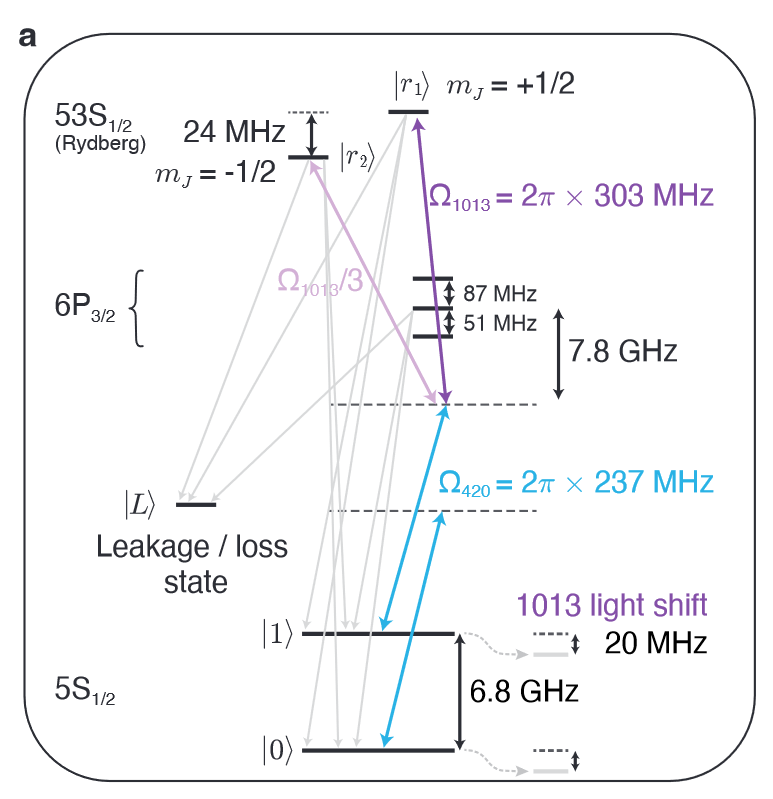
\includegraphics[width=0.5\linewidth]{Figures/Real_Rb_Elevel.png}
    \caption{Related energy level of $^{87}{Rb}$. Atoms is excited to Rydberg state through two lasers with $1013\text{nm}$ wave-length and $420\text{nm}$ wave-length. }
    \label{fig:Real_Rb_Elevel}
\end{figure}
We sequentially choose the basis states $\ket{0}: \{5S_{1/2}, F = 1, m_F = 0\}$ and $\ket{1}: \{5S_{1/2}, F = 2, m_F = 0\}$ as the qubit space. The intermediate states, obtained through $420\text{nm}$  $\sigma_+$ light with large red-detuning $\Delta = 7.8 \text{GHz}$, consist of three levels split by hyperfine structure:
\[\ket{2}, \ket{3}, \ket{4} = \{6P_{3/2}, F = 1, 2, 3, m_F = +1\}\]
For Rydberg levels, the dominant term in the electronic Hamiltonian is $\vec{B} \cdot (\vec{L} + \vec{S})$, far greater than the coupling term of nuclear spin $\vec{I} \cdot (\vec{L} + \vec{S})$. Viewing nuclear spin coupling as a perturbation, the unperturbed Hamiltonian commutes with $L^2$, $S^2$, $J^2$, and $J_z$, hence the choice of the $m_j$ representation.
We aim to excite atoms to $\ket{5} = \{53S_{1/2}, m_j = +1/2\}$ using $1013\text{nm}$ $\sigma_-$ light. However, due to the presence of not only components with $\{6P_{3/2}, m_j = +3/2\}$ in the intermediate state but also components with $\{6P_{3/2}, m_j = +1/2\}$, atoms will inevitably be excited to $\ket{6} = \{53S_{1/2}, m_j = -1/2\}$. In the experiment, a magnetic field is applied to induce a $24$ MHz splitting between $\ket{5}$ and $\ket{6}$ to mitigate this effect.

According to the $CG$-coefficient, we are able to transfer from the superfine-basis into $\{L^2,S^2,J^2,I^2,m_J,m_I\}$ basis.
\begin{align*}
\ket{0} &= 1/\sqrt{2}\left[-\{m_j = 1/2, m_I = -1/2\} + \{m_j = -1/2, m_I = 1/2\}\right] \\
\ket{1} &= 1/\sqrt{2}\left[\{m_j = 1/2, m_I = -1/2\} +\{m_j = -1/2, m_I = 1/2\}\right] \\
\ket{2} &= \sqrt{\frac{3}{10}}\{m_j = 3/2, m_I = -1/2\} -\sqrt{\frac{2}{5}}\{m_j = 1/2, m_I = 1/2\} +\sqrt{\frac{3}{10}} \{m_j = -1/2, m_I = 3/2\}\\
\ket{3} &= \frac{1}{\sqrt{2}}\{m_j = 3/2, m_I = -1/2\} -\frac{1}{\sqrt{2}} \{m_j = -1/2, m_I = 3/2\} \\
\ket{4} &= \frac{1}{\sqrt{5}}\{m_j = 3/2, m_I = -1/2\} +\sqrt{\frac{3}{5}}\{m_j = 1/2, m_I = 1/2\} +\frac{1}{\sqrt{5}} \{m_j = -1/2, m_I = 3/2\}\\
\ket{5}&= \{53S_{1/2},m_j = +1/2\}, \ket{6}= \{53S_{1/2},m_j = -1/2\}
\end{align*}
We consider the $\Omega_{420}$ labeled in Figure~\ref{fig:Real_Rb_Elevel} as the coupling coefficient:
\[
\Omega_{420} =: \frac{\langle \{5S_{1/2}, m_j = 1/2, m_I = -1/2\}| e\vec{E}_+\cdot \vec{r}| \{6P_{3/2}, m_j = 3/2, m_I = -1/2\}\rangle}{\sqrt{2}\hbar}
\]
Defining:
\[
\frac{\langle \{5S_{1/2}, m_j = -1/2, m_I = 1/2\}| e\vec{E}_+\cdot \vec{r}| \{6P_{3/2}, m_j = 1/2, m_I = 1/2\}\rangle}{\sqrt{2}\hbar} = \gamma \Omega_{420}
\]
Using the rotating wave approximation, we can further express:
\begin{align*}
\langle 2| H | 1 \rangle &= \text{CG}(3/2,3/2,3/2,-1/2,1,1)\Omega_{420}/2 +\text{CG}(3/2,1/2,3/2,1/2,1,1) \gamma \Omega_{420}/2 \\
&=\sqrt{0.3}\Omega_{420}/2 - \sqrt{0.4}\gamma \Omega_{420}/2 \\
\langle 3| H | 1 \rangle &= \text{CG}(3/2,3/2,3/2,-1/2,2,1)\Omega_{420}/2 +\text{CG}(3/2,1/2,3/2,1/2,2,1) \gamma \Omega_{420}/2 \\
&=\sqrt{0.5}\Omega_{420}/2 \\
\langle 4| H | 1 \rangle &= \text{CG}(3/2,3/2,3/2,-1/2,3,1)\Omega_{420}/2 +\text{CG}(3/2,1/2,3/2,1/2,3,1) \gamma \Omega_{420}/2 \\
&=\sqrt{0.2}\Omega_{420}/2 + \sqrt{0.6}\gamma \Omega_{420}/2 
\end{align*}
Similarly, the action of $\Omega_{1013}$ can be expressed analogously. Define:
\begin{align}
\Omega_{1013} &=: \langle\{53S_{1/2},m_j = +1/2\}|e\vec{E}_-\cdot \vec{r} |\{6P_{3/2},m_j = 3/2\}\rangle \\
\beta \Omega_{1013} &=: \langle\{53S_{1/2},m_j = -1/2\}|e\vec{E}_-\cdot \vec{r} |\{6P_{3/2},m_j = 1/2\}\rangle
\end{align}
\begin{align*}
\langle 5| H | 2 \rangle &= \text{CG}(3/2,3/2,3/2,-1/2,1,1)\Omega_{1013}/2 = \sqrt{0.3}\Omega_{1013}/2   \\
\langle 5| H | 3 \rangle &= \text{CG}(3/2,3/2,3/2,-1/2,2,1)\Omega_{1013}/2= \sqrt{0.5}\Omega_{1013}/2   \\
\langle 5| H | 4 \rangle &= \text{CG}(3/2,3/2,3/2,-1/2,3,1)\Omega_{1013}/2= \sqrt{0.2}\Omega_{1013}/2  \\
\langle 6| H | 2 \rangle &= \text{CG}(3/2,1/2,3/2,1/2,1,1) \beta \Omega_{1013}/2= -\sqrt{0.4}\beta\Omega_{1013}/2  \\
\langle 6| H | 3 \rangle &= \text{CG}(3/2,1/2,3/2,1/2,2,1) \beta \Omega_{1013}/2= 0  \\
\langle 6| H | 4 \rangle &= \text{CG}(3/2,1/2,3/2,1/2,3,1) \beta \Omega_{1013}/2= \sqrt{0.6}\beta\Omega_{1013}/2 \\
\end{align*}
The specific value of $\gamma,\beta$ can be obtained by integrating the wave function. Here, we directly use Arc to obtain the result: $\gamma = \beta = \sqrt{1/3}$.
For simplicity,  we denote $\bra{i}H\ket{j} =: H_{ij}$. The process in Figure~\ref{fig:Real_Rb_Elevel} is stimulated Raman transitions concerning three intermediate states $\{\ket{2},\ket{3},\ket{4}\}$. Noted that due to the detuning between two Rydberg states, we ignore the influence of state $\ket{6}$. We then write the Schrodinger equation according to Eq.~\eqref{eq:Lamman-two-photon}.
\begin{align}
    i\hbar \partial_t \psi_i &= (H_{i1} \psi_1 + H_{i5}\psi_5) + \Delta \psi_i \quad \forall~i = 2,3,4, \\ 
    i\hbar\partial_t \psi_5 &= \sum_{i = 2,3,4} H_{5i} \psi_i,\\
    i\hbar\partial_t \psi_1 &=  \sum_{i = 2,3,4} H_{1i} \psi_i.
\end{align}
We can adiabatically eliminate the intermediate states through setting $\partial_t \psi_i = 0,~\forall~i = 3,4,5$. This then give the effective two-level transition between state $\ket{1}$ and state $\ket{5}$.
\begin{align}
    i\hbar\partial_t \psi_5&=  -\sum_{i = 2,3,4} \frac{|H_{5i}|^2}{\Delta} \psi_5 - \left(\sum_{i = 2,3,4} \frac{H_{i1} H_{5i}}{\Delta}\right) \psi_1  ,\\
      i\hbar\partial_t \psi_1 &=  -\sum_{i = 2,3,4} \frac{|H_{1i}|^2}{\Delta} \psi_1 - \left(\sum_{i = 2,3,4} \frac{H_{i5} H_{1i}}{\Delta}\right) \psi_5  .
\end{align}
Then the effective light-shift and the effective Rabi frequency write:
\begin{align}
    \Delta_{\text{eff,5}} &= -\sum_{i = 2,3,4} \frac{|H_{5i}|^2} {\Delta} = -\frac{\Omega_{1013}^2}{4\Delta},\\
     \Delta_{\text{eff,1}} &= -\sum_{i = 2,3,4} \frac{|H_{1i}|^2} {\Delta} =- \frac{4}{3} \frac{\Omega_{420}^2}{4\Delta}\\
    \Omega_{\text{eff}} &= -2\frac{\sum_{i = 2,3,4} H_{i1} H_{5i}}{\Delta} = -\frac{\Omega_{1013}\Omega_{420}}{2\Delta}
\end{align}
From the resonance condition, we also find resonance proportion;
\begin{align}
    \Omega_{1013}/\Omega_{420} = (\sqrt{0.3} - \sqrt{\frac{0.4}{3}})^2+(\sqrt{0.2} + \sqrt{\frac{0.6}{3}})^2 +0.5 = \frac{4}{3}
\end{align}
Given these result, any real gate strategy that use constant $1013\text{nm}$ laser with Rabi frequency $\Omega_{1013}$ and a time-dependent $460\text{nm}$ laser with $\tilde\Omega_{420}(t) = \Omega_{420}(t) e^{i\phi_{420}(t)}$ correspond to a two-level system gate strategy satisfied:
\begin{align}
    \Omega(t) &= -\frac{\Omega_{1013}\Omega_{420}(t)}{2\Delta} \\
    \phi(t) &= \phi_{420}(t) +\frac{\Omega_{\text{1013}}^2}{4\Delta} t - \frac{4}{3} \int dt \frac{\Omega_{\text{420}}^2(t)}{4\Delta}
\end{align}
With these equations, ones could transfer any optimized gate-protocol to this real system and simulate its error source and error distributions. The gate-protocol is given as functions $f(x),\psi(x)$  for $x\in (0,1)$. If we further given $\Omega_{1013}, \Delta$ and maximum value of $420\text{nm}$ laser $\Omega_{\text{max}}$ , we correspond this to a real protocol:
\begin{align}
    \Omega_{420}(t) &= - \frac{\Omega_{\max}}{f_m} f(t/T), \\
    \phi_{420}(t) &= \phi(t/T) - \frac{\Omega_{1013}^2}{4\Delta} t + \frac{\Omega_{\max}^2 T}{3\Delta f_m^2}\int_{x = 0}^{x =  t/T} dx f^2(x), \\
    \text{where,}~ T &= \frac{2\Delta f_m}{\Omega_{1013} \Omega_{\max}}.
\end{align}

\subsubsection{Laser noise analysis}
Through the phase and intensity of the lasers are stabilized through technical methods such as Pound-Drever-Hall Feedforward~\cite{chao2023pounddreverhall}, they still exists.
The effect of such noises could be represented as a random function $\phi_{n}(t)$ and $\Omega_{n}(t)$. We first consider the phase noise only. The two-photon process Hamiltonian in Eq.~\eqref{eq:two_photon_H} now became:
\begin{align*}
    H &= \hbar \omega_r \proj{r} + \hbar \omega_e \proj{e} +\hbar \omega_g \proj{g}  \\
    & \quad \quad + \hbar \Omega_1(t) \cos[(\omega_e - \omega_g -\Delta)t + \phi_1(t) +  \phi_{1n}(t)]\ket{g}\bra{e} + c.c. \\
    & \quad \quad +\hbar \Omega_2(t) \cos[(\omega_r - \omega_e +\Delta -\delta)t + \phi_2(t) +  \phi_{2n}(t)]\ket{e}\bra{r} + c.c..
\end{align*}
It is more convenient to move the phase noise term into the diagonal terms as a time dependent detuning $\delta(t) = -\dot{\phi}(t)$ . Thus we consider the transition:
\begin{align}
    U(t) = exp\left(i\omega_g t \proj{g} + i[(\omega_e - \Delta)t + \phi_{1n}(t)] \proj{e} + i[(\omega_r - \delta)t + \phi_{2n}(t) + \phi_{1n}(t)] \proj{r}\right),
\end{align}
If the noise is small, $\dot{\phi}_{2n}(t),\dot{\phi}_{1n}(t) \ll \omega_r,\omega_e,\omega_g$ , we concludes:
\begin{align}
H'_{\rm tot} &= i\hbar \frac{dU}{dt} U^\dagger + UHU^\dagger \\
&= \hbar (\delta -\dot{\phi}_{1n}(t)-\dot{\phi}_{2n}(t) ) \proj{r} + \hbar (\Delta - \dot{\phi}_{1n}(t)) \proj{e}   \notag \\
&\quad \quad + \frac{\hbar \Omega_1(t) e^{i \phi_1(t)}}{2} \ket{g}\bra{e} + c.c. +\frac{\hbar \Omega_2(t) e^{i \phi_1(t)}}{2} \ket{e}\bra{r} + c.c. 
\end{align}
It is find that the full phase-noise model is well described by a Gaussian servo bump combined with white noise~\cite{PhysRevA.107.042611}. The power spectral density can be expressed as:
\[S_{\delta \nu}(f) = h_0 + \frac{s_g f_g^2}{\sqrt{8\pi} \sigma_g} e^{\frac{-(f - f_g)^2}{2\sigma_g^2}} + \frac{s_g f_g^2}{\sqrt{8\pi} \sigma_g}  e^{\frac{-(f + f_g)^2}{2\sigma_g^2}}\]
When \(s_g = 0\), it becomes white noise. Additionally, there may exist multiple Gaussian bumps. 
Given the power spectral density, the noise can be reproduced using frequency mixing with uniformly random phases. If the power spectral density of the phase noise is known as \(S_{\phi}(f)\), it can be set as:
\[\phi(t) = \sum_{j = 1}^{\infty} 2 \sqrt{S_{ \phi}(f_j) \Delta f} \cos (2\pi f_j t + \varphi_j )\]
where \(\varphi_i\) is uniformly selected random variables from the interval \([0,2\pi]\). The derivative of the above random function is:
\begin{align}
\frac{d\phi(t)}{dt} &= -\sum_{j = 1}^{\infty} 4\pi f_j \sqrt{S_{ \phi}(f_j) \Delta f} \sin (2\pi f_j t + \varphi_j ) \\
&= -\sum_{j = 1}^{\infty} 4\pi\sqrt{S_{ \delta\nu}(f_j) \Delta f} \sin (2\pi f_j t + \varphi_j ) 
\end{align}
where the relationship \(S_{ \delta\nu}(f) = f^2 S_{ \phi}(f)\) is utilized.

To get confident about the simulation of phase noise, we reproduced the $\pi$-pulase and $2\pi$-pulse fidelity under different noise center $f_g$ . To be specific, we set a laser with Rabi frequency \(\Omega = 2\pi \times1 \text{ MHz}\), and set \(h_0 = 0 \text{ Hz}\), \(f_g \in (0.1,4) \times \frac{\Omega}{2\pi}\), \(\sigma_g = 1400 \text{ Hz}\), \(s_g = \frac{\sqrt{8\pi } \sigma_g h_g}{f_{g0}^2}\), where \(h_g = 1100\) and \(f_{g0} = 10^6\). 
\begin{figure}[!hbtp]
    \centering
    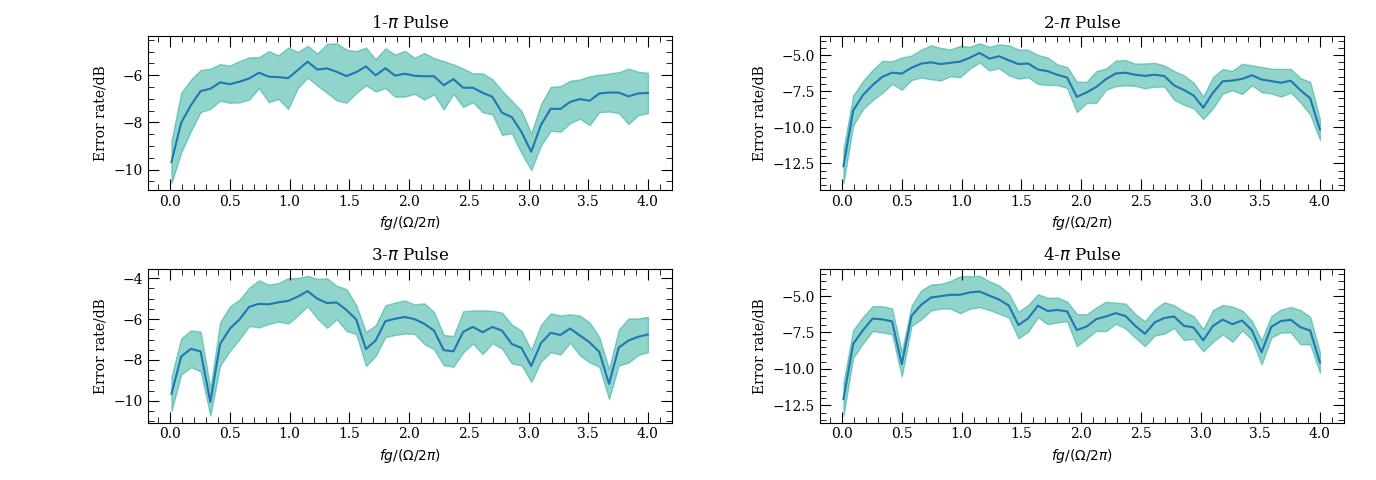
\includegraphics[width=1\linewidth]{Figures/servo_btm.png}
    \caption{Betchmark of our gate simulation result. We choose to plot how the $n\pi$ pulse fidelity changed according to the shift of servo-bump noise centre, $f_g$. This result corresponds to the previous research by Jiang \emph{et.al.}~\cite{PhysRevA.107.042611} .}
    \label{fig:benchmarking_servonoise}
\end{figure}

In our $^{87}Rb$ simulation, we use the noise data of a 1040 nm solid-state Ti:Sa laser which was locked to a reference cavity with linewidth of approximately 5 kHz using the Pound-Drever-Hall method. It is experimentally measured by Jiang \emph{et.al.}~\cite{PhysRevA.107.042611} .
\begin{align}
    S_{\delta \nu}(f) = 13 +25 [e^{\frac{-(f/1000 - 130)^2}{2\times 18^2}} + e^{\frac{-(f/1000 + 130)^2}{2\times 18^2}}] + 2000 [e^{\frac{-(f/1000 - 234)^2}{2\times 1.5^2}} + e^{\frac{-(f/1000 + 234)^2}{2\times 1.5^2}}]
\end{align}


\subsubsection{Gate error simulation}
To analysis the equivalent Pauli error rate and loss error rate, 

In many protocols, Rydberg state serves as an important strong interacting state to implement interaction between different atoms. However, the instability of Rydberg state also cause many error channels.
The error is introduced through many channels. Rydberg states first are sensitive to environment black-body radiation and could easily collapse as illustrated in Section~\ref{sec:error_atoms}. 
\paragraph*{BBR transition error---\!\!\!}
The Kraus operators of BBR error channel is presented below~\cite{PhysRevX.12.021049}
\begin{align}
M_{r'} = P_{r'} \ket{r'}\bra{1}, \quad M_0 = \sqrt{1 - \sum_{r'}P_{r'}} \proj{1} + \sum_{n \neq 1}\proj{n}.    
\end{align}
The parameter $P_{r'}$ is determined by the BBR transition rate between Rydberg state $\ket{r}$, that used to mediate two qubits interaction, and another Rydberg state $\ket{r'}$. They have narrow energy gap thus sensitive to the back-ground black-body radiations. 

\paragraph*{Spontaneous emission error---\!\!\!}
Atoms at Rydberg state has possibility to decay into the qubit state $\ket{1},\ket{0}$ and other non-computational basis $\ket{f}$. This spontaneous emission process combined with the driving light between Rydberg state and $\ket{1}$ state will cause channel below~\cite{PhysRevX.12.021049}:
\begin{align}
    M_0 = \proj{r} + \alpha \proj{1} + \beta \proj{0}, \quad M_r = p_r \ket{r}\bra{1}, \\
    \quad M_1 = p_1\proj{1}, \quad M_2 = p_2 \proj{0},M_f = p_f\ket{f}\bra{1}. \notag
\end{align}

\paragraph*{Real simulation---\!\!\!}
To strictly consider the impact of spontaneous emission of the two atoms and laser noise effect, we need to rigorously solve the master equation as follows:
\begin{align}
\frac{\partial \rho}{\partial t} &= \frac{-i}{\hbar} [H(t), \rho] + \sum_\mu ( M_\mu \rho M_\mu^\dagger - \frac{1}{2} M_\mu^\dagger M_\mu \rho - \frac{1}{2} \rho M_\mu^\dagger M_\mu ) \\
&=\frac{-i}{\hbar} (H_{\text{eff}}\rho - \rho H_{\text{eff}}^\dagger)+ \sum_\mu M_\mu \rho M_\mu^\dagger , \quad H_{\text{eff}}(t) = H(t) - \sum_{\mu}i\frac{\hbar}{2} M_\mu^\dagger M_\mu
\end{align}
 We first noticed that for single atom,
\begin{align}
M_{j \to i} &= \ket{i}\!\bra{j} \sqrt{\Gamma_{ji}},\\
 \sum_{i,j}M_{j \to i}^\dagger M_{j \to i} &= \sum_{i,j}\ket{j}\!\bra{j} \Gamma_{ji} = \sum_{j} \Gamma_j \ket{j}\!\bra{j},
\end{align}
where $\Gamma_j$ depends only on the lifetime of level $j$. For the spontaneous emission of two atoms, $M_{\mu} = \{M_{j \to i} \otimes \mathbb{I},~ \mathbb{I} \otimes M_{j \to i},~ M_{j \to i} \otimes M_{j' \to i'}\}$. This means that:
\begin{align}
    H_{\text{eff}}(t) &\approx H_{s}(t) \otimes H_{s}(t) -i\frac{\hbar}{2} \sum_{j} \Gamma_j \ket{j}\!\bra{j} \otimes \mathbb{I} -i\frac{\hbar}{2}   \mathbb{I} \otimes \sum_{j} \Gamma_j \ket{j}\!\bra{j} \\
    &\approx \left( H_{s}(t)-i\frac{\hbar}{2} \sum_{j} \Gamma_j \ket{j}\!\bra{j} \right) \otimes \left( H_{s}(t)-i\frac{\hbar}{2} \sum_{j} \Gamma_j \ket{j}\!\bra{j} \right)
\end{align}
We then define the propagator of $H_{\text{eff}}(t)$ as $U_{\text{eff}}(t)$ and $\sigma = U^{-1}_{\text{eff}}(t)\rho U^{-1,\dagger}_{\text{eff}}(t) $, which satisfied:
\begin{align}
    \frac{d \sigma}{dt} =U^{-1}_{\text{eff}}(t) \left[\sum_{\mu} M_\mu \rho M_\mu^{\dagger}\right] U_{\text{eff}}^{-1,\dagger}(t)
\end{align}
Again through keep the linear term of  $\Gamma_{ji}$ only, we concludes that:
\begin{align}
    \sigma(t_0) = \sigma(0) + \int_0^{t_0} \!dt~U^{-1}_{\text{eff}}(t)  M_\mu U_{\text{eff}}(t)  \sigma(0) U^{\dagger}_{\text{eff}}(t)  M_{\mu}^\dagger U_{\text{eff}}^{-1,\dagger}(t) + \mathcal{O}(\Gamma^2)
\end{align}
We then conclude that the original state $\rho(t)$ evolve as:
\begin{align*}
    \rho(t_0) &=  U_{\text{eff}}(t_0) \rho(0)  U^{\dagger}_{\text{eff}}(t_0) +\sum_{\mu}U_{\text{eff}}(t_0)  \int_0^{t_0} \!dt~U^{-1}_{\text{eff}}(t)  M_\mu U_{\text{eff}}(t)  \rho(0) U^{\dagger}_{\text{eff}}(t)  M_{\mu}^\dagger U_{\text{eff}}^{-1,\dagger}(t) U^{\dagger}_{\text{eff}}(t_0)   \\
     &=U_{\text{eff}}(t_0) \rho(0)  U^{\dagger}_{\text{eff}}(t_0) +\sum_{u,v,j,i} \Gamma_{j \to i} \int_0^{t_0} d\tau U(\tau) \ket{i,v}\!\!\bra{i,u}U^{-1}(\tau) \bra{j,v} \rho^H_{\rho(0)}(t_0 - \tau) \ket{j,u}  + \text{Q.E.}\\
    &= U_{\text{eff}}(t_0) \rho(0)  U^{\dagger}_{\text{eff}}(t_0) +\sum_{u,v,j,i} \Gamma_{j \to i} \int_0^{t_0} d\tau \rho_{\ket{i}\!\bra{i} \otimes \ket{v}\!\bra{u}}^H(\tau) \bra{j,v} \rho^H_{\rho(0)}(t_0 - \tau) \ket{j,u} + \text{Q.E.} \\
    &= U_{\text{eff}}(t_0) \rho(0)  U^{\dagger}_{\text{eff}}(t_0)+ \sum_{j,i} \Gamma_{j \to i} \int_0^{t_0} d\tau \rho_{\rho(0)}^{H_\tau}(t_0)  + \text{Q.E.}
\end{align*}
Here $H_\tau$ is the same Hamiltonian evolution as $H$ but with a un-normalized measurement-and-replacement operation $\ket{i}\!\bra{j} \otimes \mathbb{I}$ (or  $\mathbb{I}\otimes\ket{i}\!\bra{j}  $ for another atom) inserted at time $\tau$.
Noticed that the input state $\rho(0)$ is restrained on the subspace spaned by states $\{\ket{mn}, m,n = 0,1\}$. The main decay effects stem from states $\{\ket{i},~ i = 2,3,4,5,6\}$ for intermediate states, Rydberg state and garbage Rydberg state. They could decay into the states $\{L_r,L_g,\ket{1},\ket{0}\}$, where $L_r, L_g$ is the leak states that includes other black-body radiation(BBR) interacting Rydberg states or ground states out of the computational basis.

We input the state $\ket{\phi(0)} = a\ket{00} + b\ket{01} + c\ket{10} + d \ket{11}$. The simulation of the 7-level Hamiltonian could give the full wave function at time $\tau$, which we denote:
\begin{align}
    \ket{\phi(\tau)} &=a\ket{00} + b \sum_{s \in \{1,\cdots 6\}} \beta_{s}(\tau) \ket{0 s} + c \sum_{s \in \{1,\cdots 6\}} \beta_{s}(\tau) \ket{ s0} \notag  \\
   &\quad\quad\quad  + d \sum_{s_1,s_2 \in \{1,\cdots 6\}} \alpha_{s_1 s_2}(\tau) \ket{s_1 s_2} .
\end{align}
Consider the quantum jump $\mathbb{I} \otimes \ket{L_g}\!\bra{2}$, we have:
\begin{align}
  (\mathbb{I} \otimes  \ket{L_g}\!\bra{2})\ket{\phi(\tau)} = d\sum_{s_1\in \{1,\cdots 6\}} \alpha_{s_1 2}(\tau) \ket{s_1 L_g} + b  \beta_{2}(\tau) \ket{0 L_g}.
\end{align}
Then this projected states evolve for the test time $t_0 - \tau$. For state with $s_1 = 0$, it will unchanged for the large detuning between $\ket{0L_g}$ state and the other states. For the other choice of $s_1$, state will transformed among states besides $\ket{0L_g}$ and finally all became state $\ket{11}$ for erasure conversion. Then we concludes that:
% \begin{align}
%     \rho_{\phi}^{H_\tau}(\tau) &= \ket{\Phi}\! \bra{\Phi}, \\
%     \text{where, ~} \ket{\Phi} &= d\sum_{s_1\in \{1,\cdots 6\}} \alpha_{s_1 2}(\tau) \ket{11} + b  \beta_{2}(\tau) \ket{0 1}
% \end{align}
% The some terms of the un-normalized density matrix are fast oscillating thus vanish under the integral from $[0, t_0]$. We concludes that:
\begin{align*}
    \int_0^{t_0} d\tau \rho_{\phi}^{H_\tau}(\tau) =d^2 \sum_{s_1\in \{1,\cdots 6\}}  \left(\int_0^{t_0} d\tau |\alpha_{s_1 2}(\tau) |^2 \right)\ket{11}\!\bra{11} + b^2  \left(\int_0^{t_0} d\tau |\beta_2(\tau)|^2 \right)\ket{01}\!\bra{01}
\end{align*}
This equation then tell us the channel has Kraus operators as:
\begin{align}
    M_{11 \to 11} &=\sqrt{\Gamma_{2 \to L_g} P_{\ket{11},\ket{2}}}\ket{11}\!\bra{11},\\
     M_{01 \to 01} &=\sqrt{\Gamma_{2 \to L_g} P_{\ket{01},\ket{2}}}\ket{01}\!\bra{01}.
\end{align}
Here $P_{\ket{11},\ket{2}}$ denotes the cumulative probability that one atoms is in state $\ket{2}$ with simulation input $\ket{11}$. Similar analysis could be applied on all possible quantum jump and give the full Kraus channel as below:
\begin{align*}
     M_{11 \to 11} &=\sqrt{\!\!\sum_{\substack{
     \{2,3,4,5,6\} \to \{L_g ,1\};\\
     \{5,6\} \to \{L_r\};
     }}\!\!\!\!\!\!2\Gamma_{j \to i} P_{\ket{11},\ket{j}}}\ket{11}\!\bra{11}, \quad
     M_{01 \to 01} =\sqrt{\!\!\sum_{\substack{
     \{2,3,4,5,6\} \to \{L_g ,1\};\\
     \{5,6\} \to \{L_r\};
     }}\!\!\!\!\!\!\Gamma_{j \to i} P_{\ket{01},\ket{j}}}\ket{01}\!\bra{01},\\
     M_{10 \to 10} &=\sqrt{\!\!\sum_{\substack{
     \{2,3,4,5,6\} \to \{L_g ,1\};\\
     \{5,6\} \to \{L_r\};
     }}\Gamma_{j \to i} P_{\ket{01},\ket{j}}}\ket{10}\!\bra{10},\quad
     M_{11 \to 10} =\sqrt{\!\!\!\sum_{ \substack{\{2,3,4,5,6\} \to \{0\};
     }}\Gamma_{j \to i} P_{\ket{11},\ket{j}}}\ket{10}\!\bra{11},\\
     M_{11 \to 01} &=\sqrt{\!\!\!\sum_{ \substack{\{2,3,4,5,6\} \to \{0\};
     }}\Gamma_{j \to i} P_{\ket{11},\ket{j}}}\ket{01}\!\bra{11},\quad
      M_{10 \to 00} =\sqrt{\!\!\!\sum_{ \substack{\{2,3,4,5,6\} \to \{0\};
     }}\Gamma_{j \to i} P_{\ket{10},\ket{j}}}\ket{00}\!\bra{10},\\
      M_{01 \to 00} &=\sqrt{\!\!\!\sum_{ \substack{\{2,3,4,5,6\} \to \{0\};
     }}\Gamma_{j \to i} P_{\ket{01},\ket{j}}}\ket{00}\!\bra{01}.
\end{align*}
Another important information of two-qubit gate is the probability that end up with the leakage ground states, leakage Rydberg states and $\ket{0}, \ket{1}$ space.  

% Monte-Carlo Wave Function(MCWF) method regards the evolution of the master equation as a probabilistic process. With probability $1- \delta p$, it evolves with the non-Hermitian Hamiltonian $H_{\text{eff}}$, and with probability $\delta p$, it evolves according to the rule $\ket{\psi} \to M_{\mu} \ket{\psi}$ (note that it is a classical probability mixture, not a superposition state).Thus, it is sufficient to insert $\sum_{i,j}M_{j \to i}^\dagger M_{j \to i}$ into the Hamiltonian of a single atom to characterize the possibility of decay from $j \to i$:

%  Assuming that the state after spontaneous emission will not be re-excited but will remain unchanged in the original level, we can simplify the treatment as follows:

% \begin{itemize}
% \item At $t = T$, evolve the system with the effective Hamiltonian obtained above to obtain the normalized trajectory $\ket{\psi(t)}$ and the unnormalized final state $\ket{\psi}_{\text{end}} = \ket{\psi(T)}$, where the probability of being in this state is its modulus squared, $p = |\bra{\psi_{\text{end}}} \psi_{\text{end}}\rangle|^2$.
% \item Additionally, there is a probability of single qubit decay. Double qubit decay is a second-order small quantity and can be ignored. The probability of any qubit decaying from state $\ket{j}$ can be approximately calculated as:
% \begin{align}
% p_{j} &= \sum_{i}\int_{t = 0}^T dt  ||M_{j \to i} \otimes \mathbb{I}  \ket{\psi(t)}||^2 = \sum_{i} \Gamma_{ji}\int_{t = 0}^T dt  \langle \ket{j}\!\bra{j} \otimes \mathbb{I} \rangle_{\psi(t)}
% \end{align}
% \end{itemize}
% This probability only depends on the lifetime of state $j$ . Thus in this way, ones get the source information of the gate noise, that is, the probability of intermediate state decay and Rydberg state decay at the end of gate protocol and the. 

\section{QECC with surface codes}
\begin{definition}{Quantum error correction code(QECC)}
    A $k$-dimensional quantum error correcting code for a finite set of errors $ \mathbb{E} := \{ E_a \}_{a \in \Lambda}$ embedded in a $N$-dimensional Hilbert space $\mathcal{H}$ is a pair $(\mathcal{S}, \mathcal{R})$ where $\mathcal{Q}$ is a $K$-qubit subspace of $\mathcal{H}$ and $\mathcal{R}$ is a CPTP map $\mathcal{H} \to  \mathcal{H} $ such that $\forall \rho$ as a density matrix of $\mathcal{Q}$ and $\forall E_a \in \mathbb{E}$,  
    \begin{align}
        \mathcal{R}[E_a \rho E_a^\dagger]= \tr(E_a \rho E_a^\dagger)\rho.
    \end{align}
\end{definition}

The application of channel $\mathcal{R}$ makes sure we can correct all the errors in some finite set $\Lambda$.  Note that generally $\Lambda$ could not cover all possible errors of an error channel. 

\subsection{Stabilizer QECC scheme}
One way to find QECC is through \textbf{stabilizers}. 
We defined $\mathcal{S}(\mathbb{g})$ as an Abelian sub-group of the $N$-qubits Pauli group $\text{Pauli}(N)$ whose generators are $ \mathbb{g}= \{g_1,\cdots,g_{N - K}\}$ . 
It could be proved that the set $V(\mathcal{S}) =\{\ket{\psi} |~ g_i \ket{\psi}, \forall g_i \in \mathbb{g}\}$  forms a $2^K$ dimensional subspace. 
We then could encode quantum states with dimension $2^K$ into $2^N$-dimensional vectors of this subspace.  

To show how we identified Pauli error $E \in \mathbb{E}$ with codes $\mathcal{C}$, we represent Pauli operators in $G_N$ as below:
\begin{align}
    E = \prod_i X_i^{a_i} Z_i^{b_i} =X(\Vec{a})\cdot Z(\Vec{b})= (\Vec{a}|\Vec{b}).
\end{align}
Then we conclude for $\ket{c} \in V(\mathcal{S})$:
\begin{align}
    g_i E \ket{c} = (-1)^{l_i(E)} E \ket{c}, \text{where~} l_i = (a_e \cdot b_i + b_e \cdot a_i) mod~ 2.
\end{align}
Then we can implement non-demolition measurement on all the stabilizers and get all the $l_i$, which we called the \textbf{syndrome} of error $E$. 
In this way, ones could use a list that corresponds every syndrome $l(E)$ to one Pauli correction $R(l)$ . As long as $R(l) \in E\cdot \mathcal{S}$, this table could correct the state back into the original state $\ket{c}$. 


Note that $l_i$ with $i = 1,\cdots,N-K$ could not totally identify the Pauli error because $a_e,b_e$ has $2N$ unknown parameters. 
For example, all the errors that satisfied: $[g_i,E], \forall i$ then correspond to all the errors with $l_i = 0$. 
These errors will has the same measurement results $l_i$ with the no-error case and actually constitute the \textbf{center} of the stabilizer group, which is denoted as $\mathbf{C}(\mathcal{S})$ and has $2^{N+K}$ numbers of elements.

For $E \in \mathbf{C}(\mathcal{S}) \cap \mathcal{S}$, this is not a serious problem because these errors, as stabilizers, fixed the encodes states in $V(\mathcal{S})$.
For $E \in \mathbf{C}(\mathcal{S}) - \mathcal{S}$, which has $2K$ numbers of elements, it will not even be found by the stabilizers. 

In a more general case, we noticed that $x \in E \cdot \mathbf{C}(\mathcal{S}) := \{E h | h \in \mathbf{C}(\mathcal{S})\}$ constitute all the Pauli operators $P$ such that $l_i(P) = s_i$ if $E$ satisfied $l_i(E) = s_i$ either. 
This means that error $E$ and any other error $x  \in E \cdot \mathbf{C}(\mathcal{S})$ will give that same syndrome $s$ thus leads to the same correction. Without loss of generality, here we suppose that $R(s) \in E \cdot \mathcal{S}$.  
If $x \in E \cdot \mathcal{S}$, this is not a big deal because the correction $R(s) \in E \cdot \mathcal{S}$ still correct $x\ket{c}$ into the original state $\ket{c}$.
If $x \in E \cdot \mathbf{C}(\mathcal{S})-E \cdot \mathcal{S}$, the correction $R(s) \in E \cdot \mathcal{S}$ will definitely raise a logical error in terms of $R(s) x\ket{c} = A\ket{c}$ with $A \in \mathbf{C}(\mathcal{S})$. 

\begin{lemma}
    We noted that  $\mathbf{C}(\mathcal{S})$ is also a group that contained group $\mathcal{S}$. Thus the quotient group $ \mathbf{C}(\mathcal{S})/\mathcal{S}$ corresponds to one Logical Pauli operations $L:V(\mathcal{S}) \to V(\mathcal{S})$.
\end{lemma}

\begin{proof}
    Given $A \in \mathbf{C}(\mathcal{S})$ , We map $A \cdot \mathcal{S} \in \mathbf{C}(\mathcal{S})/\mathcal{S} $ to the maps $\ket{c} \to A\ket{c}$ . Use the fact that  $A \in \mathbf{C}(\mathcal{S})$, $A\ket{c} \in V(\mathcal{S})$. This is indeed a logical operations $L:V(\mathcal{S}) \to V(\mathcal{S})$. For another $B \in A \cdot \mathcal{S}$ , $AB \in \mathcal{S}$. Thus $B\ket{c} = A(AB)\ket{c} = A\ket{c}$. This means the map will give an identical logical operations over the whole set $A \cdot \mathcal{S}$ , which builds a map from the quotient group $ \mathbf{C}(\mathcal{S})/\mathcal{S}$  to $L$. 
    Notice that  $ \mathbf{C}(\mathcal{S})/\mathcal{S}$ forms a Pauli groups because they are either commute or anti-commute. Through fixed the logical Pauli operations, we corresponds the states in the  $2^K$ dimensional subspace to $K$-logical qubits: $\{\ket{0}_L, \ket{1}_L\}^{K}$.
\end{proof}

Two fixed this, one has to make sure that if  $E \in \mathbb{E}$, no other element in $\mathbb{E}$ belongs to $E \cdot \mathbf{C}(\mathcal{S})-E \cdot \mathcal{S}$
The observation above gives the following theorem:
\begin{theorem}[correctable criterion]
    A set of stabilizers $\mathcal{S}$ could correct a set of Pauli errors, which is denoted as $\mathbb{E}$ if and only if the statement below is satisfied:
\begin{align}
 \forall ~E \in \mathbb{E},  ~\mathbb{E} \cap (E \cdot \mathbf{C}(\mathcal{S}) - E \cdot \mathcal{S}) = \varnothing.
\end{align}
\end{theorem}
\begin{figure}[!hbtp]
    \centering
    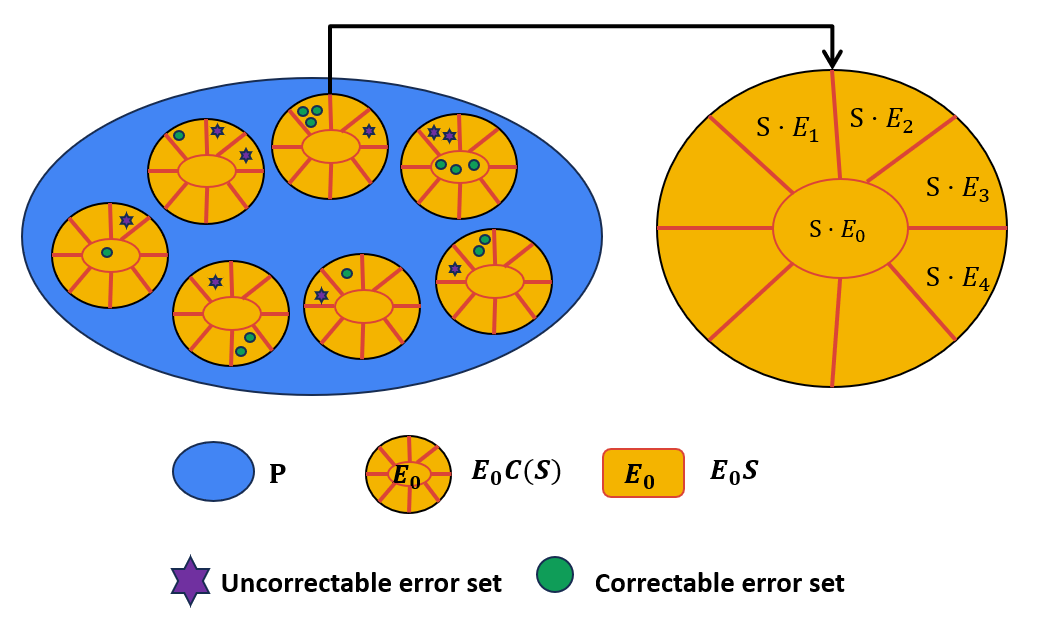
\includegraphics[width=0.8\linewidth]{Figures/stabiQEC.png}
    \caption{This figure show the scheme of stabilizer based error correction. It first divide possible Pauli matrix sets $P$ into subsets $E_0 \mathbf{C}(\mathcal{S})$ inside which all present the same syndrome. Then in each such subset, it splits into sub-subsets $E_i \mathcal{S}$ again, inside which are Pauli matrix that only different with stabilizers. An error set is correctable iff error elements only exsit on single sub-subset for every subsets. We give examples of correctable error and uncorrectable error in this figure     }
    \label{fig:stabilizers_QECC}
\end{figure}
The theorem above gives a correctable criterion for stabilizer QECC. If we further defined \textbf{code distance} as:
\begin{align}
    d = \min_{g\in \mathbf{C}(\mathcal{S}) - \mathcal{S}} |g|,
\end{align}
where $|\cdot|$ counts the non-identity terms in the tensor product of the Pauli matrix. Then any error $E$ satisfied $|E| < d$ could be detected for a non-zero syndrome. Further more, if $\forall~E_i \in \mathbb{E}, |E_i| < \lfloor \frac{d}{2}\rfloor$, then we concludes that $|E_j^\dagger E_i| < |E_j|+|E_i| < d$, thus $E_j^\dagger E_i \notin \mathbf{C}(\mathcal{S}) - \mathcal{S}$ and the error set $\mathbb{E}$ is correctable. In practice, we hope to find a code with large code distance $d > 2t + 1$ to ensure that error sets contain at most $t$-length error are correctable.

We noted that to correct an error channel in practice, ones have to build a map from syndrome to the expect errors. According to the discussion above, ones just corresponds every syndrome(\emph{i.e.}~the subset in Figure~\ref{fig:stabilizers_QECC}) to arbitrary element in the unique sub-subset that contains the channel errors in this subset. In a more realistic error model, all kinds of Pauli errors exist with non-zero probability. Every sub-subset in each subset contains channel errors and thus impossible to implement perfect correction. To solve this problem, we correspond the most probable sub-subset to this syndromes,  which will be further discussed in the next section.

In the end of this section, we generalize the discussion above to continuous errors with an arbitrary form of $E_a$, we first noted that $E_a=Q =\sum_{i = 0}^{4^N - 1} a_i P_i $, where $P_i \in G_N$.
Then we prove the theorem below:
\begin{theorem}\label{theorem:continous_to_Pauli}
    If a stabilizer QECC corrects Pauli errors $P_j$, it also corrects their combination: $Q = \sum_j \alpha_j P_j$. 
\end{theorem}
\begin{proof}
    For any $\ket{c} \in V(\mathcal{S})$ and $\forall~g_i \in \mathcal{S}$, 
    \begin{align}
        g_i Q \ket{c} = \sum_j (-1)^{l_{i,j}} \alpha_j P_j \ket{c}.
    \end{align}
    Noticed that $P_j\ket{c}$ are eigenvectors of operator $g_i$, thus the non-demolition measurement on this operators will generate result $(-1)^{l_{i,j}}$ with post-measurement state $P_j\ket{c}$. This means that during the stabilizer-measurement procedure(The measurement of the first stabilizer $g_i$), error $Q$ will reduced to one of correctable Pauli error, $E_i$, and also, gives the error indicator $l_{i,j}$ corresponding to this Pauli error. Then the proceeding stabilizer QEC procedure will lead to the correct state because $E_i$ is correctable as we supposed.

    Effectively, given a continuous error channel $\Lambda(\rho) = \sum_\mu Q_\mu \rho Q_{\mu}^\dagger$,  we could regard it as a Pauli error channel $\Lambda_e(\rho) = \sum_{\mu,j}|\alpha_j^{(\mu)}|^2 P_j \rho P_j$. We have already used this equation to analysis the effective Pauli error channel of the $\text{CPHASE}$ gates.  
\end{proof}

\paragraph*{Examples: [7,1,3]-Calderbank-Shor-Steane codes---\!\!\!}
A $[n,k,d]$ classical code, denoted as $\mathcal{C}$, is the set of all the length-$n$ string, denoted as $s$, that satisfied $As^T = 0$ for $(n - k)\times n   $ matrix, denoted as $A$, with orthogonal rows. 
These orthogonal rows form another code, which is denoted as $\mathcal{C}^{\perp}$. 
The additional parameter $d$ is the code distance defined by the minimum weight of non-zero $s$, which decides the error correction power of the codes. 
Such a code divides the $2^n$ code space into $r = 2^n / 2^k$ cosets. 
To correct all the $t$-digit error, $r = \sum_{i = 1}^t C_{n}^i$.  
To construct CSS codes, we choose two classical error-correcting codes $\mathcal{C}:[n,k,d]$ and $\mathcal{C}':[n,k',d']$ with parity matrix $A$ and $A'$ and satisfied $\mathcal{C'} \subset \mathcal{C} $. 
We then partition $\mathcal{C}$ into $N = 2^k / 2^{k'}$ cosets of a subset $\mathcal{C}'$ and correspond each coset with quantum code words as below:
\begin{align}
    \ket{\Bar{c}_i} = \frac{1}{\sqrt{2^{ k'}}} \sum_{c' \in \mathcal{C}'} \ket{c_i + c'}, \notag \\
    \text{where,~} \mathcal{C} = \mathcal{C}' \cup (c_1 + \mathcal{C}') \cup \cdots \cup (c_N + \mathcal{C}').
\end{align}
We noted that for $e,f \in c_i + \mathcal{C}'$, $\ket{\Bar{e}} = \ket{\Bar{f}}$ will be satisfied. The identity below should be satisfied:
\begin{align}
    \bigotimes^n_{j=1} H_j \ket{\Bar{c}_i} &= \frac{1}{\sqrt{2^{n+ k'}}} \sum_{c' \in \mathcal{C}'} \sum_{w \in \mathbb{F}_2^n}(-1)^{w \cdot (c_i + c')^T } \ket{w} \notag \\
    &= \frac{1}{\sqrt{2^{n+ k'}}}  \sum_{w \in \mathbb{F}_2^n} (-1)^{w \cdot c_i^T} \left[\sum_{c' \in \mathcal{C}'} (-1)^{w \cdot c'^T }\right] \ket{w} \notag \\
    &= \frac{1}{\sqrt{2^{n+ k'}}}  \sum_{w \in \mathcal{C}^{'\perp}} (-1)^{w \cdot c_i}  \ket{w}.
\end{align}
This is a vector in space spanned by strings in $\mathcal{C}^{'\perp}$. One then could choose classical codes $\mathcal{C},\mathcal{C}^{'\perp}$ that correct all the $t$-digit errors. This will lead to QEC codes that correct all the $t$ bit-flip and $t$ phase-flip errors. To detect the error without destroying encoded information, we first noted that $\ket{\Bar{c}_i} \in V(\mathcal{C})$ and $\bigotimes^n_{j=1} H_j \ket{\Bar{c}_i} \in V(\mathcal{C}'^\perp)$ are equivalent to:
\begin{align}
    \prod_{i = 1}^n X_i^{A_{ji}} \ket{c} = \ket{c}, ~\forall~j = 1, \cdots, n-k , \\
    \prod_{i = 1}^n Z_i^{A_{ji}^{'\perp}} \ket{c} = \ket{c}, ~\forall~j = 1,\cdots,k'.
\end{align}
These $n - (k - k')$ numbers of stabilizers restrained the code space into a $2^{k - k'}$ dimensional space. Then we could use non-demolition measurements to measure stabilizers. Their results will identify all the $t$-qubits errors. 

When $t = 1$, we choose $\mathcal{C} = CSS[7,4]$ and $\mathcal{C}' = CSS~[7,3]$. It turns out that $\mathcal{C} = \mathcal{C}^{'\perp}$ and
\begin{align}
    A = \begin{pmatrix}
        1&0&0&1&1&1&0 \\
        0&1&0&0&1&1&1 \\
        0&0&1&1&1&0&1
    \end{pmatrix} =A^{'\perp}.
\end{align}
\paragraph*{Examples: Surface codes and Toric codes---\!\!\!}
The first Surface codes is Kitaev's toric code~\cite{kitaev2003fault}. Qubits are placed on the edge of toric edges such that satisfied the periodic boundary conditions. Its stabilizers then constitute all the $Z$ operators on plaquette and $X$ operators on stars. It is obvious that those star operators and plaquette operators commute with each others. Noticing that the numbers of independent stabilizers is $2L^2 - 2$ (The product of all plaquette-$Z$s and star-$X$s are identity), this code use $2L^2$ qubits to encode two logical qubits. Interestingly, the elements in $C(\mathcal{S}) - \mathcal{S}$ constitute a circle on the toric surface that cannot shrink into a point, which is topologically different compared to trivial errors in $\mathcal{S}$. 
\begin{figure}[!hbtp]
    \centering
     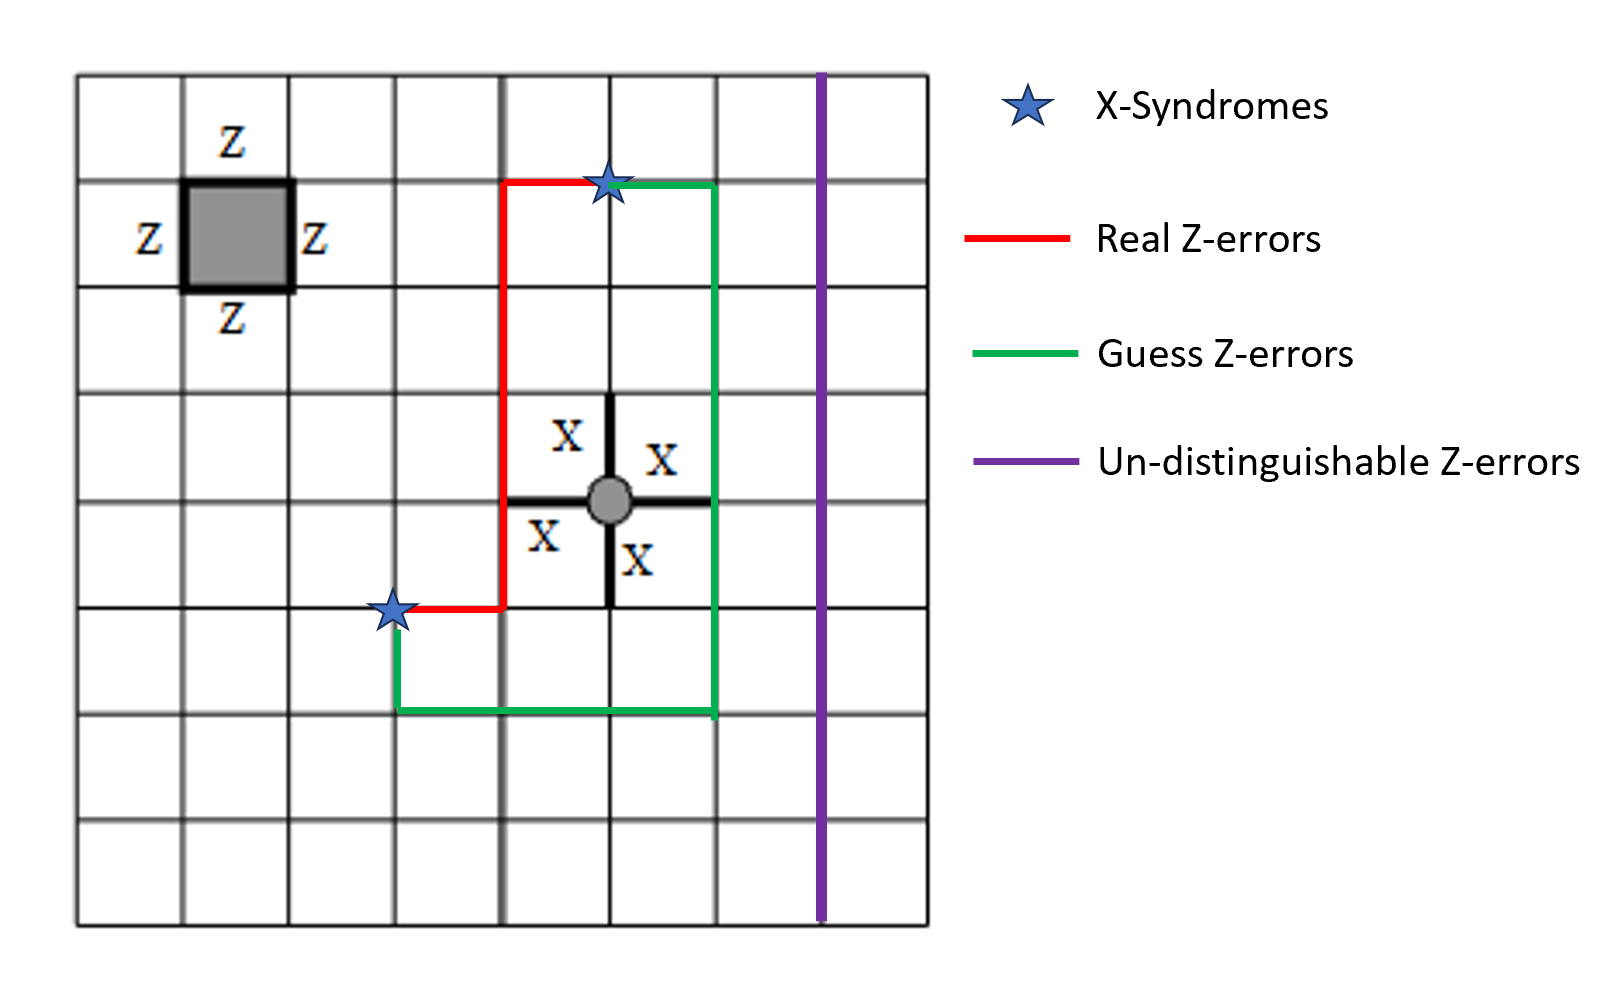
\includegraphics[width=0.45\linewidth]{Figures/surfacecode0.png}
    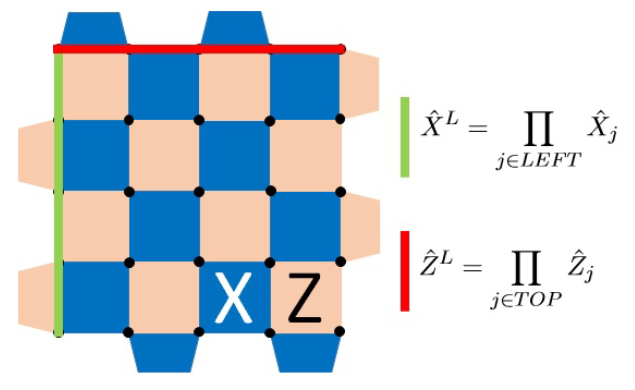
\includegraphics[width=0.45\linewidth]{Figures/rotated_surface_code.png}
    \caption{Stabilizers of toric code (left). A patch of rotated surface code with code distance d = 5 (right).}
    \label{fig:surfacecode}
\end{figure}
Certain Pauli $Z$ errors appeared on this code could be represented by a set of edges. The star-$X$ stabilizers will show syndromes at the boundary of those edges(every ends of the edges). To guess the possible $Z$ errors from those syndromes, ones has to select on connection method of those ends. If the selected connection method is on a different topological class of the real connection error that corresponds to the real $Z$ errors, the surface code will make a false.

\subsection{Decoders for surface codes}
In the discussion of the previous section, we try to perfectly correct an error channel. This target is too strong such that we have to make sure certain equivalent Pauli errors will not contained in the error channel. In the real world, error channel contained every equivalent Pauli channel, but with different error rates. This means that logical qubit still suffer with certain logical Pauli error $X_L,Y_L,Z_L$ with certain logical error rate $p_{Lx},p_{Ly},p_{Lz}$. 

In this section, we focus on the surface code and illustrate different method to implement surface code decoding. We analysis the decoder with plausible error channel is \textbf{independent error channel }that assert each qubits make storage faults independently, with some given error rate $p_x, p_y,p_z$ of $X,Y,Z$ Pauli channel. 

\paragraph{Maximum likelihood decoder}
For surface code, we have aware that the error are divided into two classes, as illustrated in Figure~\ref{fig:surface-equivalence}.  Though ones cannot expect only the error in single class will exist, we could calculate the probability that one error located in each one of them and correspond this syndrome to the class that most likely to happen. We called this strategy as \textbf{Maximum likelihood decoding}. 
\begin{figure}
    \centering
    \begin{minipage}[t]{0.45\textwidth}
           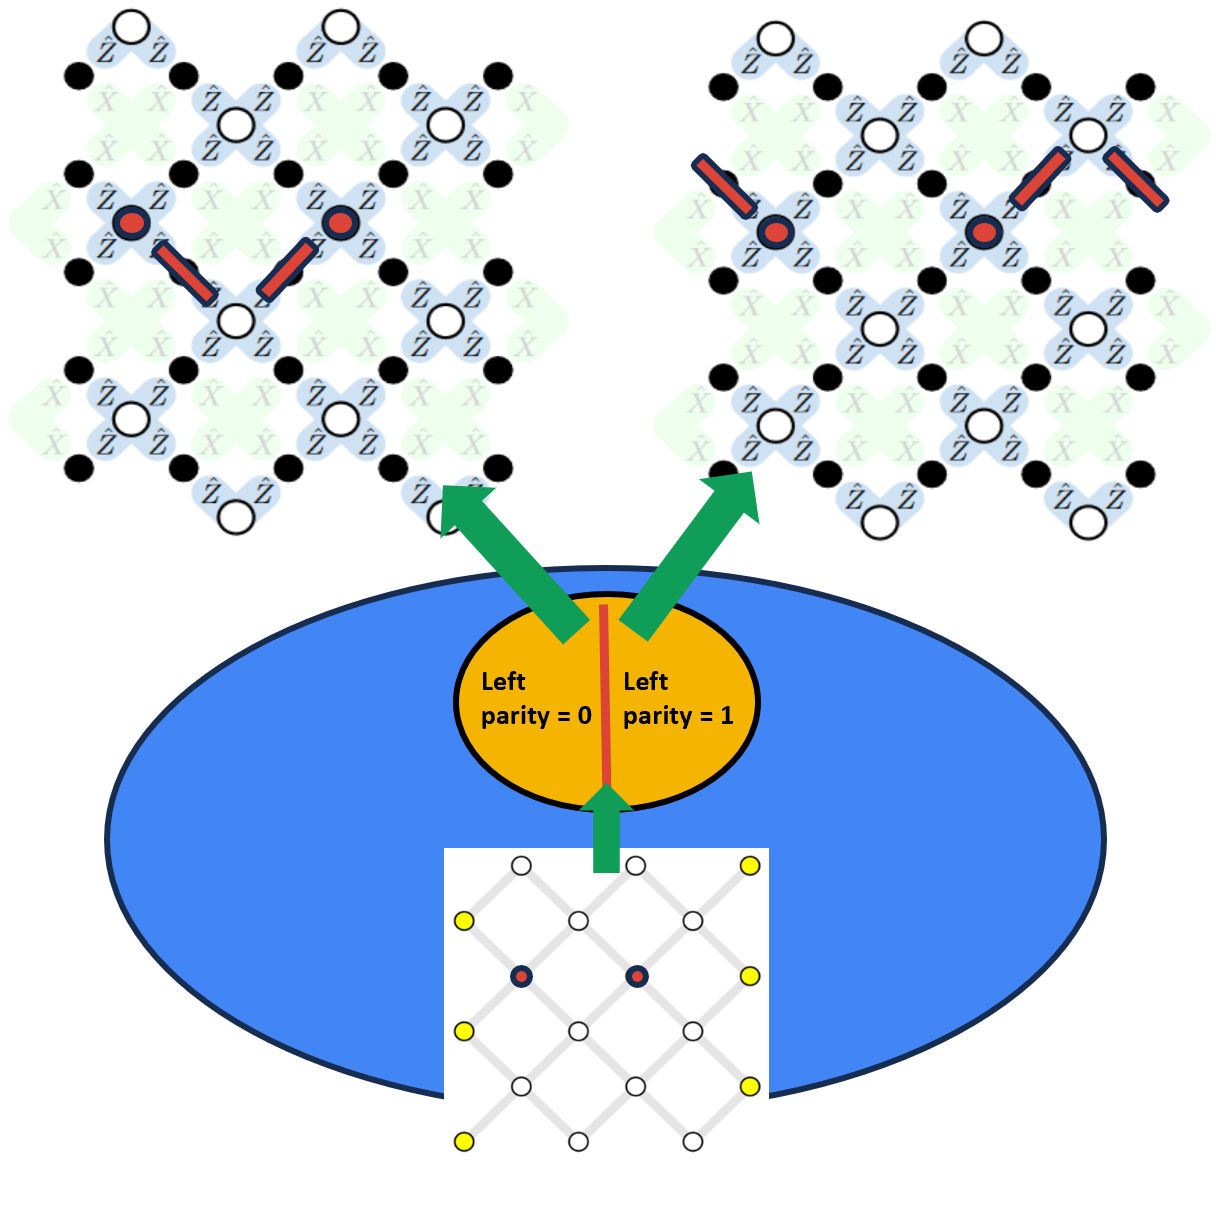
\includegraphics[width=0.8\linewidth]{Figures/equivalence_class_surfacecode.png}
             \caption{The yellow set is the error that gives the same $\text{Z-}$syndrome. This set is divided into two classes under quotient of stabilizers. considering the shape of $\text{Z}$ stabilizers, we represent $\text{X-}$syndrome as edges that connect syndromes. Edges ended on syndrome or lattice boundary are those error that present this syndrome. We count the number of edges that ended at left(or right) edge. The parity of this number manifest which equivalence class it belongs to.}
                \label{fig:surface-equivalence}
    \end{minipage}
       \hspace{0.07\textwidth}
 \begin{minipage}[t]{0.45\textwidth}
        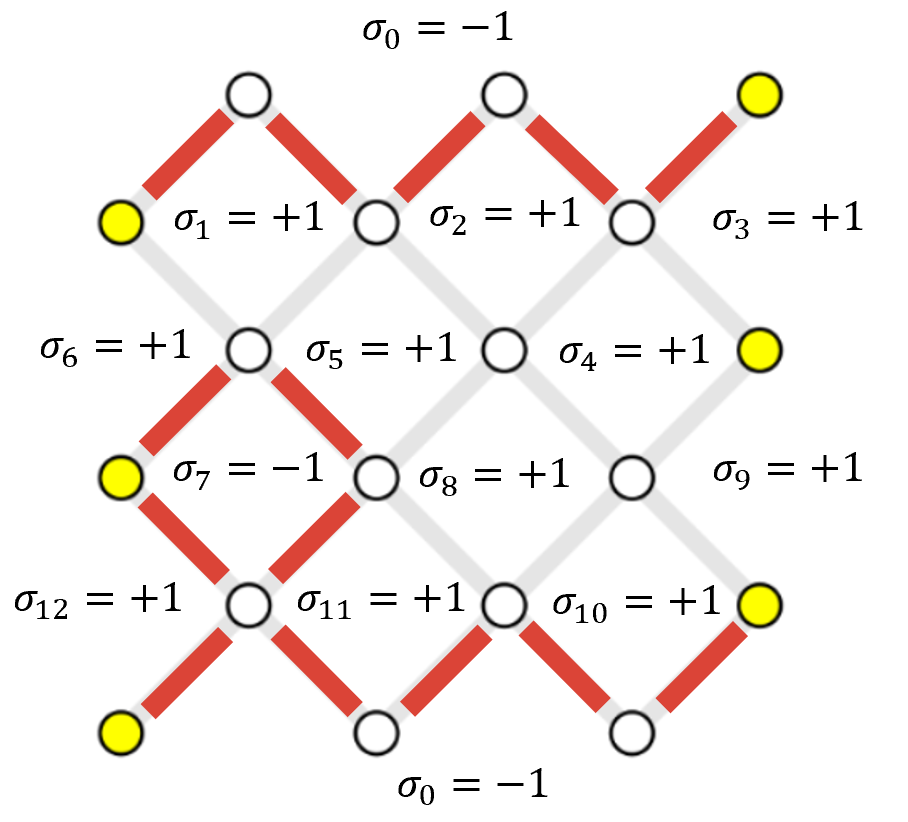
\includegraphics[width=0.8\linewidth]{Figures/syndrometospin.png}
        \caption{The effective spin on the lattice. We designate $\{+1,-1\}$ to each $\sigma_i$. $u_l = -1$ if $\sigma_i$ and $\sigma_j$ are different and $u_l = 1$ if they are the same. Then this designation corresponds to edges that are one of the $\text{X}$ stabilizers and $u_l = \sigma_i \sigma_j$. With this observation, we can transform the summation over edges to summation of spin states.}
                  \label{fig:surface_to_spin}
 \end{minipage}
 
  
  
\end{figure}

To adjust the capability of surface code with length $L$ to correcting certain error model using maximum likelihood decoding, we adopt the $\text{XZ-}$uniform independent error channel with probability $p$ and calculate the value $\text{Pr}(\bar E)$ that denotes the probability in class that contained $X$-errors $E$. For arbitrary $E$, we have:
\begin{align}
    \text{Pr}({E}) &= \prod_l (1 - p)^{1 - n(l,E)} p^{n(l,E)} = (1 - p)^{N}\prod_l  (\frac{p}{1 - p})^{n(l,E)} \notag \\
    &=(1 - p)^{N} (\frac{p}{1 - p})^{N/2}\prod_l   (\frac{p}{1 - p})^{n(l,E) - 1/2}\\
    &=(1 - p)^{N/2} p^{N/2}\prod_l  \text{exp}\left[{\frac{1}{2}\ln (\frac{1-p}{p}) u(l,E)}\right] \\
    &=A(p)\prod_l  \text{exp}\left[{J u(l,E)}\right],
\end{align}
where $u= 1 -2n$ and $u(l,E) = -1$ if $l \in E$ , $u(l,E) = 1$ otherwise. $J = \frac{1}{2}\ln (\frac{1-p}{p})$ Then we find that:
\begin{align}
    \text{Pr}(E +E') = A(p)\prod_l  \text{exp}\left[{J u(l,E)u(l,E')}\right]
\end{align}
Then we have:
\begin{align}
    \text{Pr}(\bar E) &=  \sum_{C \in C_{\mathcal{S}}} \text{Pr}(E + C) \\
    & = \sum_{C \in C_{\mathcal{S}}} A(p)\prod_l  \text{exp}\left[{J u(l,E)u(l,C)}\right]\\
    &=\frac{1}{2}A(p)\sum_{\sigma \in \{-1,1\}^N}\prod_{\langle i,j\rangle}  \text{exp}\left[{J u(l_{ij},E) \sigma_i \sigma_j}\right]
\end{align}
Such a summation is equivalent to partition function $Z_E$ for certain classical spin models with quench or frustration ~\cite{Chubb_2021}.
\begin{align}
   \text{Pr}(\bar{E}) =\frac{1}{2}A(p)\sum_{s} e^{J\sum_{i j} \eta_{ij}(E) s_i s_j} =: \frac{1}{2}A(p)Z_E
   \label{eq:equi_proba_to_partition}
\end{align}
Here spins are on each $\text{X}$ stabilizers. $\eta_{ij} = -1$ if the junction edge of stabilizer $i$ and stabilizer $j$ are in error set $E$ and $\eta_{ij} = 1$ otherwise. This equation manifest that the task to find equivalent class probability of $E$ is the same as calculate the partition function of a frustrated spin model with frustration on error position. 

If $\text{Pr}(\bar{E}) > \text{Pr}(\overline{E + D})$, for $D$ as a non-trivial $\text{X}$-circle depicted in Figure~\ref{fig:surfacecode}, we correct the syndrome with $\text{X-}$string in $\bar E$.  The correctness of this correction is bench-marked by the information entropy:
\begin{align}
    \mathcal{E}(S) = -\frac{\text{Pr}(\bar E_s)}{\text{Pr}(S)} \ln \frac{\text{Pr}(\bar E_s)}{\text{Pr}(S)}  - \frac{\text{Pr}(\overline{E_s + D})}{\text{Pr}(S)} \ln \frac{\text{Pr}(\overline{E_s + D})}{\text{Pr}(S)} ,
\end{align}
where $S$ is the syndrome the $E_s$ is anyone of the error that present such syndrome. When dealing with syndrome $S$, the smaller the $\mathcal{E}(S)$ is, the probability will more concentrate to one of the equivalence class thus give a lower probability to make faults. 
 Considering all the syndrome, the average information entropy writes:
\begin{align}
    \bar{\mathcal{E}} = \sum_S \text{Pr}(S) \mathcal{E}(S) &=-\frac{1}{|\bar E|}\sum_E \text{Pr}(\bar E) \ln \frac{\text{Pr}(\bar E)}{\text{Pr}(S_E)} ,\\
    &=-\sum_E \text{Pr}(E) \ln \frac{\text{Pr}(\bar E)}{\text{Pr}(S_E)} \\
    &= \sum_E \text{Pr}(E) \ln \left(1 + \frac{\text{Pr}(\overline{E+D})}{\text{Pr}(\bar E)}\right)
\end{align}
where $|\bar E|$ is the number of error that equivalent to $E$, which evaluates as $N - 1$ where $N$ is the number of the effective spin. The condition that $\lim_{L \to \infty}\bar{\mathcal{E}} =0$ now became 
\begin{align}
  \lim_{L \to \infty} \sum_E \text{Pr}(E) \ln Z_{E}  - \sum_E \text{Pr}(E+D) \ln Z_{E}  = +\infty 
\end{align}
Through defining free energy for the \textbf{Random Bonded Ising Model(RBIM)} as: $F_E = - \ln Z_E$, we concludes that finding the threshold is equivlent to find the condition that RBIM has energy gap between two topological phase. 
The phase transition of RBIM has been further discussed in previous research, which gives us the accuracy threshold using maximum likelihood decoder with $p_{th} \approx 0.11$~\cite{Dennis_2002}. 

\paragraph{Minimum weight perfect matching---\!\!\!}
The maximum likelihood decoders, although applicable to arbitrary stabilizer codes, have been proven to be NP-complete \cite{PhysRevA.83.052331}. However, focusing on Equation (1) as $ p \to 0 $, $ J \to +\infty $, and the minimized $ H = -\sum_{i j} \eta_{ij}(E) s_i s_j $ predominantly takes effect. Given syndromes corresponding to two error-induced frustrations $ E $ and $ E + D $, we can identify ground states with respect to these frustrations and select the one with lower energy. This process effectively involves finding the minimum weight perfect matching of the given syndromes, achievable through the Minimum Weight Perfect Matching (MWPM) decoder utilizing Edmond’s blossom algorithm.

A weighted graph is defined as $ G = (V=\{v_i\},E = \{(v_i,v_j), \forall i \neq j\},W= \{w_e \in \mathbb{R}, \forall e \in E\}) $. A matching of $ G $ is a subset $ M $ of edges $ E $ such that elements of $ M $ share no vertices. A perfect matching of $ G $ is a matching such that every vertex is contained in an edge. Here, we focus on a graph with a boundary, denoted as a special vertex $ v_0 $. A perfect matching of a graph with a boundary is a subset $ M $ of $ E $ such that every vertex in $ V $ except $ v_0 $ is contained in one element of $ M $, and any two elements in $ M $ have no shared vertex unless the shared vertex is the boundary $ v_0 $.

For $ e \in E $, $ x_e = 1 $ if $ e \in M $ and $ x_e = 0 $ otherwise. The minimization task becomes:

\begin{align*}
    &\text{minimize} \sum_{e \in E} w_e x_e \\
    &\text{subject to} \sum_{e \in \delta(\{v_i\})} x_e = 1, \forall i = 1,2,\cdots,|V|-1 \\
    &\quad \quad \quad \quad \quad x_e \in \{0,1\}
\end{align*}

This optimization involves a convex function on a finite set $ \mathcal{F} $. Discreteness can be eliminated by optimizing on the convex hull of $ \mathcal{F} $, transforming it into a traditional convex optimization task:

\begin{align}
    &\text{minimize} \sum_{e \in E} w_e x_e \\
    &\text{subject to} \sum_{e \in \delta(\{v\})} x_e = 1, \forall v \in V - \{v_0\} \\
    &\quad \quad \quad \quad  \sum_{e \in \delta(\mathcal{O})} x_e \geq 1, \forall O \in \{S \subset V - \{v_0\} |~|S| ~\text{is odd and  >1}\} \\
    &\quad \quad \quad \quad  x_e \geq 0,~\forall e \in E
\end{align}
which gives a efficient solution with time complexity $\mathcal{O}(|V|^{2.5})$~\cite{wu2023fusion}, where $V$ is the set of syndromes 

We first clearify the definition of a decoding graph and a syndrome graph, as depict in Fig~\ref{fig:decoding_graphs}
\begin{figure}
    \centering
    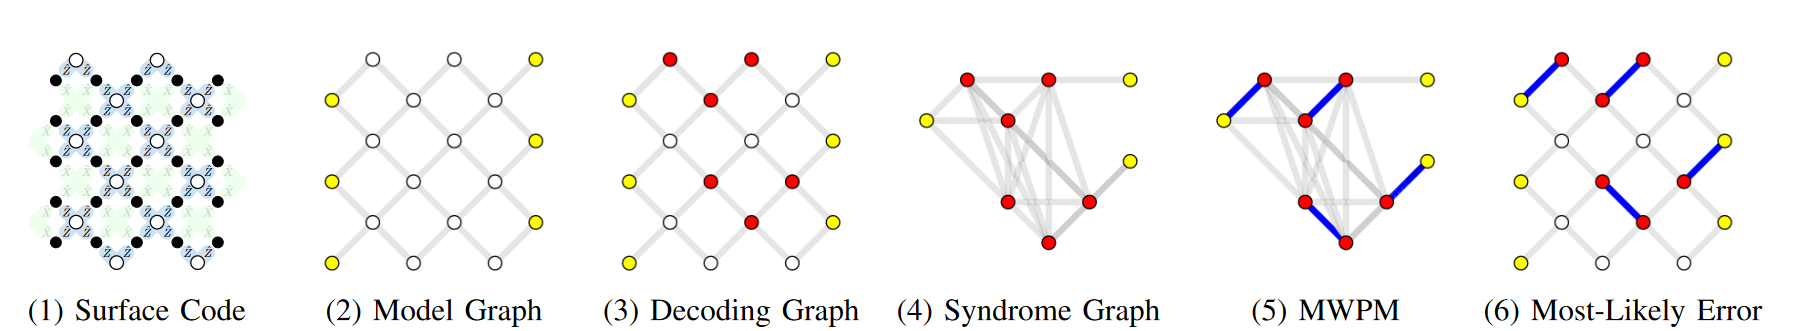
\includegraphics[width=0.9\linewidth]{Figures/syndrome_graph.png}
    \caption{Different graphs during the decoding procedures~\cite{wu2023fusion}}
    \label{fig:decoding_graphs}
\end{figure}

\paragraph{Union Find decoder}
To deal with erasure errors, a efficient decoder is designed~\cite{Delfosse_2020}. In the process of predicting errors in a surface code quantum system, where syndromes occur at incorrect boundaries and are characterized by the Syndrome set $\sigma$ and the erasure error set $\mathcal{E}$, a method is employed to generate errors with complexity linearly dependent on the number of bits.
\begin{figure}
    \centering
    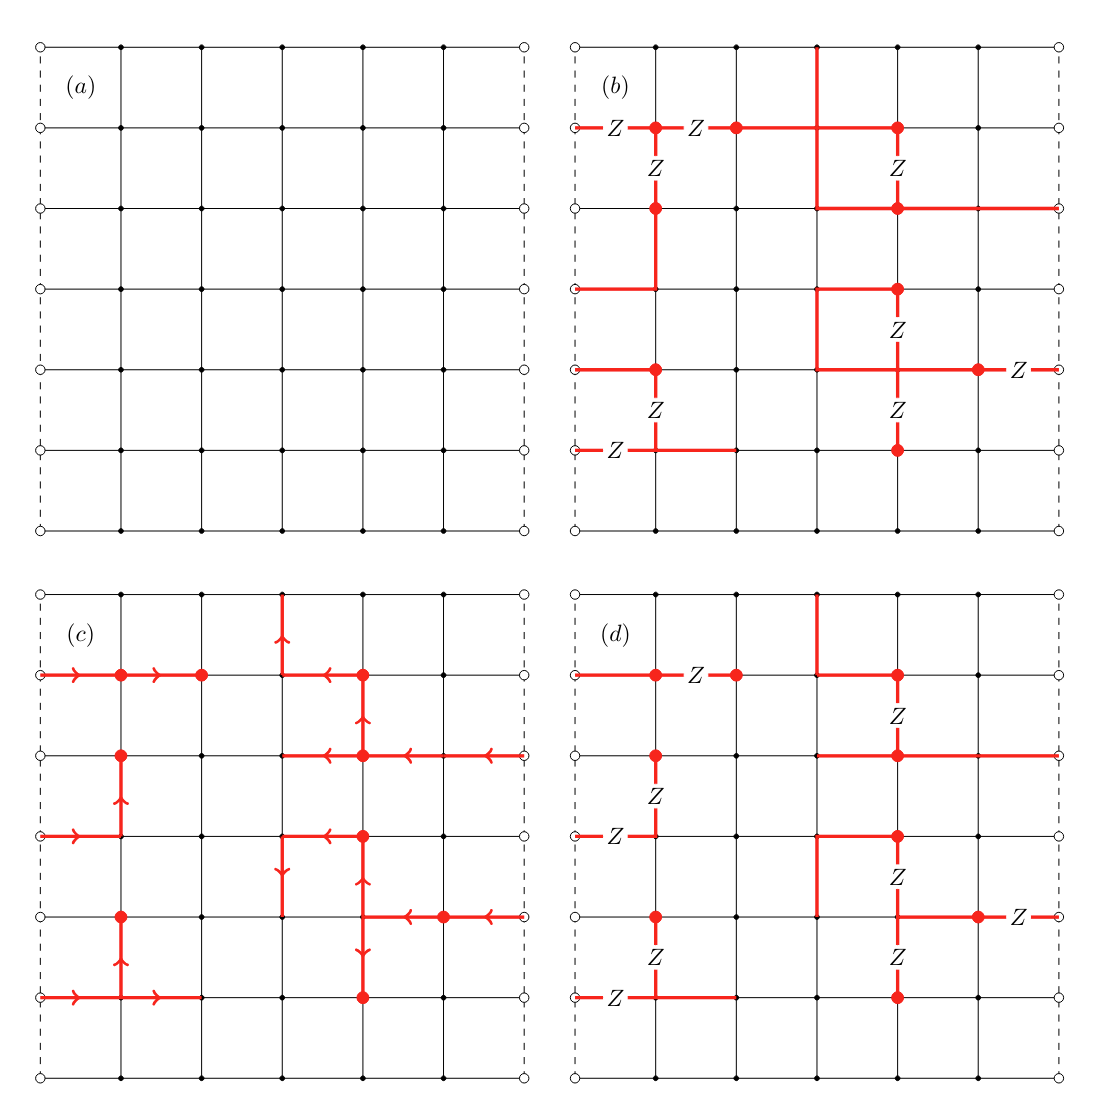
\includegraphics[width=0.5\linewidth]{Figures/union_find.png}
    \caption{In the case of a boundary-enriched surface code, syndromes (depicted as red dots) and erasure errors (illustrated by red lines) are observed. The actual and predicted errors are marked with 'Z'.}
    \label{fig:union_find}
\end{figure}

As showed in Figure~\ref{fig:union_find}, initially, a tree graph is constructed from the erasure error set $\mathcal{E}$ by starting with a seed vertex and gradually adding edges.
Subsequently, starting from the leaves of this tree, edges are sequentially removed.
If a removed leaf has a syndrome at its unconnected end, it is added to set $A$, and the other end is reversed to maintain balance between having and not having a syndrome. 
Once all leaves are removed, the resulting set A represents the predicted errors. 
In cases of surface codes with boundaries, the selection of seed points lacking certain measurements on the boundary facilitates the generation process.

\subsection{Syndrome extraction in surface codes}

\subsubsection{Syndrome extraction circuit}
\paragraph*{Non-demolition measurement and Hadamard test---\!\!\!}
The realization of the surface codes require the extraction of the measurement result of stabilizers $\{g_i\}$ while keep states in the code space. This calls for non-demolition measurement, which in general could be expressed as Hadamard test of certain quantum states. 
\begin{figure}[!hbtp]
\centering
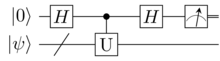
\includegraphics[width=0.4\linewidth]{Figures/Hadamard_test_measure_real.png}
    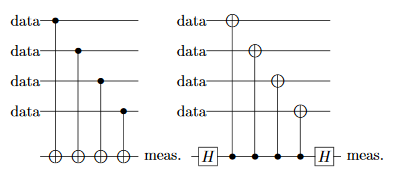
\includegraphics[width=0.4\linewidth]{Figures/XXXX_ZZZZ_meas_circuit.png}
   \caption{The Hadarmard test circuit(Left) and the syndrome extraction circuit for surface codes(Right). \cite{Dennis_2002}}
\label{fig:Hadarmard_test}
\end{figure}
\begin{theorem}
    The Hadamard test runs quantum circuit as showed in Figure~\ref{fig:Hadarmard_test}. The first qubit is measured on $\{\ket{0},\ket{1}\}$ basis. The measurement result turns out to be $0,1$ with probability:
\begin{align}
    p(0) = \text{tr}(\rho \frac{2\mathbb{I} + U + U^{\dagger}}{4}), \\
      p(1) = \text{tr}(\rho \frac{2\mathbb{I} - U - U^{\dagger}}{4}) ,
\end{align}
and post measurement state:
\begin{align}
    \{\ket{0}\!\bra{0} \otimes \frac{\mathbb{I} + U}{2} \rho \frac{\mathbb{I} + U^{\dagger}}{2},\ket{1}\!\bra{1} \otimes \frac{\mathbb{I} - U}{2} \rho \frac{\mathbb{I} - U^{\dagger}}{2} \}
\end{align}
\end{theorem}
When $U$ is Pauli operator $g_i$, its Hadarmard test turns out to be non-demolition measurement of $g_i$. Using this theorem, we construct the circuit below to implement syndrome extraction of $\text{XXXX}$ stabilizers and $\text{ZZZZ}$ stabilizers.

\paragraph*{Parallel syndrome extraction---\!\!\!}
 The distribution of the error is highly related to the syndrome extraction circuit order. Here we first show that the $\text{XXXX}$ and $\text{ZZZZ}$ syndrome extraction circuit could be run simultaneously such that the control-$\text{Z}$ gates are all implemented in "North-West-East-South" order. The proof of this is sketched in Figure~\ref{fig:z-shape_order}.
\begin{figure}[!htbp]
    \centering
    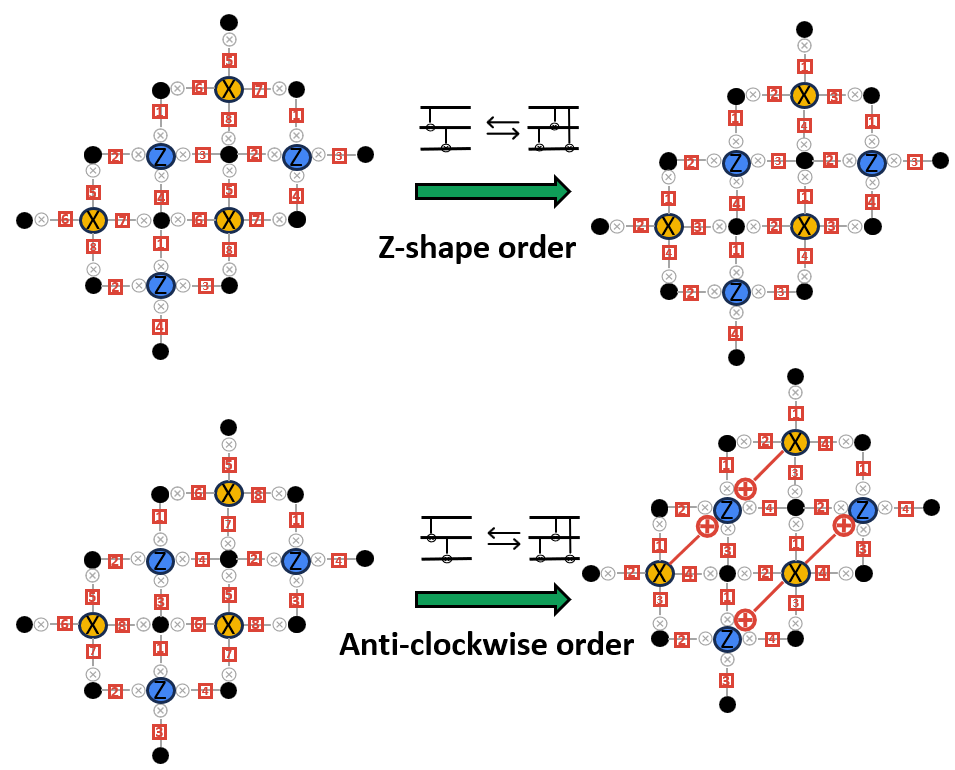
\includegraphics[width=0.7\linewidth]{Figures/z-shape_order.png}
    \caption{Enter Caption}
    \label{fig:z-shape_order}
\end{figure}
In the left-side of the figure, we plot the circuit that implement $\text{ZZZZ}$ measurements first and then the $\text{XXXX}$ measurements. To change to the Z-shape simultaneous order or the anti-clockwise simultaneous order, we have the move certain non-commutative $\text{CNOT}$ gates, which introduces multiple $\text{CNOT}$ gates with control qubits $\text{X-}$ ancilla qubits and control qubits $\text{Z-}$ ancilla qubits, as ploted in the right hand side. This explain why we should adopt Z-shape simultaneous order. 

\subsubsection{QECC with circuit error}

We noted that in Figure~\ref{fig:Hadarmard_test}, the ancilla qubits exists storage error. The $\text{CNOT}$ gates also has biased error as showed in the control-Z gate simulation. To be specific, during the ancilla qubit preparation procedure, we supposed that we has $p_p$ probability to prepare an opposite states and probability $p_m$ to get a opposite ancilla qubit measurement result. (We do not need to consider the continuous error for theorem~\ref{theorem:continous_to_Pauli}). The faulty $\text{CNOT}$ gate is described by one perfect $\text{CNOT}$ gate followed by Pauli gates $\sigma_i \otimes \sigma_{j}$  with probability $p_{ij}$.

With this consideration, the syndrome extraction circuit is poorly designed so that a sole preparation mistake in the ancilla or $\text{CNOT}$ gates error may spread to multiple qubits within the code block, thereby representing an equivalent \textbf{storage error} on data qubits and \textbf{syndrome extraction error} that correlated to each others. 

In this section we discuss how to deal with such a circuit based error and briefly show how storage error and syndrome extraction error related.
 

\paragraph*{Syndrome extraction error---\!\!\!}
To deal with the syndrome measurement error, instead of correct qubits based on only single measurement result, ones implement the syndrome extraction circuit $M $ times and find error based on syndromes on these $M$ times measurement result. Intuitively, $M = d$  if the syndrome measurement error is comparable to storage error.

To be specific, we consider that Alice hope to protect a given logic $\ket{0}_L$ state from storage error and syndrome measurement error within time $T$ and then measured local $\text{X}$ operators on all data qubits. At the first implementation of the syndrome extraction circuit in Figure~\ref{fig:Hadarmard_test}, he denotes the ancilla qubits with $-1$ result as syndrome. In the following $M - 1$ times measurements, he attached syndromes on ancilla qubits if their measurements value changed compared to the last turn.
\begin{figure}[!hbtp]
    \centering
    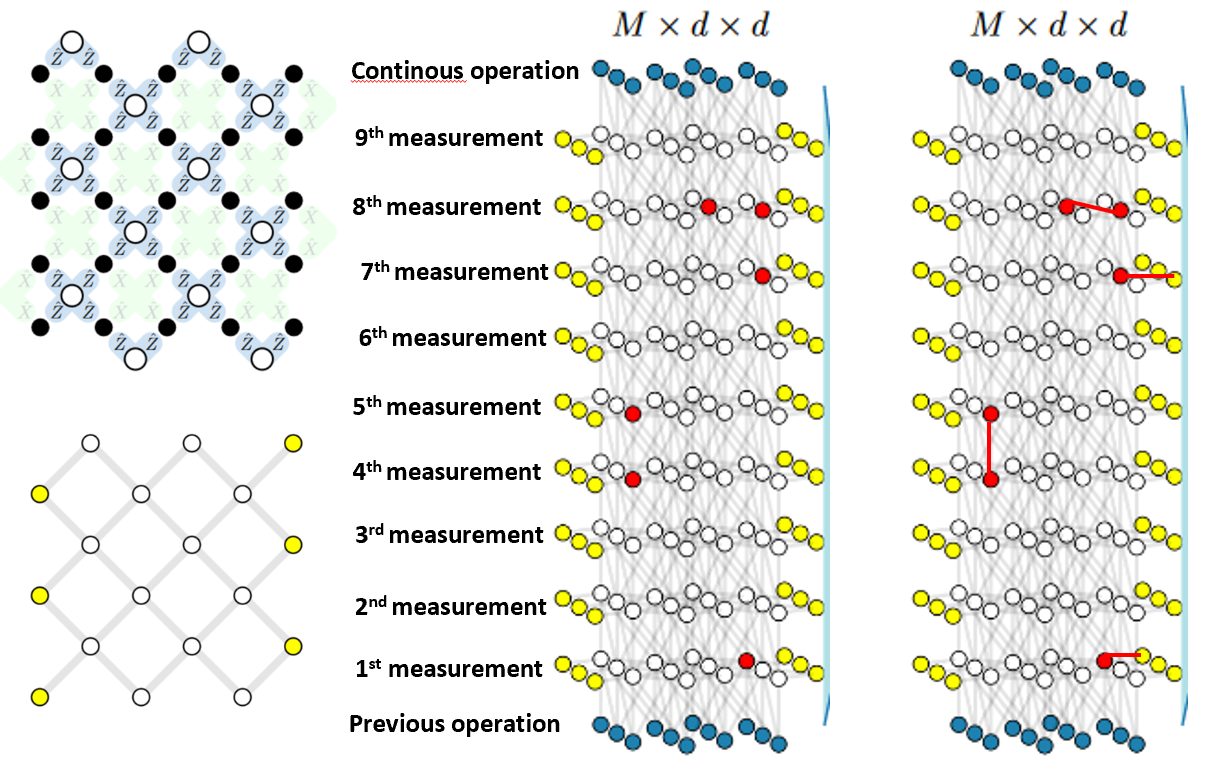
\includegraphics[width=0.9\linewidth]{Figures/multird_qec.png}
    \caption{The syndrome and decoding process in a multi-round surface codes. This mitigates the effect of syndrome extraction error.}
    \label{fig:multird_qec}
\end{figure}


Similar to the one-round surface code, the edge in the space means a qubit flip. A time-like edge means one syndrome extraction error happens before these two syndromes. Given a set of edges in spacetime, Alice could implement all the space-like edges to repair the errors. Any set of edges that perfect match the syndromes constitute an error pattern that raise such syndromes. 
Perfect matching path $A,B$ are equivalent if the repair of $A$ could repair the error $B$ either. Then given certain syndromes, their perfect matching paths could be devided into two classes through counting the number of syndromes that connect with left yellow surface and right yellow surface. 

Noted that in Figure~\ref{fig:multird_qec}, the measurement results of all local $\text{X}$ operators of data qubits is represented on the "Continuous operation"  tag. The $\text{XXXX}$ syndromes could be referred from the measurement results, which we believed that no syndrome extract error exists.  For the syndrome extraction error during the fault-tolerant computation process, the last measurement of the $M\text{-th}$  syndrome measurements could be faulty, which will be deal with more carefully in the next section.

\paragraph*{Error propagation analysis---\!\!\!}
To find the equivalent storage error on data qubits and syndrome extraction error, we move all the error on data qubit to the beginning of each syndrome extraction circuit. This corresponds to certain storage error that happened before this round measurement. The Pauli error at ancilla qubits could be move to the end and replaced by a syndrome extraction error at this round. This means that we can regard the preparation, measurement and gates all perfect, at a cost of introducing correlated Pauli error and measurement error, as illustrated in Figure~\ref{fig:error-propagation}
\begin{figure}[!htbp]
\centering
\begin{minipage}[t]{0.48\textwidth}
\begin{quantikz}[row sep=0.3cm, column sep=0.3cm]
    \lstick{$\ket{0}$}        & \qw & \gate{H} & \ctrl{1} &\gate{X}&\ctrl{2} & \ctrl{3} & \ctrl{4}   &\gate{H} & \meter{} \\
    \lstick{N} & \qw  & \qw      &\targ{}  &\gate{Z}& \qw      & \qw     & \qw         & \qw     & \qw\\
      \lstick{W} & \qw & \qw      & \qw     &\qw & \targ{}  & \qw     & \qw        & \qw     & \qw\\
        \lstick{E} &\qw& \qw      & \qw      &\qw & \qw      & \targ{} & \qw         & \qw     & \qw \\
         \lstick{S} &\qw& \qw      & \qw     &\qw  & \qw      & \qw     & \targ{}         & \qw     & \qw 
\end{quantikz}
\end{minipage}
\begin{minipage}[t]{0.48\textwidth}
\begin{quantikz}[row sep=0.3cm, column sep=0.3cm]
    \lstick{$\ket{0}$}        & \qw & \qw& \gate{H} & \ctrl{1}     &\ctrl{2} & \ctrl{3} & \ctrl{4}   &\gate{H} & \meter{}&\gate{flip} \\
    \lstick{N} & \qw  & \gate{Z}& \qw      &\targ{}  & \qw      & \qw     & \qw         & \qw     & \qw & \qw\\
      \lstick{W} & \qw & \gate{X}& \qw       & \qw      & \targ{}  & \qw     & \qw        & \qw     & \qw & \qw\\
        \lstick{E} &\qw& \gate{X} & \qw     & \qw       & \qw      & \targ{} & \qw         & \qw     & \qw  & \qw\\
         \lstick{S} &\qw& \gate{X}& \qw      & \qw       & \qw      & \qw     & \targ{}         & \qw     & \qw  & \qw
\end{quantikz}
\end{minipage}
\caption{This figure show how we compact the distributed error(the left circuit) and equivalent them to correlated storage error before measurement and syndrome extraction flip error(the right circuit)}
\label{fig:error-propagation}
\end{figure}
We show how error propagate in Appendix~\ref{app:error_propagation} . According to the analysis, we conclude that there are mainly two types of error that appeared, which we named the \textbf{hook errors } where one syndrome extraction error and one storage error happens simultaneously and \textbf{claw errors} where two measurement error and one storage error happens simultaneously. 
\begin{figure}[!htbp]
    \centering
    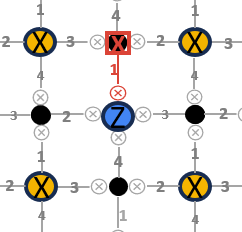
\includegraphics[width=0.2\linewidth]{Figures/hook_error1.png}
    \hspace{0.1\textwidth}
     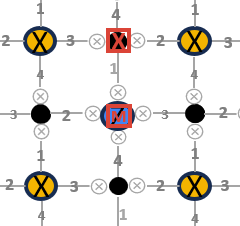
\includegraphics[width=0.2\linewidth]{Figures/hook_error2.png}
    \caption{One $\text{X-}$type error on data qubit after the first $\text{CNOT}$ gate (left) could generate a pair of syndrome extraction error and $X$ storage error. We call this hook error}
    \label{fig:hook-error}
\end{figure}
\begin{figure}[!htbp]
    \centering
    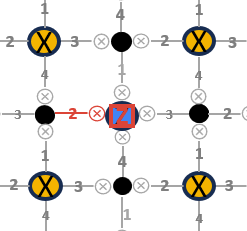
\includegraphics[width=0.2\linewidth]{Figures/claw_error1.png}
    \hspace{0.1\textwidth}
     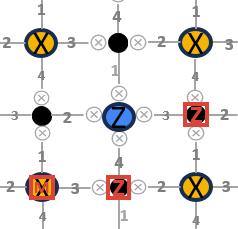
\includegraphics[width=0.2\linewidth]{Figures/claw_error2.png}
    \caption{One $\text{Z-}$type error on ancilla qubit after the second $\text{CNOT}$ gate (left) could generate a triple of error with one syndrome extraction error and two $Z$ storage error. We call this claw error}
    \label{fig:hook-error2}
\end{figure}

To mitigate the correlation-error-effect due to SPAM error, Shor and Steane already have introduced two distinct approaches aimed at curtailing the transmission of errors from ancilla to data during the measurement of the check operators of a stabilizer code.

\section{Fault-tolerant quantum computation}

It is worth noting that error correction codes are only able to correct specific errors. Due to the independent error model, the error rate that two qubits fault simultaneously will be proportional to $p^2$, which is smaller than the single-qubit error rate $p$. Thus codes that could correct all the single-qubit errors will reduce the noise. Nevertheless, this property will not be satisfied if we take the gates errors and storage errors during the encoding, decoding, error detection, and error recovery procedures. For example, if a single-qubit error happens with rate $p$, it will cause a multi-qubit fault in the final result with an identical probability rate. One way to prevent error propagation is through \textbf{fault-tolerant operations} as defined below.
\begin{definition}
    Supposed state information is encoded into logic qubit, which is composed by qubits block and certain QECC $\mathcal{S}$. An operation is said to be fault-tolerant if the occurrence of a single gate error and single qubits error during the operations will cause no more than one qubit error in each block.  
\end{definition}
Transversal gates is defined as one-qubit gates in the code block and two-qubit gates between corresponding qubits in two blocks.  It could be proved that transversal gates are fault-tolerant operations. In the following, we explicitly introduce how to construct transversal gates and implement fault-tolerant operations in different codes.

\paragraph*{Magic state injection---\!\!\!}
In the previous research by Zhou \emph{et.al.}~\cite{PhysRevA.62.052316}, they proposed the one-bit teleportation method based on the ordinary quantum state teleportation. As illustrated in Figure~\ref{fig:onebit_tele}, ones could implement gate $G_b VG_a$ to arbitrary state $\ket{\psi}$ through preparation the state $V H^{\otimes n} \ket{0}^{\otimes n}$ and possible correction $G_b VX^{\otimes n}V^\dagger G_b^\dagger$ on the states. Here $V \in \mathcal{Cl}_3$ is commutative with the control ports of $\text{CNOT}$ gates and $G_a,G_b \in \mathcal{Cl}_2$, we noted that the correction $G_b VX^{\otimes n}V^\dagger G_b^\dagger \in \mathcal{Cl}_2$ by the definition of Clifford hierarchy. All the gates, except the preparation of the "magic state" $\ket{m}$,  are Clifford gates thus could be implemented fault-tolerantly by the surface codes according the last section.
\begin{figure}[!htbp]
\centering
        \begin{quantikz}[row sep=0.3cm, column sep=0.3cm]
  \lstick{$\ket{0}$}    & \qwbundle{n} &\gate{H^{\otimes n}} & \ctrl{1}  & \gate{X^{\otimes n}} \wire[d][1]{c} & \rstick{$\ket{\psi}$} \\
  \lstick{$\ket{\psi}$} & \qwbundle{n} & \qw          & \targ{}      & \meter{} 
\end{quantikz}
\hspace{0.05cm}
\begin{quantikz}[row sep=0.4cm, column sep=0.2cm]
    \gategroup[1,steps=4,style={dashed,rounded
corners,fill=blue!20, inner
xsep=2pt},background]{$\ket{m}$}\lstick{$\ket{0}$}     & \qwbundle{n} &\gate{H^{\otimes n}}&\gate{V^\dagger}& \ctrl{1} & \gate{G_b^\dagger} & \gate{G_b VX^{\otimes n}V^\dagger G_b^\dagger} \wire[d][1]{c} & \rstick{$G_b V G_a\ket{\psi}$} \\
  \lstick{$\ket{\psi}$} & \qwbundle{n} & \gate{G_a}            &                & \targ{}  & \qw                & \meter{} 
\end{quantikz}
    \caption{The one-bit teleportation circuit and ordinary gate teleportation circuit. }
    \label{fig:onebit_tele}
\end{figure}
To be specific, we consider the single-qubit non-Clifford gate $T = e^{i\frac{\pi}{4}\frac{I - Z}{2}}$, which is the multiplication of two $\pi/2^3$ Pauli rotation gate and thus in the third Clifford hierarchy $\mathcal{Cl}_3$. To use the circuit on Figure~\ref{fig:onebit_tele}, we set $G_a = G_b = I$ and $V = T$. Then we proof the identity below:
\begin{align}
    T^\dagger XT &= e^{i\frac{\pi}{8}Z} X e^{-i\frac{\pi}{8}Z} = e^{i\frac{\pi}{4}Z} X = SX,\\
    TH\ket{0} &=\ket{m} = \frac{\ket{0} + e^{i\frac{\pi}{4}}\ket{1}}{\sqrt{2}}.
\end{align}
This give us the widely used circuit implementing the $\pi/8$ rotation Pauli gates in surface codes, 
as illustrated in Figure~\ref{fig:magic_T}
\begin{figure}
    \centering
    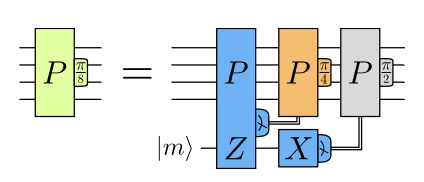
\includegraphics[width=0.5\linewidth]{Figures/magic_T.png}
    \caption{The circuit generate the $\pi/8$ Pauli rotation gate with single $\ket{m}$ states~\cite{Litinski2019gameofsurfacecodes}. It transforms the $\text{CNOT}$ gates into measurements of Pauli operators to satisfied the requirement of lattice surgery, as illustrated in the subsection~\ref{subsec:lattice_surgery}. The equivalence between these two protocols are proved in the Appendix.}
    \label{fig:magic_T}
\end{figure}
\subsection{Fault-tolerant encoded operation}

\begin{theorem}[Legal operations]
    Consider stabilizers built on a $n$-qubits space, the normalizer group of $\mathcal{S}$ over $n$-qubits unitary group $U(n)$, denoted as $N_U(\mathcal{S})$, constitute all operators that map codewords to codewords. If we replace $\mathcal{S}$ by all the $N$-qubits Pauli matrix $G_N$, we defined $N_U(G_N)$. 
\end{theorem}
We first consider the operations in set $N_{U}(G_N) \cap N_U(\mathcal{S}) $. Those operations

\subsection{Fault-tolerant universal computation}

\begin{theorem}[Solovay-Kitaev Algorithm~\cite{dawson2005solovaykitaev}]
    Let $\mathcal{G}$ be an arbitrary subgroup that condensed in group $SU(2)$. Consider an accuracy $\varepsilon$ and a given one-qubit gate $U$, S-K algorithm could find a sequence $S = \prod_{i = 1}^l s_i, s_i \in \mathcal{G}$ such that $\lambda_{max}[(U - S)(U - S)^\dagger] \leq \varepsilon$. The length of the sequence and searching time of this algorithm both satisfied: $l = \mathcal{O}(\ln^{c_l}(1/\varepsilon)), t = \mathcal{O}(\ln^{c_t}(1/\varepsilon))$.
\end{theorem}

\subsection{Lattice surgery\label{subsec:lattice_surgery}}
\paragraph*{Merge operation---\!\!\!}
At the outset, the logical qubits encoded in two surface codes are in states $\ket{\phi_1} = \alpha_1 \ket{0} + \beta_1 \ket{1}$ and $\ket{\phi_2} = \alpha_2 \ket{0} + \beta_2 \ket{1}$ respectively. Between the two surface codes, there are several qubits in the $\ket{0}$ state, corresponding to eigenvalue $+1$ under the $Z$ operator. Prior to any measurement, the quantum state comprises stabilizer states from the subset $S = S_1 \cap S_2 \cap {Z_i}$.

Subsequently, treating the two sets of surface codes and the intermediary qubits as a single surface code, measurements are performed on the $X$ operator along the boundary (depicted as red lines). These measurements transition the stabilizer subset from one stabilizer state to another. The rules governing this transformation are as follows:
 
\begin{theorem}
    Under Pauli measurements $P_m = \frac{\mathbb{I} + (-)^m M}{2}$ with measurement outcomes $m = \pm 1$, the stabilizer subgroup divides into two parts: $S_a$ and $S_c$, where the former anticommutes with $P$ and the latter commutes. Appropriate transformations of generator elements can reduce the elements in $S_a$ to one, denoted as ${A} \cup S_c'$. The state after measurement will be stabilized by the new stabilizer ${(-1)^m M} \cup S_c'$.
\end{theorem}
Using this theorem and the process depicted in the figure, we can observe the evolution of stabilizer subgroup. Note that, depending on the measurement outcome of $-1$, the logical space may be stabilized by Pauli operators of the form $-X_1X_2 X_3 X_4$. Additionally, if the logical states are further specified as $\ket{0}$ and $\ket{1}$, the quantum states not only stabilize the surface code logical states but also the eigenvalues of the $Z$ logical operator (depicted by the deep blue lines). During the measurement process, the product of these logical operators will be preserved. Hence, we deduce the mapping rule for the aforementioned operations as follows: $P_m \ket{r_1}_1 \otimes \ket{r_2}_2 = c_{r_1,r_2,m} \ket{r_1 \oplus r_2}_3$, where $r_1 \oplus r_2 = (r_1 + r_2) ~\text{mod}~2$, and $\ket{\cdot}_3$ refers to the logical qubits after merging in the surface code. To fully determine the mapping rule, we need to specify the coefficients $c_{r_1,r_2,m}$. Before doing so, we need to clarify the logical operators and logical states of the merged logical qubits, as shown in the figure below:
\begin{figure}
    \centering
    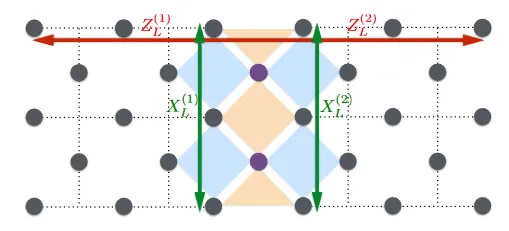
\includegraphics[width=0.5\linewidth]{Figures/merge.png}
    \caption{Enter Caption}
    \label{fig:merge}
\end{figure}
The red lines represent the logical $Z$ operator, while $X^{(2)}$ denotes the logical $X$ operator. It is noteworthy that one could also select $X^{(1)}$ as the logical $X$ operator, but only when the product of measurement outcomes $m = +1$, the state after measurement is the $+1$ eigenstate of $X^{(1)} X^{(2)}$. Both choices are entirely equivalent.

Furthermore, by further fixing the phase of logical states, let $c_{00,m} = 1$ and $c_{01,m} = 1$. Subsequently, based on the following identity:


\begin{align*}
c_{10,m}\ket{0}_3 &= X^{(2)}c_{10,m}\ket{1}_3 \\
&= X^{(2)} P_m \ket{1} \otimes \ket{0} \\
&= X^{(1)}X^{(2)}P_m \ket{0} \otimes \ket{0} \\
&= (-1)^m P_m \ket{0} \otimes \ket{0} \\
&= (-1)^m \ket{0}_3 \\
\end{align*}

We can deduce that $c_{11,m} = c_{10,m} = (-1)^m$. Hence, the merging mapping can be summarized as follows:

\begin{align*}
&P_m \ket{0}_1\otimes \ket{0}_2 = \ket{0}_3, \quad P_m \ket{0}_1\otimes \ket{1}_2 = \ket{1}_3, \\
&P_m \ket{1}_1\otimes \ket{0}_2 = (-1)^m \ket{1}_3, \quad P_m \ket{1}_1\otimes \ket{1}_2 = (-1)^m\ket{0}_3
\end{align*}


\paragraph*{Split operation---\!\!\!}
\begin{figure}
    \centering
    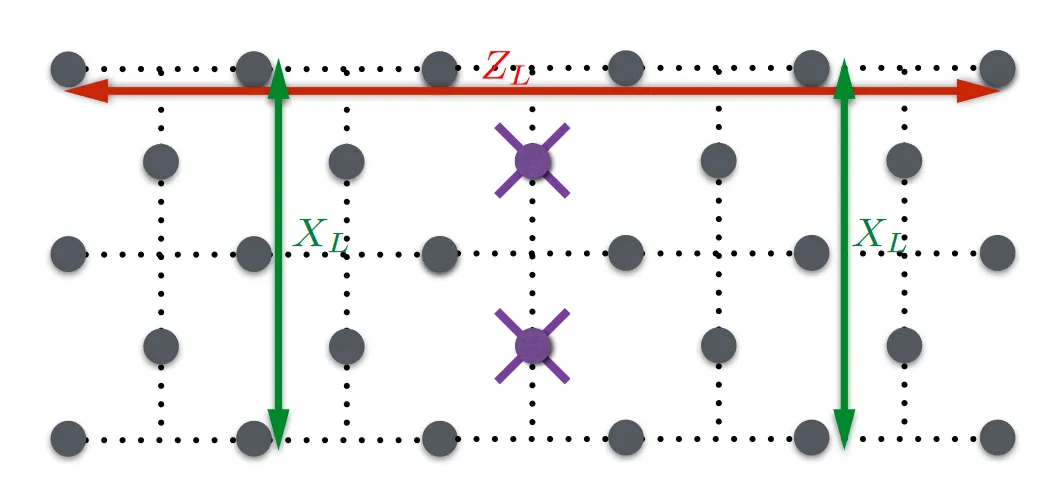
\includegraphics[width=0.5\linewidth]{Figures/split.png}
    \caption{Enter Caption}
    \label{fig:split}
\end{figure}
The split operation, as depicted in the figure, involves measuring the $Z$ operator at the junction point (purple dot). Using a similar method, we can prove the following:

If $m = +1$, $\alpha\ket{+}_3 + \beta\ket{-}_3 \to \alpha\ket{+}_1\ket{+}_2 + \beta\ket{-}_1\ket{-}_2$.

If $m = -1$, $\alpha\ket{+}_3 + \beta\ket{-}_3 \to \alpha\ket{-}_1\ket{+}_2 + \beta\ket{+}_1\ket{-}_2$.

Here, the logical $X$ operator remains consistent with the initial input logical qubits, both chosen as positive products along the boundary line.

Starting from two logical operators in state $\ket{0}_1, \ket{0}_2$, undergoing rough Merge and rough Split operations, their transformation is as follows:

\begin{equation}
\ket{0}_1 \otimes \ket{0}_2 \xrightarrow{merge} \ket{0}_3 = \sqrt{\frac{1}{2}}(\ket{+}_3 + \ket{-}_3) \xrightarrow{split} \left\{  
             \begin{aligned}
             \frac{1}{\sqrt{2}}(\ket{+}_1\ket{+}_2 + \ket{-}_1\ket{-}_2) , m = +1\\   
              \frac{1}{\sqrt{2}}(\ket{-}_1\ket{+}_2 + \ket{+}_1\ket{-}_2) , m = -1  
             \end{aligned}  
\right. 
\end{equation}
\begin{equation}
\ket{0}_1 \otimes \ket{1}_2 \xrightarrow{merge} \ket{1}_3 = \sqrt{\frac{1}{2}}(\ket{+}_3 - \ket{-}_3) \xrightarrow{split} \left\{  
             \begin{aligned}
             \frac{1}{\sqrt{2}}(\ket{+}_1\ket{+}_2 - \ket{-}_1\ket{-}_2) , m = +1\\   
              \frac{1}{\sqrt{2}}(\ket{-}_1\ket{+}_2 - \ket{+}_1\ket{-}_2) , m = -1  
             \end{aligned} 
\right. 
\end{equation}
\begin{equation}
\ket{1}_1 \otimes \ket{0}_2 \xrightarrow{merge} (-1)^m\ket{1}_3 = (-1)^m\sqrt{\frac{1}{2}}(\ket{+}_3 - \ket{-}_3) \xrightarrow{split} \left\{  
             \begin{aligned}  
             \frac{1}{\sqrt{2}}(\ket{+}_1\ket{+}_2 - \ket{-}_1\ket{-}_2) , m = +1\\   
              \frac{1}{\sqrt{2}}(\ket{+}_1\ket{-}_2 - \ket{-}_1\ket{+}_2) , m = -1  
             \end{aligned}  
\right. 
\end{equation}
\begin{equation}
\ket{1}_1 \otimes \ket{1}_2 \xrightarrow{merge} (-1)^m\ket{0}_3 = (-1)^m\sqrt{\frac{1}{2}}(\ket{+}_3 + \ket{-}_3) \xrightarrow{split} \left\{  
             \begin{aligned} 
             \frac{1}{\sqrt{2}}(\ket{+}_1\ket{+}_2 + \ket{-}_1\ket{-}_2) , m = +1\\   
              -\frac{1}{\sqrt{2}}(\ket{-}_1\ket{+}_2 + \ket{+}_1\ket{-}_2) , m = -1  
             \end{aligned} 
\right.  
\end{equation}


It can be observed that the final result is equivalent to performing a projection measurement on two logical qubits in the $X_1X_2$ basis, with the measurement result reflected in the intermediate parameter $m$. Note that, depending on the intermediate processes, many parts of the stabilizer along the boundary may undergo sign changes, $A \to (-1)A$. Similarly, the same process occurs at the smooth edge (where two ZZs are adjacent), allowing fault-tolerant projection measurements in the $Z_1Z_2$ basis to be implemented.
In general, we prove the theorem below:
\begin{theorem}
 Two patches $p_1$ and $p_2$ with a pair of adjacent edges $l_1$ and $l_2$, where specific operators $O_1$ and $O_2$ on these edges correspond to logical operators $L_1$ and $L_2$, respectively. After the merge and split operations on these two pairs of edges, resulting in new patches $p_1'$ and $p_2'$, the logical states under the definition of the same logical operators: $L_1:O_1$; $L_2:O_2$, are equivalent to the results obtained by non-destructively measuring $L_1 \times L_2$ on the original logical states, with the measurement outcome determined by the product $m$ of the merge process measurement results.
\end{theorem}
%%%%%%%%%%%%%%%%%



\bibliography{reference}
\bibliographystyle{ieeetr}
%%%%%%%%%%%%%%%%%%%%%
%%%%%%%%%%%%%%%%%%%%%%%%%
\appendix

\section{Codes simulates quantum gates \label{app:gate_codes}}
\subsection{Gate Fidelity\label{app:gate_fidelity}}

\section{Atom Decay\label{app:atom_decay}}
The Hamiltonian with dual energy levels $\ket{g},\ket{e}$ and single-mode light field (frequency $\omega$) coupled is:
\begin{align}
\mathcal{V} &= \mathbb{P} e \vec{r} \cdot\vec{E} \mathbb{P} \\
&= e  (\langle e|\vec{r}|g\rangle\sigma_- + \langle g|\vec{r}|e\rangle\sigma_+) \cdot [\sqrt{\frac{\hbar \omega }{2\varepsilon_0}}(\vec{f}(\vec{r}) a + \vec{f}^*(\vec{r}) a^\dagger)].
\end{align}
Using chiral symmetry, it is proved that $\langle g|\vec{r}|g\rangle = \langle e|\vec{r}|e\rangle = 0$. Under the interaction representation, the rotation wave approximation can be obtained:
\begin{align}
    \mathcal{V}(t) = \hbar  [g(r) a^\dagger \sigma_{-} e^{-i\delta t} + g^*(r)a \sigma_{+}e^{i\delta t} ],\quad  \delta = \Delta E/\hbar-\omega,
\end{align}
where $g(r) = e\sqrt{\frac{\hbar \omega}{2\varepsilon_0}} \vec{f}(\vec{r}) \cdot \langle g|\vec{r}|e\rangle$. For multi-mode light fields, similarly, the coupling Hamiltonian becomes:
\begin{align}
    \mathcal{V}(t) = \sum_{k,\zeta} \hbar  [g_{k,\zeta}(\vec{r})a_{k,\zeta}^\dagger \sigma_{-} e^{-i\delta_{k} t} + g^*_{k,\zeta}(\vec{r})a_{k,\zeta} \sigma_{+}e^{i\delta_{k} t} ],\quad  \delta_{k} = \Delta E/\hbar-\omega_{k},
\end{align}
where $g_{k,\zeta}(\vec{r}) = e\sqrt{\frac{\hbar \omega_k}{2\varepsilon_0}} \vec{f}_{k,\zeta}(\vec{r}) \cdot \langle g|\vec{r}|e\rangle$. Assuming that the thermal reservoir is large enough and the coupling with atoms is weak enough, the equation for the evolution of the atomic density matrix can be obtained~\cite{Quantumoptics}:
\begin{align}\label{eq:weak-int-reservoir-evol}
\dot\rho_{a}(t) = -\frac{i}{\hbar}Tr_{R} [\mathcal{V}(t), \rho_a(t_i)\otimes\rho_R(t_i)] -\int_{t_i}^t dt' \frac{1}{\hbar^2}Tr_{R} [\mathcal{V}(t), [\mathcal{V}(t'), \rho_a(t)\otimes\rho_R(t_i)]]
\end{align}
For the first parts, we see
\begin{align} 
-\frac{i}{\hbar} Tr_{R}[\mathcal{V}(t), \rho_a(t_i)\otimes\rho_R(t_i)] &=-i \sum_{k,\zeta}  Tr_{R}[g_{k,\zeta}(\vec{r})a_{k,\zeta}^\dagger \sigma_{-} e^{-i\delta_{k} t} + c.c. , \rho_a(t_i)\otimes\rho_R(t_i)] \\
&=-i \sum_{k,\zeta}  Tr_{R}[g_{k,\zeta}(\vec{r})a_{k,\zeta}^\dagger \sigma_{-} e^{-i\delta_{k} t}  , \rho_a(t_i)\otimes\rho_R(t_i)]+c.c. \\
&=-i \sum_{k,\zeta} g_{k,\zeta}(\vec{r})\langle a_{k,\zeta}^\dagger \rangle  e^{-i\delta_{k} t} [\sigma_{-} , \rho_a(t_i)]+c.c. 
\end{align}
For the second integral, we simplified it as:
\begin{align}
 &\frac{1}{\hbar^2}Tr_{R} [\mathcal{V}(t), [\mathcal{V}(t'),\rho_a(t)\otimes\rho_R(t_i)]] \\
&= \frac{1}{\hbar} \sum_{\substack{k',\zeta'}}Tr_{R} [ \mathcal{V}(t), [g_{k',\zeta'}(\vec{r})a_{k',\zeta'}^\dagger \sigma_{-} e^{-i\delta_{k'} t'} +c.c.\ , \rho_a(t)\otimes\rho_R(t_i)]]\\
&= \frac{1}{\hbar}\sum_{\substack{k',\zeta'}}g_{k',\zeta'} (\vec{r})e^{-i\delta_{k'} t'}Tr_{R} [ \mathcal{V}(t), [a_{k',\zeta'}^\dagger \sigma_{-} , \rho_a(t)\otimes\rho_R(t_i)] ] + c.c.\\
&=\sum_{\substack{k',\zeta'\\k.\zeta}}g_{k',\zeta'} (\vec{r})e^{-i\delta_{k'} t'}Tr_{R} [g_{k,\zeta}(\vec{r})a_{k,\zeta}^\dagger \sigma_{-} e^{-i\delta_{k} t} + g^*_{k,\zeta}(\vec{r})a_{k,\zeta} \sigma_{+}e^{i\delta_{k} t} , [a_{k',\zeta'}^\dagger \sigma_{-} , \rho_a(t)\otimes\rho_R(t_i)] ] + c.c.\\
&=\sum_{\substack{k',\zeta'\\k.\zeta}}g_{k',\zeta'} (\vec{r})e^{-i\delta_{k'} t'}g_{k,\zeta}(\vec{r})e^{-i\delta_{k} t}Tr_{R} [a_{k,\zeta}^\dagger \sigma_{-}  , [a_{k',\zeta'}^\dagger \sigma_{-} , \rho_a(t)\otimes\rho_R(t_i)] ] \\
&\quad\quad\quad+ g_{k',\zeta'} (\vec{r})e^{-i\delta_{k'} t'}g^*_{k,\zeta}(\vec{r})e^{i\delta_{k} t}Tr_{R} [a_{k,\zeta} \sigma_{+} , [a_{k',\zeta'}^\dagger \sigma_{-} , \rho_a(t)\otimes\rho_R(t_i)] ] + c.c.\\
&=\sum_{\substack{k',\zeta'\\k.\zeta}} -g_{k',\zeta'} (\vec{r})g_{k,\zeta}(\vec{r})e^{-i\delta_{k'} t'-i\delta_{k} t} \langle a_{k,\zeta}^\dagger a_{k',\zeta'}^\dagger \rangle  \times 2\sigma_{-}\rho_a(t) \sigma_{-} \\
&\quad\quad\quad+ g_{k',\zeta'} (\vec{r})g^*_{k,\zeta}(\vec{r})e^{i\delta_{k} t-i\delta_{k'} t'} \langle a_{k,\zeta} a_{k',\zeta'}^\dagger \rangle [\sigma_{+}\sigma_{-}\rho_a(t) - \sigma_{-}\rho_a(t)\sigma_{+}  ]\\
 &\quad\quad\quad+ g_{k',\zeta'} (\vec{r})g^*_{k,\zeta}(\vec{r})e^{i\delta_{k} t-i\delta_{k'} t'} \langle a_{k',\zeta'}^\dagger a_{k,\zeta}  \rangle  [\rho_a(t)\sigma_{-}\sigma_{+} - \sigma_{+}\rho_a(t)\sigma_{-}]+ c.c.
\end{align}
The photons reservoir coupled to atoms is a canonical ensemble with temperature $T$, and its density matrix is:
\begin{align}
\rho_R = \frac{1}{Z} e^{-\beta H} = \frac{1}{Z} e^{-\beta \sum_{k,\zeta}\hbar \omega_k a_{k,\zeta}^\dagger a_{k,\zeta}} 
\end{align}
Using the condition that the trace of the density matrix is 1, $Z$ can be obtained as follows:
\begin{align}
Z = Tr\ e^{\sum_{k,\zeta}-\beta \hbar \omega_k a_{k,\zeta}^\dagger a_{k,\zeta}} &= \sum_{array~n_{k,\zeta} }\langle n_{k,\zeta} |e^{\sum_{k,\zeta}-\beta \hbar \omega_k a_{k,\zeta}^\dagger a_{k,\zeta}} | n_{k,\zeta} \rangle = \sum_{array~n_{k,\zeta} } \prod_{k,\zeta}e^{-\beta \hbar \omega_k n_{k,\zeta}} \\
&=\prod_{k,\zeta}\sum_{n_{k,\zeta}=0 }^{\infty}e^{\sum_{k,\zeta} -\beta \hbar \omega_k n_{k,\zeta}} = \prod_{k,\zeta} \frac{1}{1 -e^{-\beta \hbar \omega_k }  }
\end{align} 
We could also calculates non-vanish average as below:
\begin{align}
Tr[\rho_R a_{k_1,\zeta_1}^\dagger a_{k_2,\zeta_2}] &= Z^{-1}\sum_{array~n_{k,\zeta} }\langle n_{k,\zeta} |e^{\sum_{k,\zeta}-\beta \hbar \omega_k a_{k,\zeta}^\dagger a_{k,\zeta}} a_{k_1,\zeta_1}^\dagger a_{k_2,\zeta_2}| n_{k,\zeta} \rangle \\
&=Z^{-1}  \delta_{k_1k_2,\zeta_1\zeta_2}\sum_{array~n_{k,\zeta} } e^{\sum_{k,\zeta}-\beta \hbar \omega_k n_{k,\zeta}} n_{k_2,\zeta_2} \\
&=\delta_{k_1k_2,\zeta_1\zeta_2} \frac{1}{e^{\beta\hbar\omega_{k_2}} - 1} := \delta_{k_1k_2,\zeta_1\zeta_2} \bar{n}_{k_2,\zeta_2}.
\end{align}
\begin{align}
Tr[\rho_R  a_{k_2,\zeta_2}a_{k_1,\zeta_1}^\dagger] &= Tr[\rho_R  a_{k_1,\zeta_1}^\dagger a_{k_2,\zeta_2}] + Tr\{\rho_R  [a_{k_2,\zeta_2}, a_{k_1,\zeta_1}^\dagger] \} \\
&=\delta_{k_1k_2,\zeta_1\zeta_2}( \bar{n}_{k_2,\zeta_2}+1).
\end{align}
Plug into Eq.~\eqref{eq:weak-int-reservoir-evol}, we see that:
\begin{align}
\dot\rho_{a} &= -\int_{t_i}^t dt'\{\sum_{\substack{k,\zeta}}  g_{k,\zeta} (\vec{r})g^*_{k,\zeta}(\vec{r})e^{i\delta_{k} (t- t')} ( \bar{n}_{k,\zeta}+1) [\sigma_{+}\sigma_{-}\rho_a(t) -\sigma_{-}\rho_a(t)\sigma_{+} ]\\
 &\quad\quad\quad+ g_{k,\zeta} (\vec{r})g^*_{k,\zeta}(\vec{r})e^{i\delta_{k} (t- t')} \bar{n}_{k,\zeta}[\rho_a(t)\sigma_{-}\sigma_{+} -  \sigma_{+}\rho_a(t)\sigma_{-} ]\}+ c.c.
\end{align}
By introducing the definition of $g_{k,\zeta}$, the equation can be further simplified:
\begin{align}
\sum_{\substack{k,\zeta}}  g_{k,\zeta} (\vec{r})g^*_{k,\zeta}(\vec{r}) &= \sum_{\substack{k,\zeta}}e^2 \frac{\hbar \omega_k}{2\varepsilon_0} |f_{k,\zeta}(\vec{r})|^2 \cdot \varepsilon^i_{k,\zeta}\varepsilon^{j*}_{k,\zeta}\cdot \langle g|r^i|e\rangle  \langle e|r^j|g\rangle 
\end{align}
For light field in free space, $f_{k,\zeta}(\vec{r}) = \frac{1}{\sqrt{V}}e^{i\vec{k}\cdot\vec{r }}$, Moreover, $\sum_{\zeta}\varepsilon^i_{k,\zeta}\varepsilon^{j*}_{k,\zeta} = \delta^{ij} - \hat k^i \hat k ^j$. Then:
\begin{align}
\sum_{\substack{k,\zeta}}  g_{k,\zeta} (\vec{r})g^*_{k,\zeta}(\vec{r}) &= \sum_{k}e^2 \frac{\hbar \omega_k}{2\varepsilon_0} \frac{1}{V} \cdot (\delta^{ij} - \hat k^i \hat k ^j)\cdot \langle g|r^i|e\rangle  \langle e|r^j|g\rangle \\
&=\frac{V}{(2\pi)^3}\int d^3k ~e^2 \frac{\hbar \omega_k}{2\varepsilon_0} \frac{1}{V} \cdot (\delta^{ij} - \hat k^i \hat k ^j)\cdot \langle g|r^i|e\rangle  \langle e|r^j|g\rangle \\
&=\frac{1}{(2\pi)^3}\int dk d\theta ~ 2\pi k^2 \sin\theta ~e^2 \frac{\hbar \omega_k}{2\varepsilon_0}  \cdot (1 - \cos^2\theta)\cdot |\langle g|\vec{r}|e\rangle|^2 \\
&=\frac{4}{3}\frac{1}{(2\pi)^2} |\langle g|e\vec{r}|e\rangle|^2\frac{\hbar c }{2\varepsilon_0}\int dk  k^3   = \frac{\hbar |\langle g|e\vec{r}|e\rangle|^2}{6 \pi^2 \varepsilon_0 c^3}\int d\omega  \omega^3 
\end{align}
We see that $\lim_{t \to \infty}\int_{t_i}^t dt' e^{i\delta_k (t - t')} \approx \pi \delta(\omega_k - \omega_0) +i\times p.v. (\frac{1}{\omega_0 - \omega}), \omega_0 = \Delta E/\hbar$, neglecting the imaginary term, which is one of the contribution to the \textbf{Lamb shifts} after appropriate renormalization. Then
\begin{align}
\dot\rho_{a} &= -\frac{\hbar |\langle g|e\vec{r}|e\rangle|^2\omega_0^3 }{6 \pi \varepsilon_0 c^3}   ( \bar{n}_{k_0,\zeta}+1) [\sigma_{+}\sigma_{-}\rho_a(t) -\sigma_{-}\rho_a(t)\sigma_{+}  ]\\
 &\quad\quad\quad- \frac{\hbar |\langle g|e\vec{r}|e\rangle|^2\omega_0^3 }{6 \pi \varepsilon_0 c^3}  \bar{n}_{k_0,\zeta}[\sigma_{-}\sigma_{+}\rho_a(t) - \sigma_{+}\rho_a(t)\sigma_{-} ]+ c.c. \\
&=-(\Gamma/2)   ( \bar{n}_{k_0,\zeta}+1) [\sigma_{+}\sigma_{-}\rho_a(t) -  \sigma_{-}\rho_a(t)\sigma_{+} ]- (\Gamma/2)  \bar{n}_{k_0,\zeta}[\rho_a(t)\sigma_{-}\sigma_{+} -\sigma_{+}\rho_a(t)\sigma_{-} ]+ c.c.,
\end{align}
where $\Gamma = \frac{\hbar |\langle g|e\vec{r}|e\rangle|^2\omega_0^3 }{3 \pi \varepsilon_0 c^3} $. 

\section{Error propagation pattern in surface code \label{app:error_propagation}}
\begin{figure}[!htbp]
    \centering
    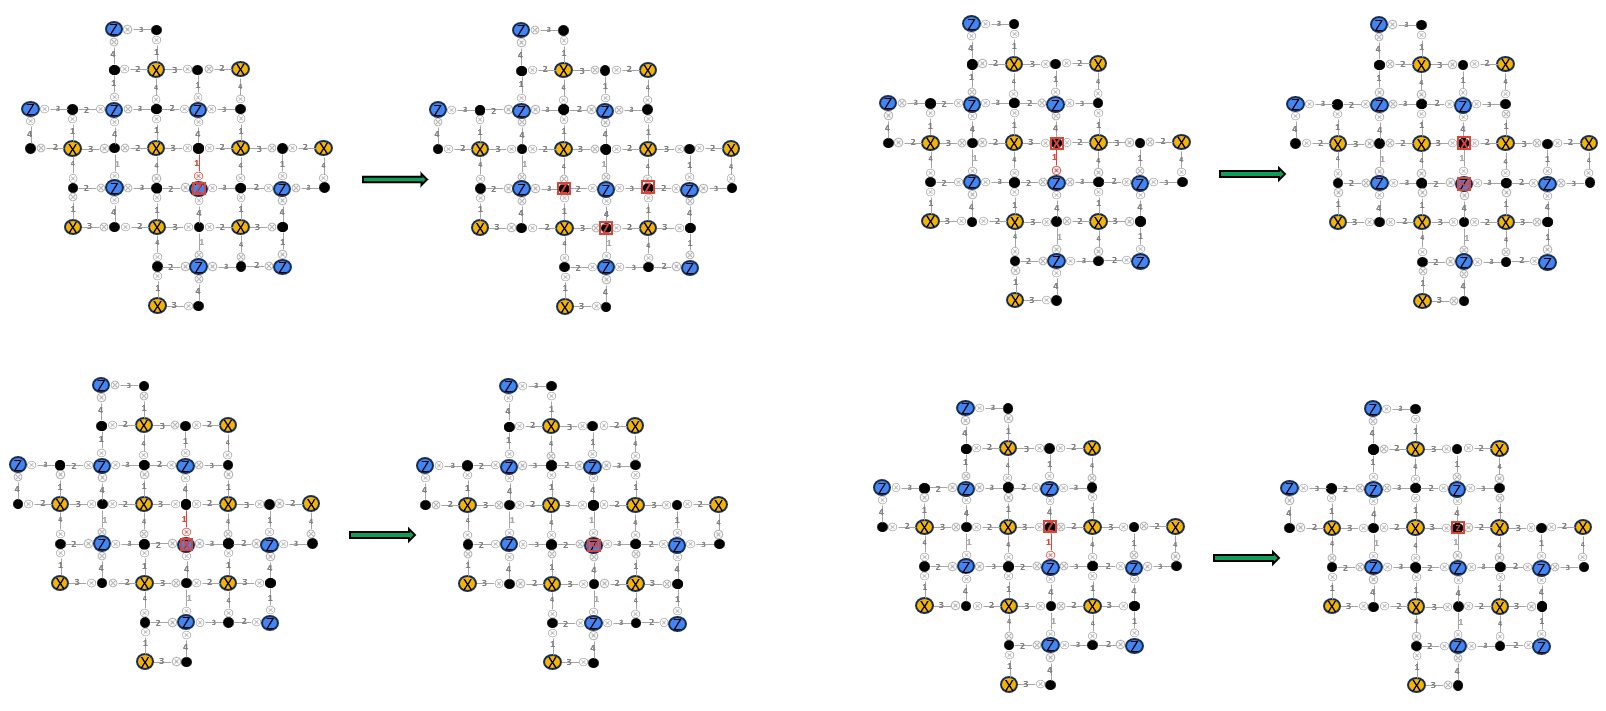
\includegraphics[width=1\linewidth]{Figures/propagate_pattern1.png}
    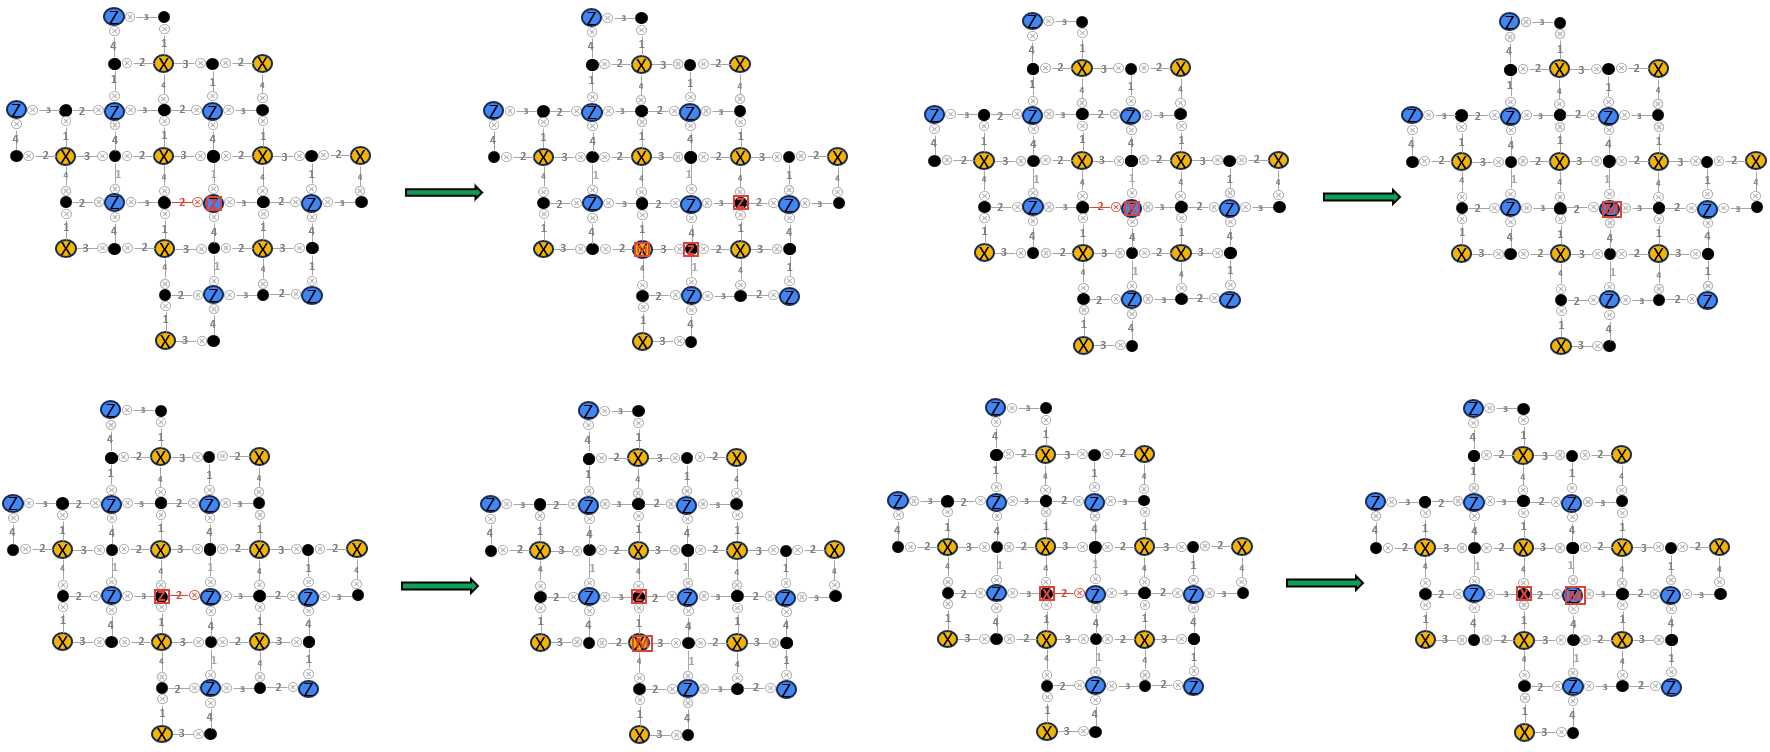
\includegraphics[width=1\linewidth]{Figures/propagate_pattern2.png}
    \label{fig:error_propa_1}
\end{figure}
\begin{figure}[!htbp]
    \centering
    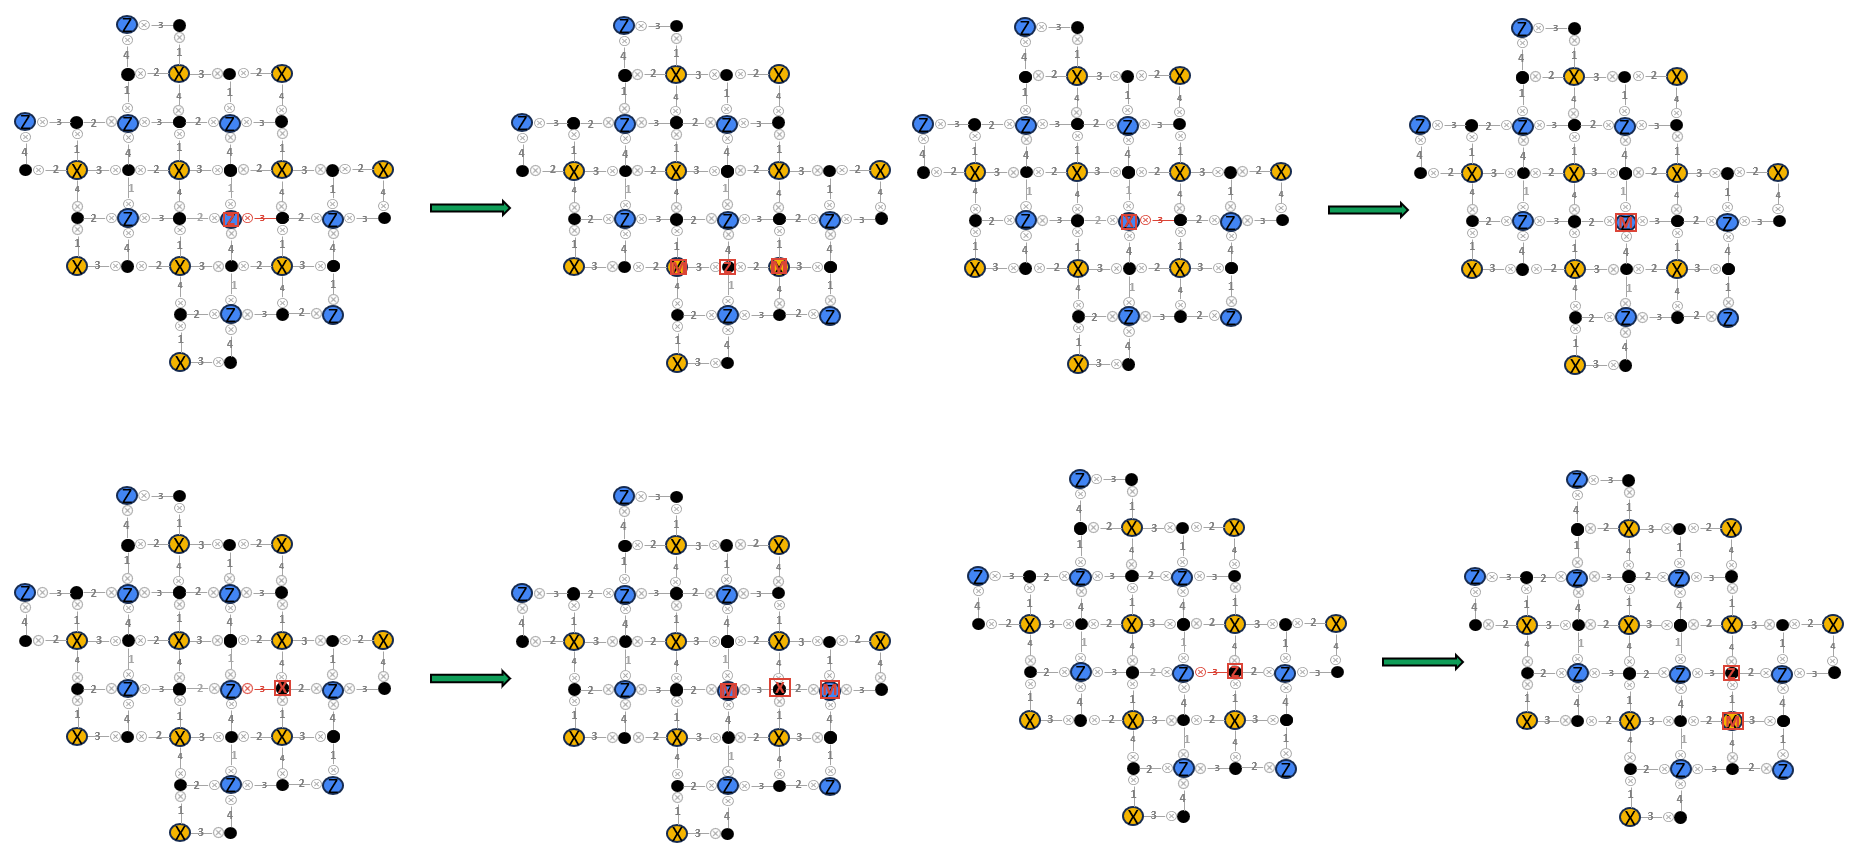
\includegraphics[width=1\linewidth]{Figures/propagate_pattern3.png}
    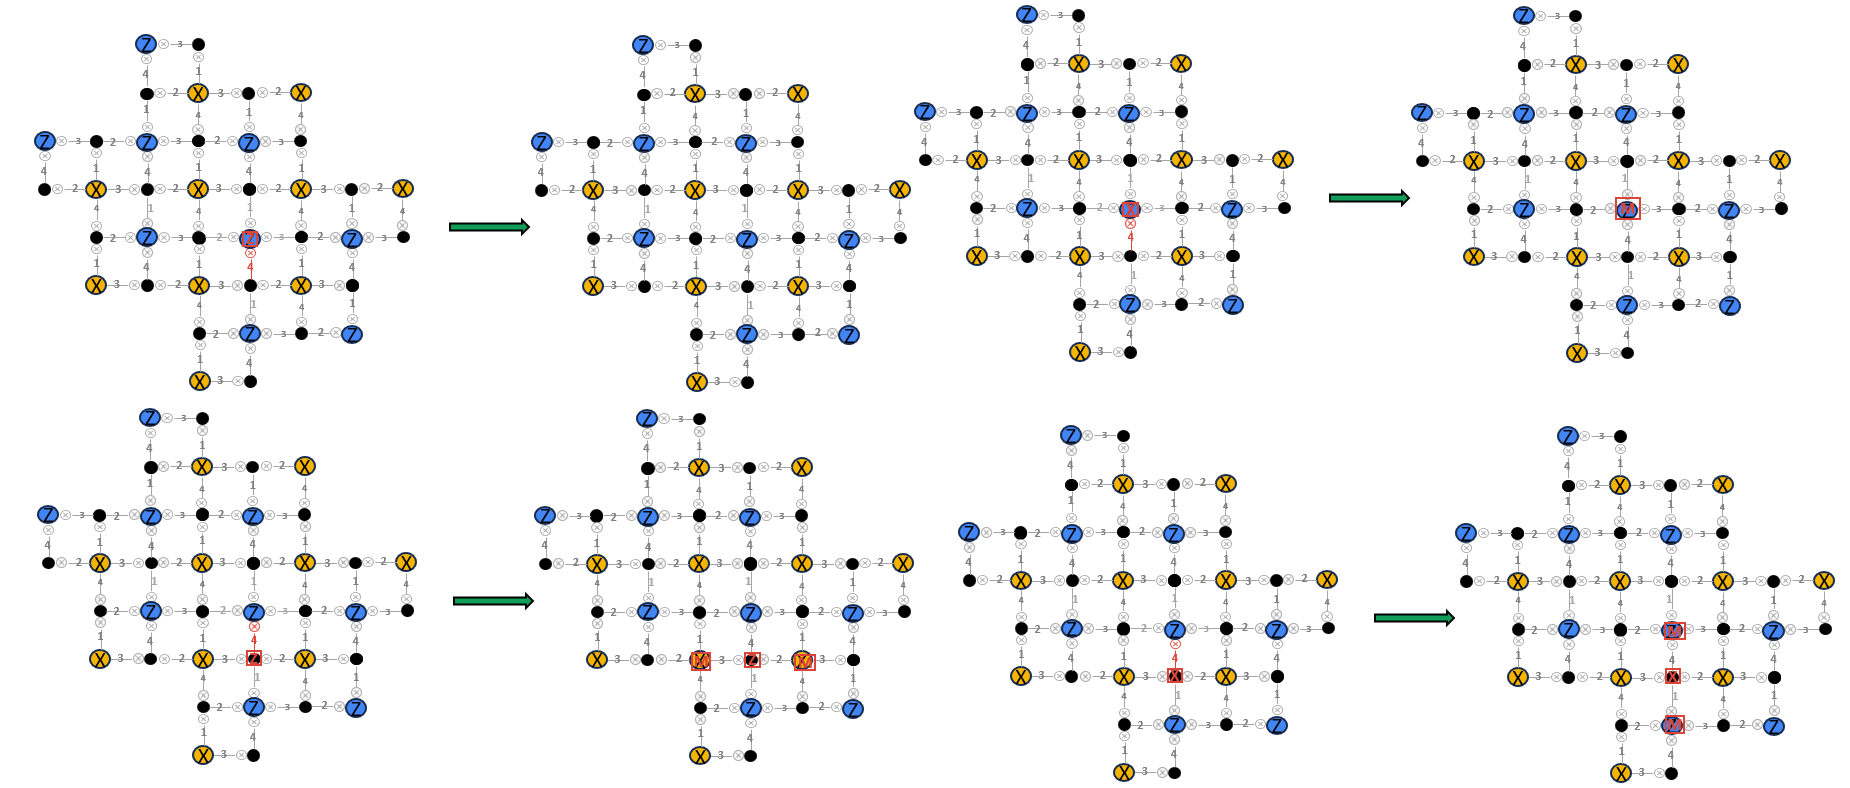
\includegraphics[width=1\linewidth]{Figures/propagate_pattern4.png}
    \label{fig:error_propa_2}
\end{figure}

\newpage
\section{Equivalence of magic state injection}
To show the quivalence between the one-bit teleportation circuit and the measurement $T$ state injection crcuit
in Figure~\ref{fig:magic_T}, we first prove the equation below:
\begin{align}
    e^{i\frac{\pi}{8}\text{Z}_1}\text{CNOT}_{12} = \text{CNOT}_{12} e^{i\frac{\pi}{8}\text{Z}_1 \otimes \text{Z}_2}
\end{align}

\begin{figure}[!htbp]
    \centering
    \begin{quantikz}[row sep=0.3cm, column sep=0.3cm]
        \lstick{$\ket{m}$}    & \qw  & \ctrl{1}  & \gate{SX} \wire[d][1]{c} & \rstick{$T\ket{\psi}$} \\
        \lstick{$\ket{\psi}$} & \qw  & \targ{}      & \meter{} 
      \end{quantikz}
      \hspace{0.1\textwidth}
      \begin{quantikz}[row sep=0.3cm, column sep=0.3cm]
        \lstick{$\ket{m}$}    & \qw  & \ctrl{1}  & \gate{SX} \wire[d][1]{c} &\qw      & \targ{} & \ctrl{1}& \targ{} & \rstick{$\ket{0}$} \\
        \lstick{$\ket{\psi}$} & \qw  & \targ{}   & \meter{}  \wire[r][1]{c} &\gate{X} & \ctrl{-1}& \targ{} & \ctrl{-1} &\rstick{$T\ket{\psi}$}
      \end{quantikz}
\end{figure}

\begin{figure}[!htbp]
    \centering
    \begin{quantikz}[row sep=0.3cm, column sep=0.3cm]
        \lstick{$\ket{m}$}    & \metercw[2]{r_1} & \ctrl{1}  & \gate{SX} \wire[d][1]{c} & \rstick{$T\ket{\psi}$} \\
        \lstick{$\ket{\psi}$} & \qw  & \targ{}      & \meter{} 
      \end{quantikz}
      \hspace{0.1\textwidth}
      \begin{quantikz}[row sep=0.3cm, column sep=0.3cm]
        \lstick{$\ket{m}$}    & \metercw[2]{r_1} & \ctrl{1}  & \gate{SX} \wire[d][1]{c} &\qw      & \targ{} & \ctrl{1}& \targ{} & \rstick{$\ket{0}$} \\
        \lstick{$\ket{\psi}$} & \qw  & \targ{}   & \meter{}  \wire[r][1]{c} &\gate{X} & \ctrl{-1}& \targ{} & \ctrl{-1} &\rstick{$T\ket{\psi}$}
      \end{quantikz}
\end{figure}
\end{document}